\documentclass[12]{article}

\usepackage{gensymb}

\usepackage{float}
\usepackage{float}
\usepackage{booktabs}
\usepackage{multirow}
\usepackage{subcaption}

\usepackage{amsmath}

\usepackage[utf8]{inputenc}
\usepackage[T1]{fontenc}
\setlength{\oddsidemargin}{0.25 in}
\setlength{\evensidemargin}{-0.25 in}
\setlength{\topmargin}{-0.6 in}
\setlength{\textwidth}{6.5 in}
\setlength{\textheight}{8.5 in}
\setlength{\headsep}{0.75 in}
\setlength{\parindent}{0 in}
\setlength{\parskip}{0.1 in}
\usepackage[a4paper,margin=3 cm,footskip=.5cm]{geometry}
\usepackage{textcomp}
\usepackage[table,xcdraw]{xcolor}
\usepackage{hyperref}

\hypersetup{
    colorlinks,
    citecolor=black,
    filecolor=black,
    linkcolor=blue,
    urlcolor=blue
}
\usepackage{graphicx}
\usepackage[inkscapeformat=pdf,inkscapelatex=false]{svg}
%https://www.overleaf.com/project/5ecb94c99100ce000119a4ac
\graphicspath{ {./figs/} }

\begin{document}

\begin{titlepage}
\newcommand{\HRule}{\rule{\linewidth}{0.5mm}}
\setlength{\topmargin}{0 in}
\begin{center}

\begin{figure}[!h]
\centering

\includegraphics [width=0.3\textwidth]{eelogo.png}
\end{figure}

\vspace{10mm}
\Huge{MIDDLE EAST TECHNICAL UNIVERSITY}\\
\vspace{5mm}
{\LARGE ELECTRICAL \& ELECTRONICS ENGINEERING}\\
\vspace{4mm}
\LARGE{Şönt A.Ş.}\\

\HRule\\[0.4cm]
\textsc{\Large{EE464 - STATIC POWER CONVERSION II}}\\
\textsc{\Large{Hardware Project - Flyback Converter\\}}
\textsc{\Large{Simulation Report\\}}
\HRule\\[0.4cm]

\vspace{3mm}

\end{center}
\begin{minipage}{1\textwidth}
		\begin{flushleft}
			\large
			Orhun  \textsc{Taşoğlu - 2094506}\\
			Fahri \textsc{Türedi - 2167435}\\
			Nurettin \textsc{Çavuş - 2094878}
			
		\end{flushleft}
	\end{minipage}

\vspace{10mm}
\begin{center}
\large{23.03.2020}
\end{center}
\end{titlepage}
\tableofcontents
\newpage
\section{Introduction}

One of the most commonly used circuits to perform DC-DC conversion in power electronics applications are Switching Mode Power Supplies (SMPS). To provide a safer output and to comply with international standards of isolation of the output side from the input side is required, especially in grid-connected applications. There are two main topologies of the dc-dc converters with galvanic isolation, which are the Flyback Converters and the Forward Converters. These topologies provide galvanic isolation between their input and output thanks to the isolation transformer placed among the two sides. The isolation transformer provides electrical isolation between the input and output sides of the converter. The isolation transformer also provides larger bandwidth or operation range on the voltage transfer capabilities of the converter by adjusting the primary to secondary turns ratio. Hence, these topologies reduce the weight of the duty ratio on the voltage transfer capability by having the turn ratio of the transformer to make the most of the work. The Flyback Converter topology requires less number of components compared to the Forward Converter. Hence, it has the advantage of reduced cost and size, and higher power density. 

In the previous report, we have presented our topology selection, and the reasoning behind selecting that topology together with the simulation results of the selected topology. We have stated our topology selection as FLY\#1.

Due to the Covid-19 pandemic situation, we, Şönt A.Ş., unfortunately did not have the possibility to complete and implement this project on hardware level. Therefore, in this Final Report, we will provide our project results based on computed aided design and simulations.

In this report, fundamental points of our design, parameter calculations, simulation results with the calculated parameters, component selections, closed loop control system design and key components for building the Flyback Converter topology are explained. First of all, the design methodology of the Flyback Converter is given with the design goals and parameter calculations. The verification of the transformer parameters is also presented in the first part. The magnetic design of the converter transformer is explained in detail in the following section of the report. The transformer core selection and the cable selection for the transformer windings are presented in this section. Next, the simulation results of the constructed Flyback Converter topology depending on the design selections and computed design parameters are given in the Simulation Results section of the report for different source voltage values. Following the simulation results, the component selections for the analog controllers, the semiconductor devices and filter elements in the Flyback Converter topology are presented according to the calculated design parameters and the obtained simulation results. The commercial product selections for the converter switch, diode and output filter capacitor according to the maximum voltage and current stresses over them are given in this section of the report. In the next section of the report, the Efficiency Analysis of the constructed Flyback Converter is presented. The efficiency is analytically calculated for different operating points with different source voltage values, and then compared to the corresponding efficiency values obtained from the simulations of the converter circuit in Simulink for the same operating points. Then, the Thermal Analysis for the converter circuit components is given. The heat sink selections for the MOSFET switch and the diode of the Flyback Converter are shown in this section according to the conducted thermal analysis. In the following section of the report, the closed loop controller design steps for the Flyback Converter circuit are presented. First of all, the derivations for obtaining the AC equivalent circuit model of the Flyback Converter are expressed. The AC equivalent circuit model of the Flyback Converter is presented in the first subsection. Then, the transfer function derivation steps using the obtained AC equivalent circuit model are shown in the following subsection. Following the derivations of the transfer function of the converter topology, the compensator design operation by using the derived transfer function and by considering the possible converter circuit component non-idealities is shown. Finally, the designed closed loop compensated Flyback Converter is simulated and tested under different load change and step input change conditions. The obtained simulation results are presented in the final subsection of this section of the report. In the next section of the report, the steps of the PCB design for the constructed closed loop Flyback Converter circuit are presented. The PCB design details, tips and guidelines are expressed, and the obtained 2D and 3D schematics are shown with the constructed PCB layout of the converter circuit. Finally, the report is concluded by giving the acknowledgements and the final concluding remarks of the project.


\section{Flyback Converter Design}

\begin{figure}[H]
\begin{center}
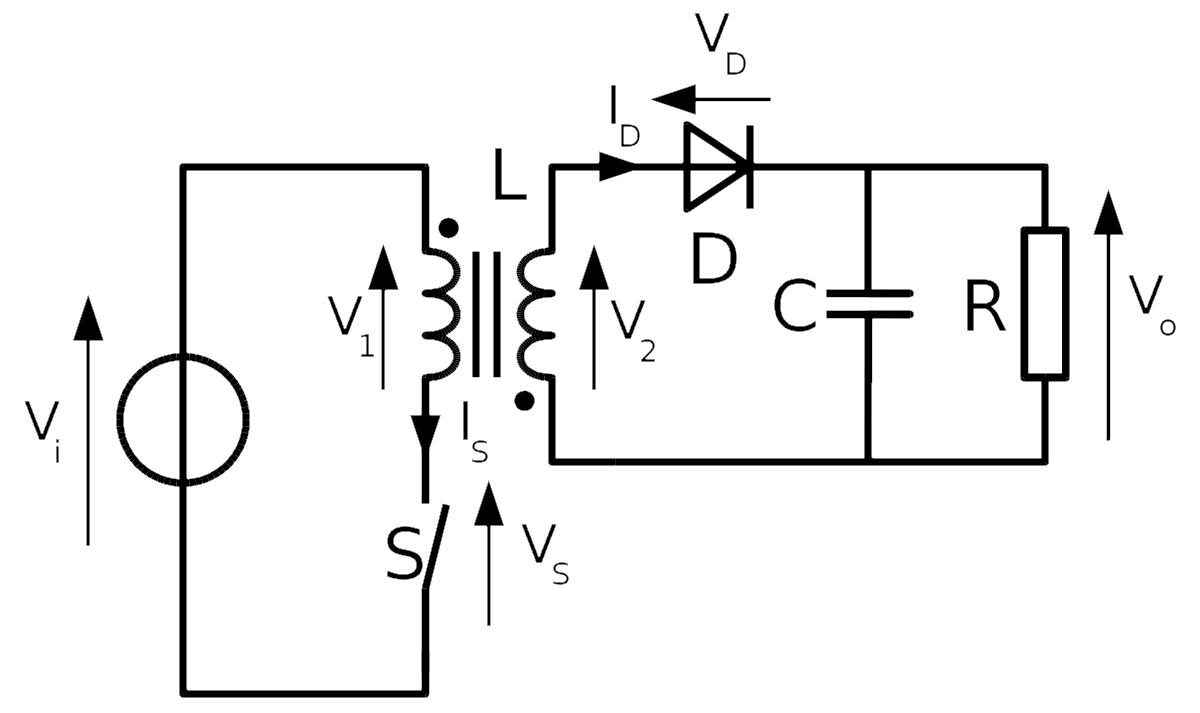
\includegraphics[width=0.6\textwidth]{figures/flybacktop.png}
\caption{Ideal Flyback Converter}
\label{fig:flybacktop}
\end{center}
\end{figure}

The general circuit schematic of an ideal flyback converter topology is given in Figure \ref{fig:flybacktop}. It is a galvanically isolated DC-DC converter with a special feature. That special feature is using the magnetizing inductance of the transformer as an energy storage device, instead of a separate circuit component, which helps reduce the cost, volume and mass of the converter. For our hardware project, we will build a Flyback Converter with extra features to establish the flexibility and performance required to achieve the main requirements and collect bonus points from the Hardware Project. 
\par Our circuit's main controller is UCC28740 by Texas Instruments. It can achieve both current mode and voltage mode control by taking feedback from input and output sides of the converter. For UCC28740 to perform properly, the rest of the circuit should be set to achieve DCM operation at all times. UCC28740 can achieve valley switching, which means it will try to switch the MOSFET at the lowest possible voltage than the primary voltage to reduce the switching losses, and hence increase the efficiency. Those voltage levels are called valley points which are bottoms of the voltage swing at the primary side of the transformer, as seen in Figure \ref{fig:valleyswitch}. The lower voltage level is seen because of the ringing when primary current reaches zero. This kind of Flyback Converter is called Quasi-Resonant Flyback Converter. The selected UCC28740 controller is able to realize this operation mode for the Flyback Converter so that the switching losses are reduced, and hence the efficiency is increased. This operation will also reduce the cooling requirements of the switching device since its switching losses are reduced, which results in smaller sized cooling equipments like heat sinks.

\begin{figure}[H]
\begin{center}
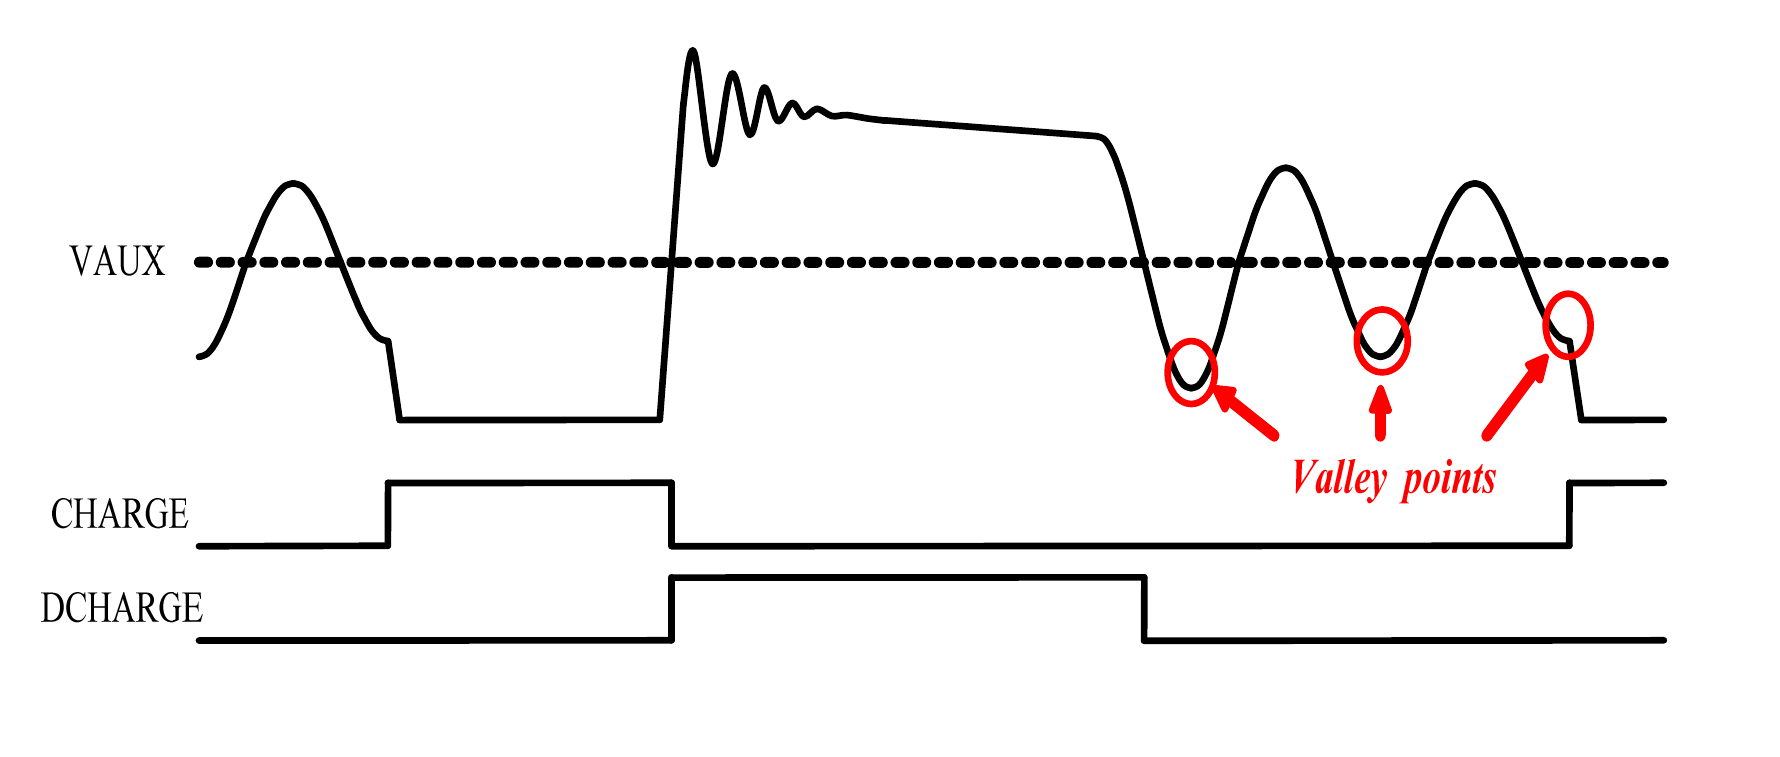
\includegraphics[width=0.6\textwidth]{figures/valleyswitch.png}
\caption{Vallet Points of a Quasi-Resonant Flyback Converter}
\label{fig:valleyswitch}
\end{center}
\end{figure}

The reference design for the mentioned IC is given in Figure \ref{fig:refdesign}.

\begin{figure}[H]
\begin{center}
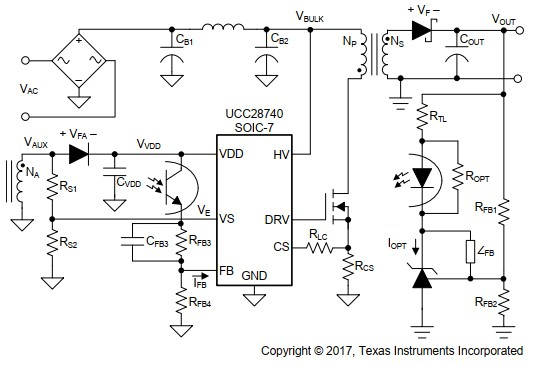
\includegraphics[width=0.8\textwidth]{figures/refdesign.jpg}
\caption{Reference Flyback Converter Design with UCC28740}
\label{fig:refdesign}
\end{center}
\end{figure}

Since our input voltage is directly going to be an adjustable DC voltage, we do not require the bridge rectifier and the rectifier output filter and the EMI filter shown in the above Flyback Converter reference design schematic in Figure \ref{fig:refdesign}.

\subsection{Design Goals}

Complying with the specifications given in the project description, Table \ref{tab:specs} is prepared as a summary. Our design must accomplish the given performance measures. In addition to these, the circuit must employ a closed-loop control. Furthermore, to maximize the functionality and gain bonus points we aimed to go for each positive bonus parts described.

\begin{table}[H]
\centering
\caption{Project Specifications}
\begin{tabular}{|c|c|c|c|c|c|}
\hline
\multicolumn{2}{|c|}{\textbf{Paremeter}}   & \textbf{Min}          & \textbf{Typical}      & \textbf{Max}          & \textbf{Unit}         \\ \hline
\multicolumn{2}{|l|}{\textbf{INPUT}}       & \multicolumn{1}{l|}{} & \multicolumn{1}{l|}{} & \multicolumn{1}{l|}{} & \multicolumn{1}{l|}{} \\ \hline
$V_{in}$  & Input Voltage                       & 24                    & 36                    & 48                    & V (DC)                   \\ \hline
\multicolumn{2}{|l|}{\textbf{OUTPUT}}      &                       &                       &                       &                       \\ \hline
$V_{out}$ & Output Voltage                      & 14.4                  & 15                    & 15.6                  & V (DC)                   \\ \hline
$\Delta V_{out}$ & Output Voltage Ripple & & & 4 & \%
\\ \hline
$I_{out}$ & Output Current                      & -                     & 4                  & -                     & A                     \\ \hline
$P_{out}$ & Output Power                        &                       & 60                    &                       & W                     \\ \hline
     & Line Regulation                     &                       &                       & 2                     & \%                    \\ \hline
     & Load Regulation                     &                       &                       & 2                     & \% 
     \\ \hline
\label{tab:specs}
\end{tabular}
\end{table}

\subsection{Parameter Calculations}

\subsubsection*{Duty Cycle, Turns Ratio, Primary Inductance, Peak Primary Current}

Since the target maximum switching frequency imposed by the limitations of our controllers, it is designated as 45 kHz. $D_{MAGCC}$ is defined as `The secondary diode conduction duty-cycle limit in CC mode, 0.425. which is a device parameter to make sure the transformer is demagnetized and DCM is established. Assuming 500 kHz as the DCM resonance frequency, the times it takes to reach the first valley of $V_{DS}$, $t_R$ should be substracted so that valley switching can be made possible too. To find the maximum duty cycle for constant CCM operation,
\begin{align*}
D_{MAX}&=1-D_{MAGCC}-f_{MAX}\times\frac{t_R}{2}\\
D_{MAX}&=1-0.425-45kHz\times \frac{2 \mu s}{2}=0.53
\end{align*}
\par Since $D_{MAX}$ is known, maximum primary to secondary turns ratio can be determined with the following equation:
\begin{align*}
    N_{PS,MAX}=\frac{D_{MAX} V_{DC,min}}{D_{MAGCC}(V_{O}+v_F})=\frac{0.53\times 24}{0.425*(15.7)}=1.906
\end{align*}

Since the voltage at the current sense feedback pin of the controller, $V_{CST}$ is limited, first we need to determine the $R_{CS}$ to limit the the primary peak current,$I_{PP}$.
\begin{align*}
    R_{CS}&=\frac{V_{CCR}N_{PS}}{2I_{O}}\sqrt{\eta_{transformer}}=74.3m\Omega\\
    I_{PP,MAX}&=\frac{V_{CST,MAX}}{R_{CS}}=\frac{0.773}{0.0746}=10.4A
\end{align*}
Where $V_{CCR}$ is a device parameter called constant-current regulation factor and is equal to 330mV.
To compansate the voltage ripples on the input capactiors, a factor of 0.6 is used. 

%\begin{align*}
%    I_{PPK}=\frac{2P_{out}}{\eta V_{in,min}\sqrt{2}\times 0.8D_{MAX}}=\frac{2\times 60W}{0.85\times %24\sqrt{2}\times 0.6\times 0.53}=13.08A
%\end{align*}


\par To ensure enough energy can be stored in the transformer and DCM operation is established, primary inductance should be specified properly. It should be noted that the transformer will cause losses so they need to taken into consideration too. Assuming 90\% efficiency, magnetizing inductance is calculated.
\begin{align*}
    L_P=\frac{2(V_O+V_F)I_O}{\eta _{transformer}I_{PP,MAX}^2f_{MAX}}=\frac{2\times 15.7\times 4}{0.9\times 10.4^2\times f_{MAX}}=28.67\mu H
\end{align*}
Lastly, since we will need an auxiliary winding to power the controller to sense the primary voltage and utilize low voltage lockout, turns ratio of it should be calculated too. Assuming the lockout voltage to be 15V, and auxiliary diode voltage drop to be 0.5 Volts. Lastly, the upper limit for auxiliary to secondary turns ratio is calculated according to the lowest supply voltage of the controller, $V_{DD,off}$
\begin{align*}
N_{AS,MAX}&=\frac{V_{DD,min}+V_{FA}}{V_O+V_F}=\frac{7.75+0.5}{15+0.7}=0.525\\
N_{PA,MAX}&=\frac{1.9}{0.525}=3.62
\end{align*}

\subsection{Transformer Parameter Verification}
To be able to choose our components properly, the stresses on them should be calculated to make an informed decision. Turns ratio of the transformer affects the peak voltages on the rectifiers. Also, demagnetization and MOSFET on times are should be verified so that the values are in the internal timing limits of our controller.
Reverse voltages on primary and secondary rectifiers are,
\begin{align*}
V_{Reverse,secondary}&=\frac{V_{IN,MAX}\sqrt{2}}{N_{PS}}+V_{O,MAX}=77.8V\\
V_{Reverse,primary}&=\frac{V_{IN,MAX}}{N_{PA}}+V_{VDD}=23.25V
\end{align*}
For MOSFET $V_{DS}$ peak voltage calculation;
\begin{align*}
    V_{DS,peak}=V_{IN,MAX}+(V_O+V_F)N_{PS}=97V
\end{align*}
To find our circuits ON time and Demagnetization times,
\begin{align*}
t_{ON,min}=\frac{L_P}{V_{IN,MAX}}\frac{I_{primary,MAX}}{4}=1.51\mu s\\
t_{Dmag.Min}=\frac{t_{ON,min}V_{IN,MAX}}{N_{PS}(V_O+V_F)}=2.9\mu s
\end{align*}
The minimum required ON time for our controllers is indicated as 280 ns and minimum demagnetizing time is specified as 2.4 $\mu$s. Both criteria are satisfied and our circuit can operate in nominal conditions.
\section{Magnetic Design}

Firstly, the shape of the transformer core is selected as an E-core. Since E-cores can be winded better than toroid cores. To have enough turn numbers on both primary and secondary side, KOOL MU 2510 E CORE(00K2510E090) is selected. Cross-section area of the core is important for turn numbers and core area of the KOOL MU 2510 E CORE is small enough to have 10 turns on the primary side. Parameters of the chosen E-core is given below:

\begin{align}
    A_e &= 35\;mm^2\;(Cross\; Sectional\; Area)\\ l_e &= 48.5\; mm \;(Magnetic\;Path\; Length) \\\mu_c &= 90\; (Relative \;Permeability) \\ B_c &= 1\; T \;(Saturation\; Flux\; Density) \\ Weight &= 5.9\; g\; and\; V_e=1870\; mm^3 \;(Volume) 
\end{align}

According to chosen core secondary turn numbers was calculated.

\begin{align}
    N_S&=\frac{L_P\times I_{peak}}{n\times B_m \times A_e}\\
    N_S&=\frac{28.67\times 10^{-6} \times 10.8 }{1.9 \times 1 \times 35 \times 10^{-6}}=5.2 \;turns
\end{align}

Ratio of the primary turn numbers to secondary turn numbers is calculated, so primary turn number is given below;

\begin{align}
    N_P= n\times N_S = 1.9 \times 5.2 = 10\; turns
\end{align}

In this flyback converter design, UCC28740 analog controller is chosen to control the output voltage and current. To supply V$CC$(7.75V) to UCC28740 analog controller, there is required auxiliary winding come from the transformer. The turn number of the auxiliary winding is calculated below:

\begin{align}
    N_{VCC}= \frac{V_{CC}}{V_O+V_F}\times N_S = \frac{7.75}{12+0.7}\times N_S= 3 \;turns
\end{align}

$$ N_{VCC}= 3\;turns $$

There is a core gap on the E-core. Core gap is crucial because magnetic flux intensity can be controlled by the core gap. If there is smaller gap than required, the core can be saturated and transformer could not work properly. Also the other components of the flyback converter can be damaged due to overload. Required core gap is calculated to have optimum magnetic design. Calculation of the core gap is given below:

\begin{align}
    gap=\frac{\mu_0\times N_P{^2}\times A_e }{L_P}-\frac{I_e}{\mu_c}
    \label{eqn:gap}
\end{align}

$$ gap = \frac{1.256\times 10^{-6}\times 10{^2}\times 35\times 10^{-6}}{28.67\times 10^{-6}}-\frac{48.5\times 10^{-3}}{90}=1.35\times 10^{-3}\;m $$

$$ gap = 1.35\times 10^{-3}\;m = 1.35\;mm $$

To check the calculated values given equations is done. Magnetic flux intensity is crucial, since if it is higher than the saturation level of the core, saturation level of the chosen core is 1 Tesla.

\begin{align}
    B=\frac{\mu_0\times N_P\times I_P}{\frac{I_e}{\mu_c}+gap}&=\frac{1.256\times 10^{-6}\times 10\times 10.8}{\frac{48.5\times 10^{-3}}{90}+3.85\times 10^{-3}}=0.95\\
    V_r&=\frac{N_P}{N_S}\times (V_O+V_F)=24.13 V
\end{align}

0.95 Tesla is lower than saturation level of the core so it is acceptable. Also duty ratio must be lower than 0.53. To check duty ratio of the design, D is calculated below:

\begin{align}
    D=\frac{V_r}{V_r+V{_dc(min)}}=0.5
\end{align}

\subsection{Transformer Selection}

According to the design calculations and simulation results of the ideal Flyback Converter circuit presented in the Simulation Report, the peak current of the transformer is equal to 10.8 Ampere, turn ratio of the transformer is 1.9:1, primary turn number of transformer is determined as 10, and the secondary turn number is equal to 5. Transformer primary side voltage is between 24-48 V which is input voltage range. To obtain the required turn numbers, the cross-section area of the core must be smaller than 40 $mm^2$ and core saturation density of the available cores B = 1 Tesla. According to the required cross-section area range, KOOL MU 2510 E core is chosen. The cross-sectional area of the chosen core is 38.5 $mm^2$. The effective magnetic path length of the core is 48.5 $mm$. The permeability of the core is given as 90$\mu$.

$$ turns\; ratio = 1.9 \approx 2 $$

$$ N_P = 10\; turns $$

$$ N_S = 5\; turns $$

The Figure \ref{fig:Permeability} below shows the detailed dimensions and the permeability and inductance per turn squared values of the KOOL MU 2510 E core.

\begin{figure}[!h]
\centering
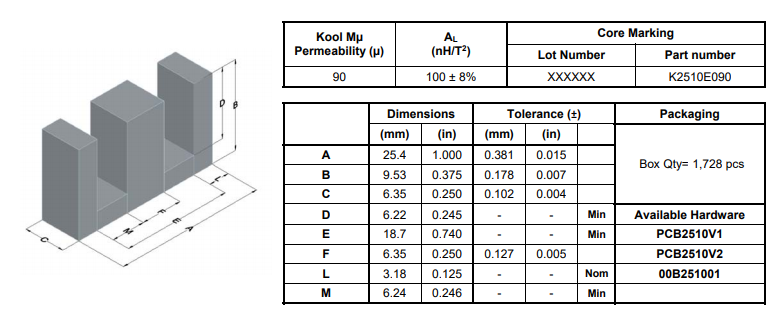
\includegraphics [width=1\textwidth]{figures/core.png}
\caption{Detailed dimensions of the E core and relative permeability of core }
\label{fig:Permeability}
\end{figure}

The cross-sectional area is important to decide turn numbers and the air gap between E cores. Information about cross-sectional area and magnetic path length is given Figure \ref{fig:Csa}. As can be seen from equation \eqref{eqn:gap2}, the gap is directly affected by path length and relative permeability, so both the magnetic path length and the relative permeability are also crucial for the magnetic design.

\begin{align}
    gap=\frac{\mu_0\times N_P^2 \times A_e}{L_P}-\frac{l_e}{\mu_c}
    \label{eqn:gap2}
\end{align}
Magnetic flux density of the core can be calculated by given formula;
\begin{align}
    B=\frac{\mu_0\times N_P\times A_e}{\frac{l_e}{\mu_c}+gap}
    \label{eqn:fluxB}
\end{align}

As seen from equation \eqref{eqn:fluxB}, magnetic flux density depends on the cross-sectional area, magnetic path length and relative permeability of the core. The cross-sectional area and relative permeability are limited since the core can be saturated. Magnetic flux density is inversely proportional with air gap length and magnetic path length. As can be seen from Figure \ref{fig:SFD}, saturation flux density of the KOOL MU magnetic cores is equal to 1 Tesla. The core shape, cross-sectional area and magnetic path length are chosen according to the saturation flux density of the KOOL MU magnetic core, which is 1 Tesla.

$$ B_{sat} = 1\;Tesla $$

\begin{figure}[!h]
\centering
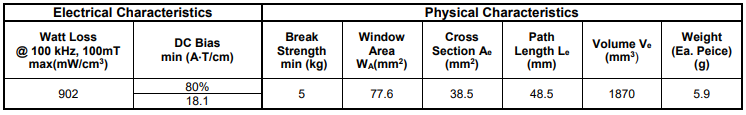
\includegraphics [width=1\textwidth]{figures/area vs.png}
\caption{Cross sectional area and Path Length of core }
\label{fig:Csa}
\end{figure}
\begin{figure}[H]
\centering
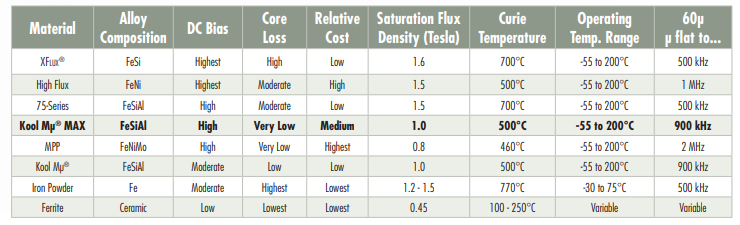
\includegraphics [width=1\textwidth]{figures/permeability.png}
\caption{Saturation Flux Densities of various magnetic cores }
\label{fig:SFD}
\end{figure}

\subsection{Cable Selection}

In order to make the proper cable selection for the designed Flyback Converter circuit, we, first of all, need to determine the skin depth at the selected switching or operating frequency.

$\delta$= Skin Depth\\
$\rho$= Resistivity of Material\\
$\mu_r$= Relative Permeability of Cable\\
$\mu_0$= Permeability Constant = $4\pi\times 10^{-7}$\\
$f_s$ = switching frequency = 45 kHz \\

Then, the skin depth is given by the following formula in equation \eqref{eqn:skin}.

\begin{align}
    \delta=\sqrt{\frac{\rho}{\pi\times f\times \mu_r\times \mu_0}}
    \label{eqn:skin}
\end{align}

For copper cables, the formula in equation \eqref{eqn:skin} can be reduced to the following simplified for as given in equation \eqref{eqn:skin2}, below.

\begin{align}
    \delta=\frac{7.5}{\sqrt{f_s}}\; cm = \frac{75}{\sqrt{f_s}}\; mm
    \label{eqn:skin2}
\end{align}

Then, we can compute the skin depth at the switching frequency of $f_s$ = 45 kHz, as follows:

$$ \delta=\frac{75}{\sqrt{45000}}\; mm $$

$$ \delta= 0.3535\; mm $$

At 45 kHz switching frequency, skin depth of copper cable is equal to 0.3535 mm.

Furthermore, we also need to determine the maximum RMS current that flows through the primary or the secondary winding terminals of the transformer in order to make the cable selection with the proper dimensions and sizes.

Since the voltage ratings of the output side (15 V) of the designed Flyback Converter is less than the input side voltage ratings (24-48 V), the output current ratings of the converter is higher than the input current ratings. In other words, the secondary side current ratings of the transformer is higher than the primary side current ratings. Therefore, for the appropriate cable selection, we need to consider the maximum RMS current rating on the secondary (output) side of the transformer.

The average output current of the Flyback Converter can be determined from the following power relation.

\begin{align}
    P_{out} = V_{out}I_{out}
    \label{eqn:power}
\end{align}

If we substitute the average output power of 60 W and the average output voltage of 15 V into the above equation \eqref{eqn:power}, we can obtain the average output current as 4 A, as follows:

$$ I_{out} = \frac{P_{out}}{V_{out}} = \frac{60}{15} = 4\;A $$

$$ I_{out} = 4\;A $$

The maximum ripple in the secondary side current of the transformer is equal to the maximum current ripple on the output diode of the Flyback Converter topology. The maximum current ripple in the diode current is measured as 19.42 A in the simulations with the ideal Flyback Converter circuit in Simulink as also stated in the Simulation Report.

$$ \Delta i_{D,max} = 19.42\;A $$

After computing the average current and the maximum ripple current values in the transformer secondary side, we can, finally, calculate the maximum RMS current value on the secondary side of transformer by using the following relation given in equation \eqref{eqn:rms_current}.

\begin{align}
    I_{sec,RMS} = \sqrt{I_{out}^2 + (\frac{\Delta i_{D,max}}{2})^2}
    \label{eqn:rms_current}
\end{align}

Hence, if we substitute the computed current values into the equation \eqref{eqn:rms_current}, the maximum RMS current value of the secondary side current of the transformer is obtained as follows:

$$ I_{sec,RMS} = \sqrt{4^2 + (\frac{19.42}{2})^2} = \sqrt{16 + 94.28} = \sqrt{110.28} = 10.5\;A\; (RMS) $$

$$ I_{sec,RMS} = 10.5\;A\; (RMS) $$

Hence, the analytical result for the secondary side RMS current value of the transformer is obtained as 10.5 A (RMS).

In the simulations with the ideal Flyback Converter circuit in Simulink, the maximum RMS current at the secondary side of the transformer is measured as 8.138 A (RMS).

$$ I_{sec,RMS} = 8.138\;A\; (RMS) $$

This current value is close to the above analytically computed RMS current value of 10.5 A. However, since the analytical equation that is utilized to compute the secondary RMS current value is not exactly correct, and does not give exact results, we will use the RMS current value obtained from the simulations of the ideal Flyback Converter circuit in Simulink in order to make the cable selection for the transformer.

Hence, the secondary side maximum RMS current of the transformer is obtained as 8.138 A (RMS).

The maximum current density that a copper cable can carry is given as J = 4 $A/mm^2$.

Then, the minimum required cable cross-sectional area is found as follows:

\begin{align}
    A_{conductor} = \frac{I_{sec,RMS}}{J}
    \label{eqn:area_cond}
\end{align}

Then, the minimum required conductor area for the selected cable is found as follows by substituting the necessary parameters into the equation \eqref{eqn:area_cond}.

$$ A_{conductor} = \frac{8.138}{4} = 2.0345\;mm^2 $$

$$ A_{conductor} = 2.0345\;mm^2 $$

However, since this required conductor area value is large, and since it will result in a very thick and large cable selection, we decided to use some cables in parallel in order to reduce the current stress over each cable, and hence also help us to select much thinner and small cables. Furthermore, using parallel cables also provides the benefit of reduced copper resistances and hence copper losses. One another advantage of using parallel cables is that they help to achieve the optimal wounding geometry around the transformer window area, which helps to reduce the leakage fluxes, proximity and skin effect disruptions.

As a result, we decided to utilize 4 cables in parallel for the primary and secondary windings of the transformer.

This, in result, reduces the minimum required conductor area for the selected cable to one fourth of the previously computed minimum required conductor area value.

Hence, the new minimum required conductor area with using 4 cables in parallel is obtained as follows:

$$ A_{conductor} = \frac{2.0345}{4} = 0.508625\;mm^2 $$

$$ A_{conductor} = 0.509\;mm^2 $$

As a result, we can select cable AWG\#19 considering the given conductor area limitations.

\textbf{Selected Cable: }AWG\#19
The parameters of the selected cable is given below.

\begin{itemize}
    \item The diameter of the cable: 0.91186 mm
    \item The conductor cross-sectional area of the cable: 0.653 $mm^2$
    \item Ohms per km: 26.40728 \ohm/km
\end{itemize}

After making the cable selection, we can finally compute the fill factor of the designed transformer for the Flyback Converter.

First of all, we need to compute the total conductor area that fills the window area of the designed transformer. In order to compute the total conductor area, we, first of all, need to multiply the cross-sectional area of the selected cable with the number of paralleled cables, which is 4. Then, the total conductor area is obtained by multiplying the above computed value with the total number of turns of the primary and the secondary side of the transformer.

\begin{align}
    \sum A_{conductor} = (N_P + N_S)\times A_{conductor}\times 4
    \label{eqn:total_area}
\end{align}

Then, the total conductor area is obtained as follows by substituting the necessary parameters into the equation \eqref{eqn:total_area} above.

$$ \sum A_{conductor} = (10 + 5)\times 0.653\times 4 = 15\times 0.653\times 4 = 39.18\;mm^2 $$

$$ \sum A_{conductor} = 39.18\;mm^2 $$

Finally, the fill factor can be obtained by using the following relation.

\begin{align}
    fill\;factor = \frac{\sum A_{conductor}}{A_{window}}
    \label{eqn:fill_factor}
\end{align}

The window area of the selected core is equal to 77.62 $mm^2$ as given in its datasheet, as shown in Figure \ref{fig:SFD} above.

As a result, we can compute the fill factor for the designed transformer by substituting the above parameters into equation \eqref{eqn:fill_factor}, as follows.

$$ fill\;factor = \frac{39.18}{77.62} = 0.5 $$

$$ fill\;factor = 0.5\; (50\%) $$

This value is quite reasonable since it shows that our window area utilization is quite good with nearly 50\%. Furthermore, it is also
lower than the practical upper limit of 0.6 (or 60\%) for round copper cables. This value of fill factor shows that we are utilizing nearly the half of the window area of the designed transformer, which is a quite reasonable design.

Next, we nee to compute the DC and AC resistances of the transformer windings.

First of all, we start by computing the DC resistances of the transformer primary and secondary windings.

The mean length per turn value for the selected core is computed as follows by using the core dimensions given in its datasheet as shown in Figure \ref{fig:Permeability} above.

\begin{align}
    MLT = \pi(\frac{E + F}{2})
    \label{eqn:mlt}
\end{align}

Then, the mean length per turn value for the selected core is obtained as follows by substituting the necessary dimension values in equation \eqref{eqn:mlt} from its datasheet.

$$ MLT = \pi \times (\frac{18.7 + 6.35}{2}) = \pi \times 12.525 = 39.348\; mm $$

$$ MLT = 39.348\; mm $$

Next, the total length of the primary winding is obtained by multiplying the MLT value with the primary number of turns $N_P$.

\begin{align}
    Length_{Pri} = MLT\times N_P
\end{align}

Hence, the total length of the primary winding is found as follows:

$$ Length_{Pri} = 39.348\times 10 = 393.48\; mm $$

We can round this value up to 400 mm.

$$ Length_{Pri} \approx 400\; mm $$

Similarly, we can compute the total length of the secondary winding of the transformer by multiplying the MLT value with the secondary number of turns $N_S$.

\begin{align}
    Length_{Sec} = MLT\times N_S
\end{align}

Hence, the total length of the secondary winding is found as follows:

$$ Length_{Sec} = 39.348\times 5 = 196.742\; mm $$

We can round this value up to 200 mm.

$$ Length_{Sec} \approx 200\; mm $$

In order to compute the DC resistances of the primary and the secondary windings, we need to multiply the resistance per mm ratio of the selected cable with calculated primary and secondary winding lengths. Finally, the DC resistance values of the primary and secondary windings are obtained by dividing the result by 4 since we used 4 cables in parallel in the construction of the primary and the secondary windings.

The per km resistance of the selected cable is given as:

$$ R = 26.40728\; \ohm / km  $$

Then, the per mm resistance of the selected cable is obtained as:

$$ R = 26.40728\times 10^{-6}\; \ohm / mm  $$

Finally, the DC resistance of the primary winding is computed as follows:

\begin{align}
    R_{DC,pri} = \frac{R\times Length_{Pri}}{4} 
\end{align}

$$ R_{DC,pri} = \frac{26.40728\times 10^{-6}\times 400}{4} = 2.64\;m\ohm $$

$$ R_{DC,pri} = 2.64\;m\ohm $$

Similarly, the DC resistance of the secondary winding is computed as follows:

\begin{align}
    R_{DC,sec} = \frac{R\times Length_{Sec}}{4} 
\end{align}

$$ R_{DC,sec} = \frac{26.40728\times 10^{-6}\times 200}{4} = 1.32\;m\ohm $$

$$ R_{DC,sec} = 1.32\;m\ohm $$

Now, after computing the DC resistances of the primary and the secondary winding, we need to compute the AC resistances of the primary and the secondary winding.

For that, first of all, we need to compute the effective cross-sectional area of the cables at the operating (switching) frequency of $f_s$ = 45 kHz.

The effective cross-sectional area of the cables is computed as follows by using the computed skin depth value.

\begin{align}
    A_{effective} = \pi\times ((\frac{D}{2})^2 - (\frac{D}{2} - \delta)^2)
\end{align}

$$ A_{effective} = \pi\times ((\frac{0.91186}{2})^2 - (\frac{0.91186}{2} - 0.3535)^2) $$

$$ A_{effective} = \pi\times ((0.45593)^2 - (0.10238)^2) = 0.620\;mm^2 $$

$$ A_{effective} = 0.620\;mm^2 $$

Finally, the AC resistances of the primary and the secondary winding are obtained as follows:

For primary:

\begin{align}
    R_{AC,pri} = R_{DC,pri}\times \frac{A_{conductor}}{A_{effective}}
\end{align}

$$ R_{AC,pri} = 2.64\times \frac{0.653}{0.620} $$

$$ R_{AC,pri} = 2.78\;m\ohm $$

For secondary:

\begin{align}
    R_{AC,sec} = R_{DC,sec}\times \frac{A_{conductor}}{A_{effective}}
\end{align}

$$ R_{AC,sec} = 1.32\times \frac{0.653}{0.620} $$

$$ R_{AC,sec} = 1.39\;m\ohm $$

We can tabulate the computed AC resistance values as shown in the following table.

\begin{table}[H]
    \centering
    \caption{AC Coil Resistances}
    \begin{tabular}{|c|c|}
    \hline
\textbf{Parameter}   & \textbf{Value}             \\ \hline
$R_{AC,pri}$ & 2.78\;m\ohm \\ \hline
$R_{AC,sec}$ & 1.39\;m\ohm \\ \hline
    \end{tabular}
    \label{tab:resistance_ac}
\end{table}
\section{Simulation Results}

In this section, we will provide the simulation results of the non-ideal Flyback Converter circuit for two different source (input) voltage level.

In the simulations, we will use the open loop model of the Flyback Converter circuit. Therefore, the duty cycle of the converter switch will be controlled by hand (using a PWM Generator block in Simulink).

The simulations will be much more detailed compared to the simulations provided in the Simulation Report, where we used the ideal Flyback Converter circuit model with the non-idealities of the circuit components and elements are ignored. However, in this report, we will make our similations including the non-idealities of the converter circuit components and elements. The non-ideal semiconductor characteristics for the MOSFET switch and the diode will be included to the simulations. We will also include the non-idealities of the output capacitor. Furthermore, the non-idealities in the magnetic design such as the coil resistances of the primary and the secondary side windings of the transformer and the leakage inductances of the primary and the secondary side windings of the transformer will be included in the simulations.

The non-idealities of the converter circuit components will be taken from their data sheet, and inserted into the simulation model.

The non-idealities in the magnetic design of the transformer such as coil resistances and the leakage inductance will be taken from the analytical calculations provided in the magnetic design section.

The following Figure \ref{fig:fly_schema} shows the Simulink model of the non-ideal Flyback Converter circuit. 

\begin{figure}[H]
\begin{center}
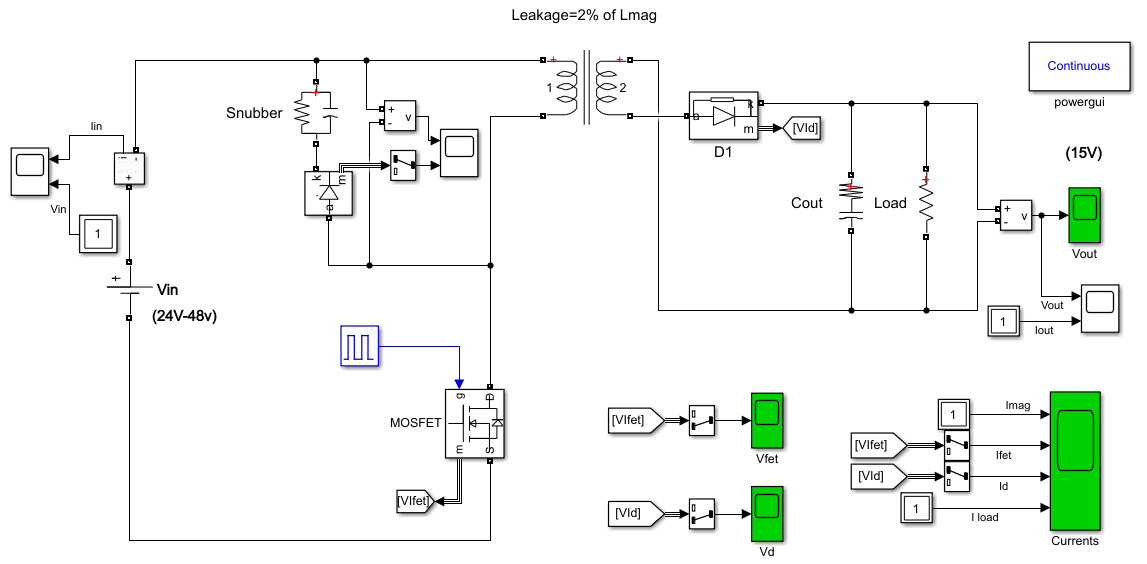
\includegraphics[width=1\textwidth]{figures/flyback_schematic.png}
\caption{Simulink Schematic of the Flyback Converter Circuit}
\label{fig:fly_schema}
\end{center}
\end{figure}

If we investigate this simulation model from its input to output about what is included and what is not included, we will, first of all, notice that we have included an RCD snubber to the primary side of the transformer. This RCD snubber is included in the simulation model due to the transformer leakage inductances. The close view of the used RCD snubber is shown in Figure \ref{fig:fly_snubber}, below.

\begin{figure}[H]
\begin{center}
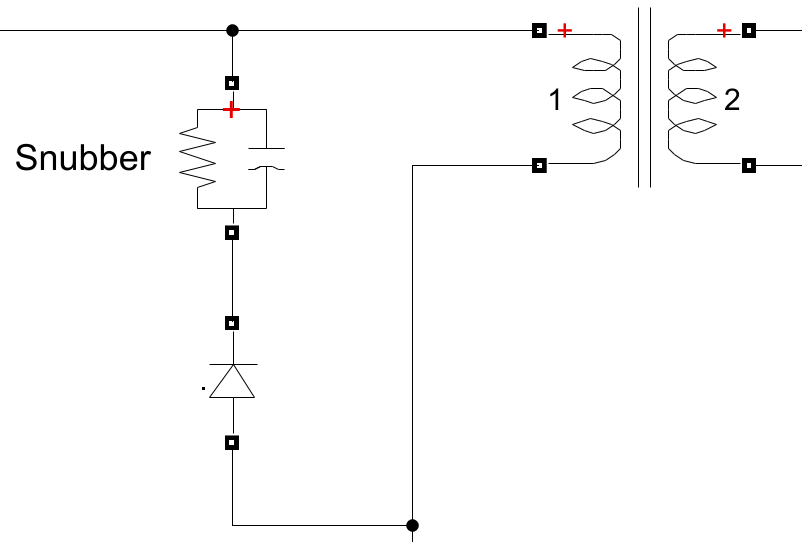
\includegraphics[width=0.4\textwidth]{simulations/snubber.png}
\caption{RCD Snubber Circuit}
\label{fig:fly_snubber}
\end{center}
\end{figure}

The primary side leakage inductance of the transformer increases the voltage stress on the MOSFET switch to infinity, which inevitably causes the MOSFET switch of the Flyback Converter to blow up, and hence resulting in circuit failures.

In order to prevent the voltage spikes that goes to infinity and to reduce the voltage stress over the MOSFET switch of the converter, we included an RCD snubber across the primary terminals of the transformer. The designed RCD snubber circuit provides the leakage inductance current a path to discharge over itself and the parallel RC circuit of the snubber. As a result, we provide a safe path for the leakage inductance current to flow, which reduces the voltage and current stresses over the MOSFET switch of the converter during its off (open) period.

The resistance R and the capacitance C parameters of the designed RCD snubber is as given below.

$$ R_S = 10\;k\ohm $$
$$ C_S = 47\;nF $$

Without the RCD snubber, the MOSFET voltage makes a spike and goes to infinity, which would undoubtedly damage the MOSFET and the break the converter circuit operation.

Next, as mentioned, we have also included the coil resistances and the leakage inductances of the primary and the secondary windings of the designed transformer in the simulation.

The following Figure \ref{fig:trans_para} shows the parameters entered to the linear transformer block in the simulation model.

\begin{figure}[H]
\begin{center}
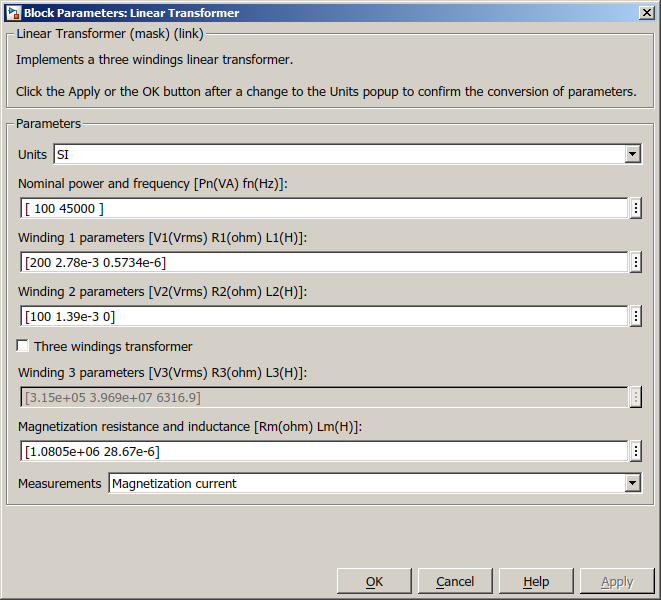
\includegraphics[width=0.4\textwidth]{simulations/transformer_para.png}
\caption{Transformer Block Parameters}
\label{fig:trans_para}
\end{center}
\end{figure}

We have entered the calculated coil resistances of the primary and the secondary windings of the designed transformer as calculated in the magnetic design section.

The entered coil resistance values are as follows:

$$ R_{pri,ac} = 2.78\;m\ohm $$
$$ R_{sec,ac} = 1.39\;m\ohm $$

We also entered the total leakage inductance of the primary and the secondary windings of the transformer as the 2\% of the magnetizing inductance of the transformer.

$$ L_m = 28.67\;\micro H $$

$$ L_{leakage} = 0.02\times L_m $$
$$ L_{leakage} = 0.02\times 28.67 = 0.5734\;\micro H $$

The total leakage inductance of the primary and the secondary windings of the transformer is included in the primary side of the transformer as shown in Figure \ref{fig:trans_para}.

Next, we have also included the non-idealities of the selected output capacitor. We included the ESR value of the selected capacitor to the simulation model.

The ESR value of the output filter capacitor is given as follows.

$$ R_{ESR} = 20\;m\ohm $$

Finally, we have also included the non-idealities of the semiconductor devices: MOSFET and diode. The non-idealities like on resistance and forward voltage drop are taken from their datasheet, and included in the simulation model.

The following figures show the included parameters for the semiconductor devices: MOSFET and diode.

\begin{figure}[H]
\begin{center}
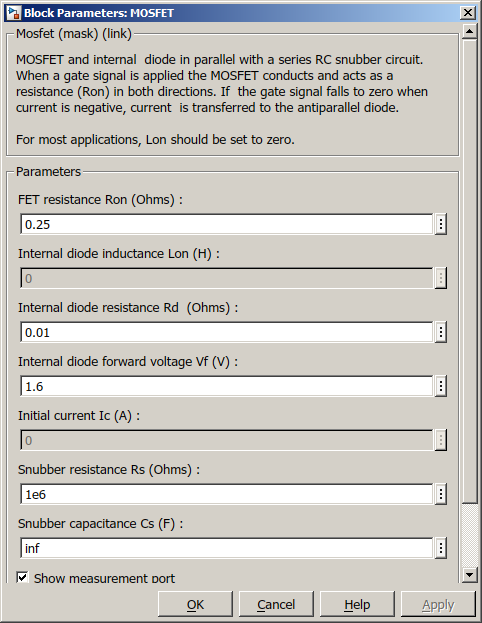
\includegraphics[width=0.4\textwidth]{simulations/mosfet_para.png}
\caption{MOSFET Block Parameters}
\label{fig:mosfet_para}
\end{center}
\end{figure}

\begin{figure}[H]
\begin{center}
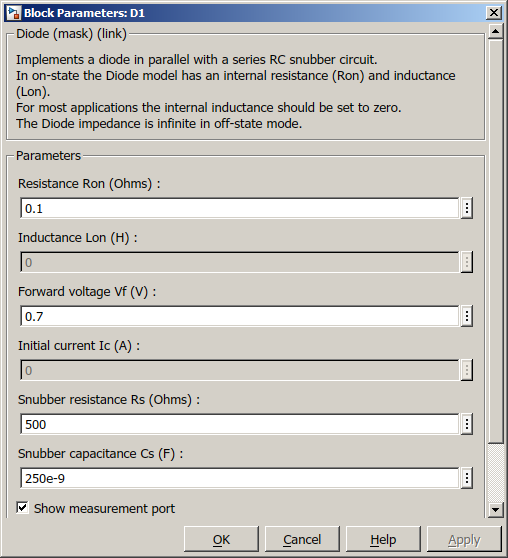
\includegraphics[width=0.4\textwidth]{simulations/diode_para.png}
\caption{Diode Block Parameters}
\label{fig:diode_para}
\end{center}
\end{figure}

Hence, we have completed the explanation of the included non-idealities in the simulation model. 

Now, we will explore the simulation results of the constructed non-ideal Flyback Converter circuit model for different source (input) voltage values.

\subsection{Simulation Results for $V_{in} = 24V$}

In this subsection, the simulation results of the constructed non-ideal Flyback Converter are presented for the source (input) voltage of 24V.

We have obtained the duty cycle value D which makes the average output voltage equal to 15V at steady-state as 60.4\% after a number of trials. This duty cycle value was determined as 52.7\% for the ideal Flyback Converter circuit model in the Simulation Report. However, in this case, it is required to increase this duty cycle value to 60.4\% due to the additional voltage drop effects of the non-idealities in the circuit components.

$$ D = 60.4\% $$

The Figure \ref{fig:tran_out24} shows the transient waveform of the output voltage of the converter for the source voltage of 24V.

\begin{figure}[H]
\begin{center}
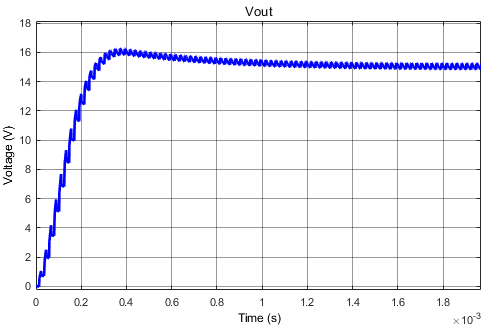
\includegraphics[width=0.7\textwidth]{figures/Vout_transient_24.png}
\caption{Transient Output Voltage Waveform of the Flyback Converter}
\label{fig:tran_out24}
\end{center}
\end{figure}

The steady-state waveform of the output voltage of the converter circuit for the source voltage of 24V is shown in Figure \ref{fig:out24}.

\begin{figure}[H]
\begin{center}
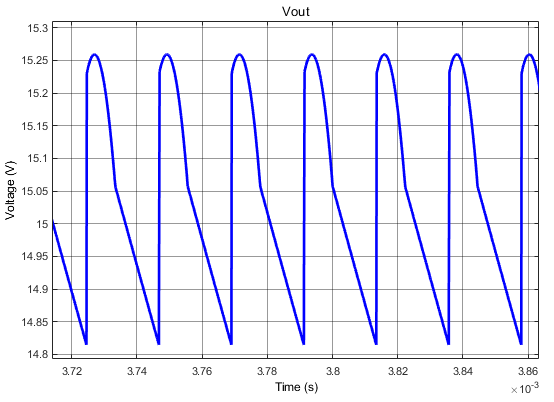
\includegraphics[width=0.7\textwidth]{figures/Vout_24.png}
\caption{Output Voltage Waveform of the Flyback Converter}
\label{fig:out24}
\end{center}
\end{figure}

It is observed that the output voltage oscillates around 15V on average. The peak value of the output voltage is measured as 15.26V, and the minimum value of the output voltage is measured as 14.81V. Hence, the steady-state peak to peak ripple at the output voltage of the converter is computed as 0.45V. This peak to peak ripple value is observed to be less than the maximum of 0.6V peak to peak ripple specified in the project limitations for the output voltage.

$$ \Delta V_{out} = 0.45V < 0.60V $$

The steady-state waveforms of the output voltage and the load current of the converter circuit for the source voltage of 24V are shown on the same plot in Figure \ref{fig:viout_24}.

\begin{figure}[H]
\begin{center}
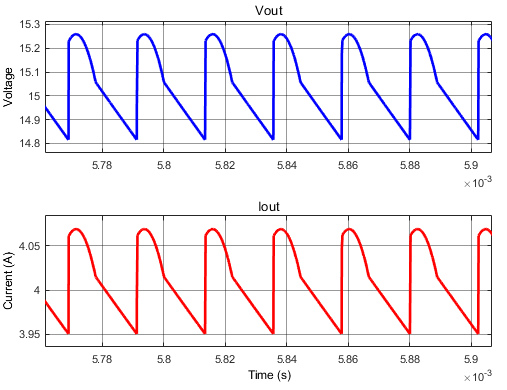
\includegraphics[width=0.7\textwidth]{figures/V_I_out_24.png}
\caption{Output Voltage and Load Current Waveforms of the Flyback Converter}
\label{fig:viout_24}
\end{center}
\end{figure}

It is observed from the load current waveform that it has an average of 4A, and oscillates around 4A. The maximum load current is equal to 4.07A while the minimum load current is equal to 3.95A. As a result, there is a 0.12A peak to peak ripple in the load current.

The steady-state current waveforms of magnetizing inductor, MOSFET switch and diode of the converter circuit for the source voltage of 24V are shown on the same plot in Figure \ref{fig:currents24}.

\begin{figure}[H]
\begin{center}
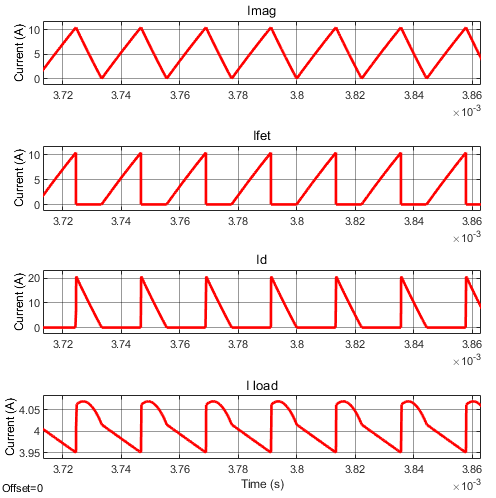
\includegraphics[width=0.7\textwidth]{figures/currents_24.png}
\caption{Current Waveforms of the Flyback Converter}
\label{fig:currents24}
\end{center}
\end{figure}

It is observed that the maximum repetitive current through the MOSFET switch is equal to 10A. In addition, the maximum repetitive current through the diode is approximately equal to 20A.

The peak repetitive current though the diode is the two times that of the MOSFET switch due to the 2:1 turns ratio between the transformer primary and secondary winding ($N_P/N_S = 2$). This makes the current levels at the secondary side of the transformer double of the current levels at the primary side of the transformer.

It is also observed that the magnetizing inductor current changes between 0A and 10A. It is also seen from the magnetizing inductor current that the converter circuit is operating slightly in the DCM mode. The magnetizing inductance current drops to 0A in each switching cycle.

Furthermore, we can state that the frequency of ripples in the output voltage, load current, MOSFET current and diode current is equal to the switching frequency $f_s$, which is equal to 45 kHz. As a result, the presented voltage and current waveforms has a ripple frequency of 45 kHz.

The MOSFET voltage waveform of the Flyback Converter circuit is shown in Figure \ref{fig:mos24}, below.

\begin{figure}[H]
\begin{center}
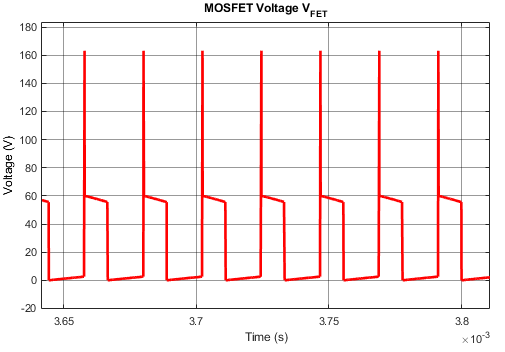
\includegraphics[width=0.7\textwidth]{figures/V_FET_24.png}
\caption{MOSFET Voltage Waveform of the Flyback Converter}
\label{fig:mos24}
\end{center}
\end{figure}

It is observed that maximum voltage stress over the MOSFET during its off (open) period is normally equal to around 60V. However, due to the leakage inductance of the transformer, we observe some voltage spikes in the MOSFET voltage waveform during the turn off operations of the switch. These voltage spikes are present despite the existence of the RCD snubber in the simulation model. However, the magnitude of the voltage spikes are greatly reduced and limited thanks to the existence of the RCD snubber on the primary side of the transformer. Normally, we would expect to see voltage spikes with a magnitude of around infinity on the MOSFET voltage in the absence of the RCD snubber. However, in the presence of the RCD snubber, we observe that the peak amplitude of the voltage spikes in the MOSFET voltage waveform is limited to around 160V as seen from Figure \ref{fig:mos24} above.

The selected commercial MOSFET model STP17NK40ZFP is able to withstand the drain to source voltages as high as 400V. This indicates that the selected switch model is able to withstand the measured voltage spike with a peak of 160V.

The diode voltage waveform of the Flyback Converter circuit is shown in Figure \ref{fig:diode24}, below.

\begin{figure}[H]
\begin{center}
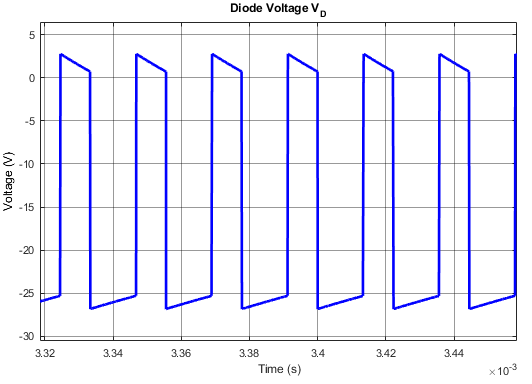
\includegraphics[width=0.7\textwidth]{figures/V_diode_24.png}
\caption{Diode Voltage Waveform of the Flyback Converter}
\label{fig:diode24}
\end{center}
\end{figure}

It is observed that the maximum reverse voltage across the diode is around -25V. The selected commercial diode model has a peak repetitive reverse blocking voltage rating of 100V. This result shows that the selected diode is able to operate properly under these steady-state conditions.

The snubber circuit voltage and current waveforms of the Flyback Converter circuit are shown in Figure \ref{fig:snubber24}, below.

\begin{figure}[H]
\begin{center}
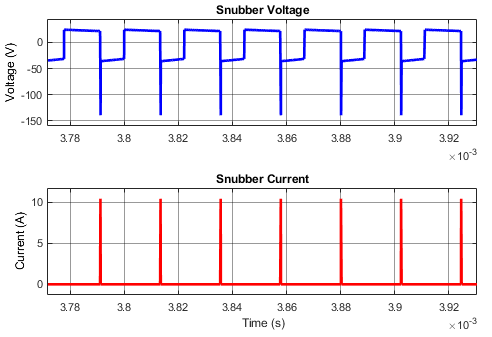
\includegraphics[width=0.7\textwidth]{figures/snubber_24.png}
\caption{RCD Snubber Voltage and Current Waveforms of the Flyback Converter}
\label{fig:snubber24}
\end{center}
\end{figure}

The input current waveform of the Flyback Converter circuit is shown in Figure \ref{fig:Iin24}, below.

\begin{figure}[H]
\begin{center}
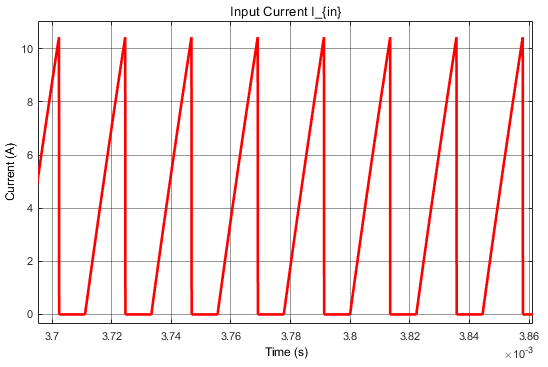
\includegraphics[width=0.7\textwidth]{figures/I_in_24.png}
\caption{Input Current Waveform of the Flyback Converter}
\label{fig:Iin24}
\end{center}
\end{figure}

The input current has a peak of approximately 11A in steady-state operation. The average input current is equal to 3.226A.

The Table \ref{tab:sim24} below shows the average voltage, current and power values obtained from the simulations of the Flyback Converter circuit with $V_{in} = 24V$. 

\begin{table}[H]
    \centering
    \caption{Average Voltage, Current and Power Values Obtained from Simulation}
    \begin{tabular}{|c|c|c|c|c|c|}
    \hline
\textbf{Parameter}   & \textbf{Value}          & \textbf{Parameter}      & \textbf{Value}          & \textbf{Parameter} & \textbf{Value}         \\ \hline
$V_{in}$ & 24V & $I_{in}$ & 3.226A & $P_{in}$ & 77.43W \\ \hline
$V_{out}$ & 15.04V & $I_{out}$ & 4.011A & $P_{out}$ & 60.34W \\ \hline
$I_D$ & 4.012A & $I_{FET}$ & 3.222A & $\eta$ & 78\% \\ \hline
$V_{out(max)}$ & 15.26V & $V_{out(min)}$ & 14.81V & $\Delta V_{out}$ & 0.45V \\ \hline
    \end{tabular}
    \label{tab:sim24}
\end{table}

Then, the efficiency of the Flyback Converter circuit for the input voltage $V_{in} = 24V$ is obtained as follows:

\begin{align}
    Efficiency = \eta = \frac{P_{out}}{P_{in}}
    \label{eqn:eff24}
\end{align}

$$ Efficiency = \eta = \frac{60.34W}{77.43W} = 0.78\;(78\%) $$

Hence, it is seen from the simulations of the non-ideal Flyback Converter circuit in Simulink that it has an efficiency of around 78\% for the source voltage of 24V. This efficiency level is satisfactory considering that all possible non-idealities in the converter circuit components are included in the simulation model except for the core losses of the designed transformer. 

The detailed efficiency analysis of the Flyback Converter circuit including the core losses of the designed transformer is presented in the Efficiency Analysis section of the report.

It is also observed from Table \ref{tab:sim24} that the output voltage ripple $\Delta V_{out}$ is equal to 0.45V, which is less than the project limitations of 0.6V (4\% of the output average voltage). This result shows that the designed Flyback Converter circuit is able to meet the project specifications defined on the output voltage limitations successfully.

$$ \Delta V_{out} = 0.45V < 0.60V $$

\subsection{Simulation Results for $V_{in} = 48V$}

In this subsection, the simulation results of the constructed non-ideal Flyback Converter are presented for the source (input) voltage of 48V.

We have obtained the duty cycle value D which makes the average output voltage equal to 15V at steady-state as 29.4\% after a number of trials. This duty cycle value was determined as 26.25\% for the ideal Flyback Converter circuit model in the Simulation Report. However, in this case, it is required to increase this duty cycle value to 29.4\% due to the additional voltage drop effects of the non-idealities in the circuit components.

$$ D = 29.4\% $$

The Figure \ref{fig:tran_out48} shows the transient waveform of the output voltage of the converter for the source voltage of 48V.

\begin{figure}[H]
\begin{center}
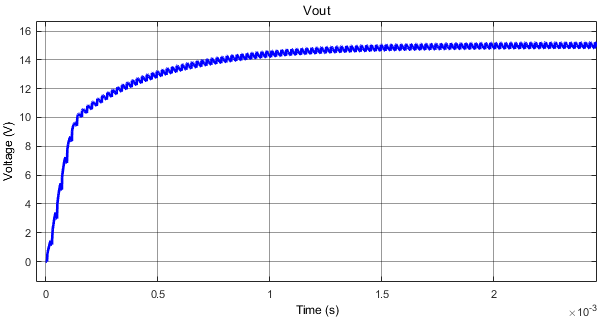
\includegraphics[width=0.7\textwidth]{figures/Vout_transient2_48.png}
\caption{Transient Output Voltage Waveform of the Flyback Converter}
\label{fig:tran_out48}
\end{center}
\end{figure}

The steady-state waveform of the output voltage of the converter circuit for the source voltage of 48V is shown in Figure \ref{fig:out48}.

\begin{figure}[H]
\begin{center}
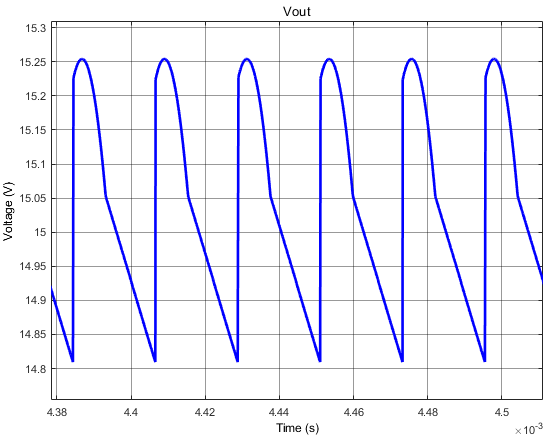
\includegraphics[width=0.7\textwidth]{figures/Vout_48.png}
\caption{Output Voltage Waveform of the Flyback Converter}
\label{fig:out48}
\end{center}
\end{figure}

It is observed that the output voltage oscillates around 15V on average. The peak value of the output voltage is measured as 15.25V, and the minimum value of the output voltage is measured as 14.81V. Hence, the steady-state peak to peak ripple at the output voltage of the converter is calculated as 0.44V. This peak to peak ripple value is observed to be less than the maximum of 0.6V peak to peak ripple specified in the project limitations for the output voltage.

$$ \Delta V_{out} = 0.44V < 0.60V $$

The steady-state waveforms of the output voltage and the load current of the converter circuit for the source voltage of 48V are shown on the same plot in Figure \ref{fig:viout_48}.

\begin{figure}[H]
\begin{center}
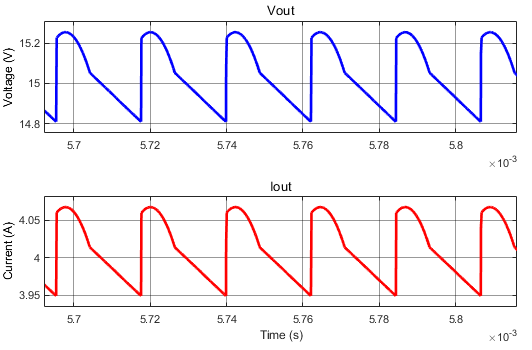
\includegraphics[width=0.7\textwidth]{figures/V_I_out_48.png}
\caption{Output Voltage and Load Current Waveforms of the Flyback Converter}
\label{fig:viout_48}
\end{center}
\end{figure}

It is observed from the load current waveform that it has an average of 4A, and oscillates around 4A. The maximum load current is equal to 4.07A while the minimum load current is equal to 3.95A. As a result, there is a 0.12A peak to peak ripple in the load current.

The steady-state current waveforms of magnetizing inductor, MOSFET switch and diode of the converter circuit for the source voltage of 48V are shown on the same plot in Figure \ref{fig:currents48}.

\begin{figure}[H]
\begin{center}
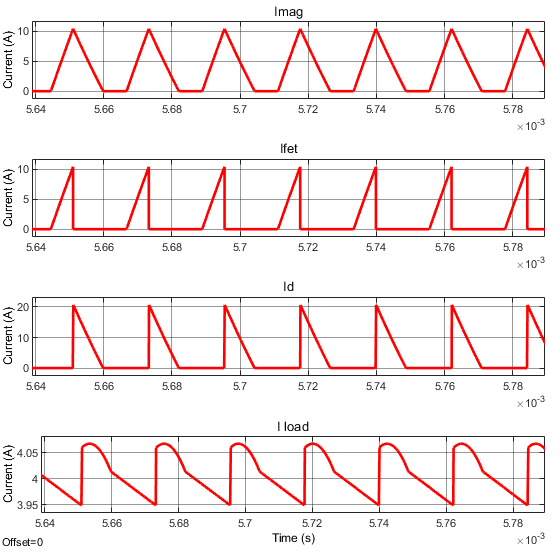
\includegraphics[width=0.7\textwidth]{figures/currents_48.png}
\caption{Current Waveforms of the Flyback Converter}
\label{fig:currents48}
\end{center}
\end{figure}

It is observed that the maximum repetitive current through the MOSFET switch is equal to 10A. In addition, the maximum repetitive current through the diode is approximately equal to 20A.

The peak repetitive current though the diode is the two times that of the MOSFET switch due to the 2:1 turns ratio between the transformer primary and secondary winding ($N_P/N_S = 2$). This makes the current levels at the secondary side of the transformer double of the current levels at the primary side of the transformer.

It is also observed that the magnetizing inductor current changes between 0A and 10A. We can also clearly observe the DCM mode of operation of the converter circuit for the source voltage value of 48V. The magnetizing inductance current drops down to 0A in each switching cycle, and stays at 0A for a short period until the next switching cycle begins.

Furthermore, we can state that the frequency of ripples in the output voltage, load current, MOSFET current and diode current is equal to the switching frequency $f_s$, which is equal to 45 kHz. As a result, the presented voltage and current waveforms has a ripple frequency of 45 kHz.

The MOSFET voltage waveform of the Flyback Converter circuit is shown in Figure \ref{fig:mos48}, below.

\begin{figure}[H]
\begin{center}
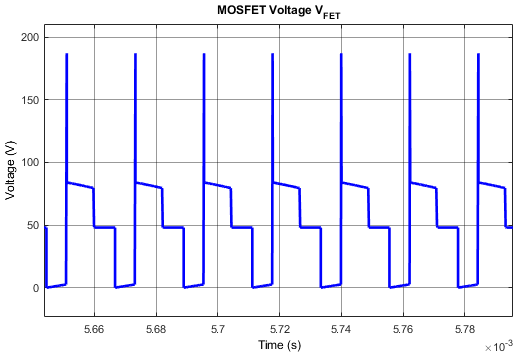
\includegraphics[width=0.7\textwidth]{figures/V_FET_48.png}
\caption{MOSFET Voltage Waveform of the Flyback Converter}
\label{fig:mos48}
\end{center}
\end{figure}

It is observed that maximum voltage stress over the MOSFET during its off (open) period is normally equal to around 80V. However, due to the leakage inductance of the transformer, we observe some voltage spikes in the MOSFET voltage waveform during the turn off operations of the switch. These voltage spikes are present despite the existence of the RCD snubber in the simulation model. However, the magnitude of the voltage spikes are greatly reduced and limited thanks to the existence of the RCD snubber on the primary side of the transformer. Normally, we would expect to see voltage spikes with a magnitude of around infinity on the MOSFET voltage in the absence of the RCD snubber. However, in the presence of the RCD snubber, we observe that the peak amplitude of the voltage spikes in the MOSFET voltage waveform is limited to around 200V as seen from Figure \ref{fig:mos48} above.

The selected commercial MOSFET model STP17NK40ZFP is able to withstand the drain to source voltages as high as 400V. This indicates that the selected switch model is able to withstand the measured voltage spike with a peak of 200V.

We are also able to observe the DCM operation of the converter circuit for the source voltage value of 48V from the MOSFET voltage waveform. It is seen that the MOSFET voltage drops down from approximately 80V to 48V during the off (open) period off the switch. This action occurs at the moment when the magnetizing inductor current becomes zero. When the magnetizing inductance current becomes zero, the voltage across the MOSFET switch terminals is equal to the source voltage, which is 48V. Therefore, the MOSFET voltage drops down from 80V to 48V in the middle of the off (open) period of the switch when the magnetizing inductor current becomes zero.

The diode voltage waveform of the Flyback Converter circuit is shown in Figure \ref{fig:diode48}, below.

\begin{figure}[H]
\begin{center}
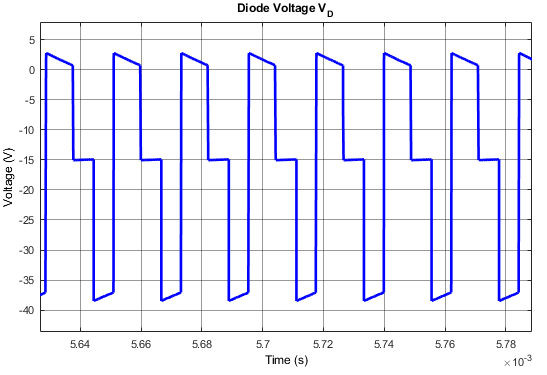
\includegraphics[width=0.7\textwidth]{figures/V_D_48.png}
\caption{Diode Voltage Waveform of the Flyback Converter}
\label{fig:diode48}
\end{center}
\end{figure}

It is observed that the maximum reverse voltage across the diode is around -40V. The selected commercial diode model has a peak repetitive reverse blocking voltage rating of 100V. This result shows that the selected diode is able to operate properly under these steady-state conditions.

During the on (closed) period of the MOSFET switch of the Flyback Converter, the diode is off, and hence not conducting. The reverse voltage over the diode is equal to the negative sum of the output voltage $V_o$ and the secondary side terminal voltage of the transformer $V_2$. During the on (closed) period of the MOSFET switch, the primary side voltage of the transformer, $V_1$, is equal to the source voltage, which is 48V. Then, the secondary side voltage of the transformer during that period is equal to 24V since the transformer has a turns ratio of 2:1 from its primary to secondary ($N_P/N_S = 2$).

$$ V_1 = 48V $$

$$ V_2 = V_1\frac{N_S}{N_P} = 48\times\frac{5}{10} = 24V $$

Then, the reverse voltage over the diode is computed as -39V during that period.

$$ V_{diode} = - V_2 - V_{out} = -24-15 = -39V $$

When the MOSFET switch turns off, the stored magnetic energy in the magnetizing inductor is transferred to the secondary side (load side) of the transformer. Hence, the diode is on until the magnetizing inductance current drops down to 0A. Therefore, the diode voltage is equal to the forward voltage drop of the selected diode, which is equal to 0.7V, during that period. When the magnetizing inductance current becomes zero, the primary side terminals of the transformer is like short circuited with zero voltage. Hence, the secondary side terminals of the transformer is also short circuited. As a result, the diode turns off, and gets out of conduction when the magnetizing inductor current becomes zero. This means that the reverse voltage across the diode is equal to the negative of the output voltage, which is -15V. Therefore, the reverse voltage across the diode becomes -15V after the magnetizing inductance current becomes zero. The reverse diode voltage stays at -15V until the next switching cycle begins with the MOSFET switch turning on (closed) again. When the MOSFET switch is turned on (closed), the reverse voltage across the diode becomes -39V, again as explained above. This operation repeats itself in every switching period.

In short, we observe that the reverse diode voltage is equal to the negative of the output voltage, which is -15, during the time periods when the magnetizing inductance current is equal to zero (0A). This result also shows that the Flyback Converter circuit is operating in DCM mode for the source voltage of 48V.

The snubber circuit voltage and current waveforms of the Flyback Converter circuit are shown in Figure \ref{fig:snubber48}, below.

\begin{figure}[H]
\begin{center}
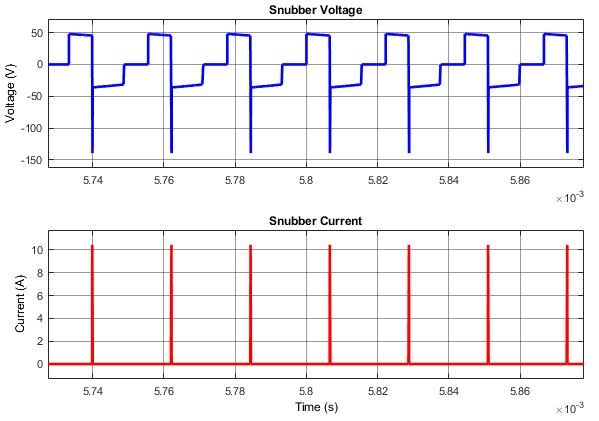
\includegraphics[width=0.7\textwidth]{figures/snubber_48.png}
\caption{RCD Snubber Voltage and Current Waveforms of the Flyback Converter}
\label{fig:snubber48}
\end{center}
\end{figure}

The input current waveform of the Flyback Converter circuit is shown in Figure \ref{fig:Iin48}, below.

\begin{figure}[H]
\begin{center}
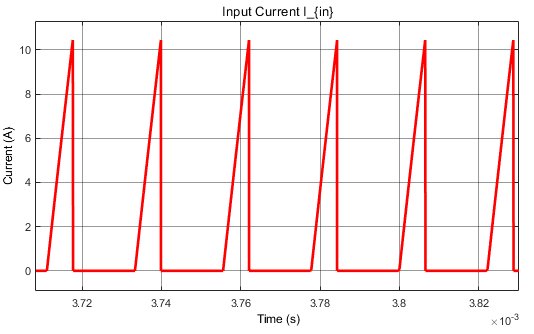
\includegraphics[width=0.7\textwidth]{figures/Iin_48.png}
\caption{Input Current Waveform of the Flyback Converter}
\label{fig:Iin48}
\end{center}
\end{figure}

The input current has a peak of approximately 11A in steady-state operation. The average input current is equal to 1.553A.

The Table \ref{tab:sim48} below shows the average voltage, current and power values obtained from the simulations of the Flyback Converter circuit with $V_{in} = 48V$. 

\begin{table}[H]
    \centering
    \caption{Average Voltage, Current and Power Values Obtained from Simulation}
    \begin{tabular}{|c|c|c|c|c|c|}
    \hline
\textbf{Paremeter}   & \textbf{Value}          & \textbf{Parameter}      & \textbf{Value}          & \textbf{Parameter} & \textbf{Value}         \\ \hline
$V_{in}$ & 48V & $I_{in}$ & 1.553A & $P_{in}$ & 74.56W \\ \hline
$V_{out}$ & 15.04V & $I_{out}$ & 4.01A & $P_{out}$ & 60.31W \\ \hline
$I_D$ & 4.011A & $I_{FET}$ & 1.549A & $\eta$ & 81\% \\ \hline
$V_{out(max)}$ & 15.25V & $V_{out(min)}$ & 14.81V & $\Delta V_{out}$ & 0.44V \\ \hline
    \end{tabular}
    \label{tab:sim48}
\end{table}

Then, the efficiency of the Flyback Converter circuit for the input voltage $V_{in} = 48V$ is obtained as follows:

\begin{align}
    Efficiency = \eta = \frac{P_{out}}{P_{in}}
    \label{eqn:eff48}
\end{align}

$$ Efficiency = \eta = \frac{60.31W}{74.56W} = 0.81\;(81\%) $$

Hence, it is seen from the simulations of the non-ideal Flyback Converter circuit in Simulink that it has an efficiency of around 81\% for the source voltage of 48V. This efficiency level is satisfactory considering that all possible non-idealities in the converter circuit components are included in the simulation model except for the core losses of the designed transformer. 

The detailed efficiency analysis of the Flyback Converter circuit including the core losses of the designed transformer is presented in the Efficiency Analysis section of the report.

It is also observed from Table \ref{tab:sim48} that the output voltage ripple $\Delta V_{out}$ is equal to 0.44V, which is less than the project limitations of 0.6V (4\% of the output average voltage). This result shows that the designed Flyback Converter circuit is able to meet the project specifications  defined on the output voltage limitations successfully.

$$ \Delta V_{out} = 0.44V < 0.60V $$
\section{Component Selection}

\subsection{Analog Controllers \& Components}

We are utilizing a single analog controller in the project for a highly flexible, efficient and feature-packed converter. The main controller selected for these operations is UCC28740 Constant-Voltage Constant-Current Flyback Controller
Using Optocoupled Feedback by Texas Instruments. It will be powered by an auxiliary winding wound to the transformer. It is designated to be always used in DCM operation. It can take feedback from both primary and secondary sides and can keep output voltage constant and performs well in load and line regulation aspects. It has an embedded MOSFET driver to save space lower the component count. Furthermore, its internal algorithm also provides soft-switching to lower the initial stresses on the components.

This controller IC is directly designed by Texas Instruments to control the isolated Flyback Converters. It provides Constant-Voltage (CV) using an optical coupler to improve transient response to large load steps. It also accomplishes Constant-Current (CC) regulation through Primary-Side-Regulation (PSR) techniques. It processes the information taken from opto-coupled feedback and the auxiliary flyback winding, and uses this processed information to achieve precise high-performance control of the output voltage and current of the converter. The control algorithms used in this IC helps it to achieve high efficiency levels. The DCM operation with the valley switching technique reduces the switching losses, and hence increases the overall efficiency.

The selected controller has a maximum switching frequency of 100 kHz, and always maintains the control of the peak primary current in the transformer. Furthermore, the embedded protection features help to keep the primary and secondary component stresses of the converter in check.

A reference design schematic for the selected controller IC UCC28740 is shown in Figure \ref{fig:analog_cont}, below.

\begin{figure}[H]
\centering
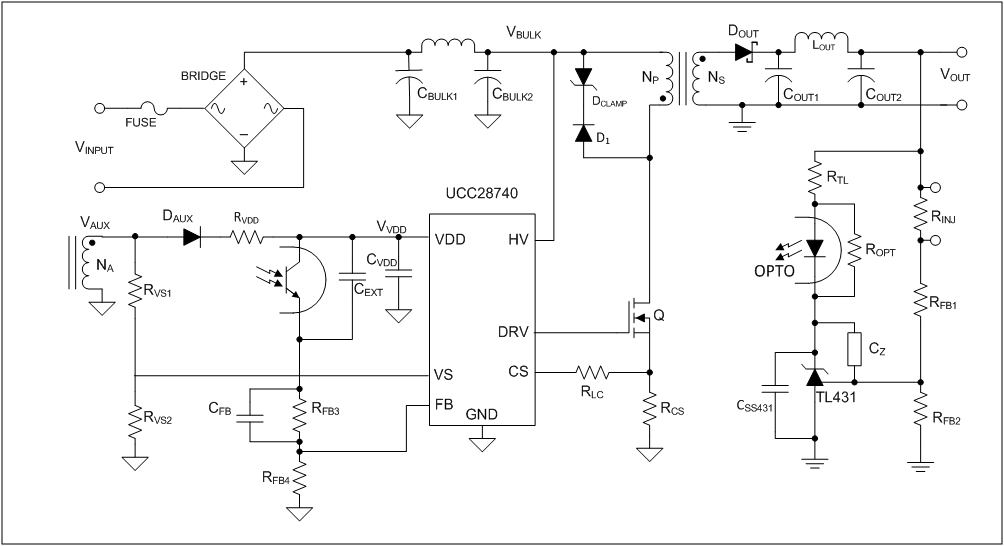
\includegraphics [width=0.8\textwidth]{figures/Analog_Controller.png}
\caption{Flyback Controller Reference Design with UCC28740}
\label{fig:analog_cont}
\end{figure}

\subsection{MOSFET Selection}
For the MOSFET selection, we need to consider the maximum voltage and current stresses over the MOSFET.

The maximum voltage stress over the MOSFET is obtained analytically by the following relation.

$$ V_{sw,peak} = V_{in,max} + \frac{N_P}{N_S}V_{out} $$

where $ V_{in,max} = 48\;V $, $ V_{out} = 15\;V $ and $ \frac{N_P}{N_S} = 1.9 $.

Then, the peak voltage over the MOSFET is computed analytically as follows:

$$ V_{sw,peak} = 48 + 1.9*15 = 76.5\;V $$

This value is in parallel with the peak voltage value obtained from the simulations of the ideal Flyback Converter circuit in Simulink.

The maximum current stress over the MOSFET is obtained analytically by the following relation.

$$ I_{sw,peak} = \frac{1}{(1-D)}\frac{N_S}{N_P}I_o + \frac{N_P}{N_S}\frac{(1-D)T_s}{2L_m}V_o $$

where $ I_o = \frac{P_o}{V_o} = \frac{60}{15} = 4\;A $

Then, the peak MOSFET current is found as follows:

$$ I_{sw,peak} = \frac{1}{(1-0.26)}*\frac{1}{1.9}*4 + 1.9*\frac{(1-0.26)*(1/45000)}{2*28.67*10^{-6}}*15 = 11\;A$$

One thing to notice here is that this peak current is computed assuming CCM operation. However, in our design, the converter mostly operates in DCM as seen from the voltage and current figures presented in the Simulation Results part. Therefore, for the MOSFET peak current value, we need to rely on the simulation results.

However, due to the leakage inductance of the designed transformer, the voltage and current stress over the MOSFET increases. The leakage inductance of the primary winding of the transformer causes voltage spikes over the MOSFET due to the instant changes in inductor current, $di_L/dt$, which in result causes switch failures. In order to prevent giving undesirable damages to the MOSFET, we designed an RCD snubber to provide a safe discharging path for the transformer primary leakage inductance over itself and RC circuit of the snubber. 

From the simulations of the Flyback Converter circuit in Simulink, the MOSFET peak voltage and current are measured as $ V_{sw,peak} = 300\;V $ $ I_{sw,peak} = 10\;A $

Overall, the peak voltage and current ratings for the MOSFET are found as follows:

$$ V_{sw,peak} = 300\;V $$
$$ I_{sw,peak} = 10\;A $$
$$ I_{sw,mean} = 2.84\;A $$
$$ I_{sw,RMS} = 4.366\;A $$

The selected MOSFET should also be able to handle the switching frequencies as high as 45 kHz. 
Since it is a very commonly used value, choosing a 400V MOSFET is reasonable. STP17NK40ZFP by STMicroelectronics is a good choice since it has current rating of 15A continuous, has a low ON resistance and costs relatively low.

\textbf{Selected Switch: } \href{https://pdf1.alldatasheet.com/datasheet-pdf/view/24337/STMICROELECTRONICS/STP17NK40ZFP.html}{STP17NK40ZFP}

Some important parameters for the selected switch are as follows:

\textbf{Switch Parameters}

\begin{itemize}
    \item $V_{DS} = 400V$
    \item $I_{DS} = 15A\;(@\; T_C = 25\degree C)$
    \item $I_{DS} = 9.4A\;(@\; T_C = 100\degree C)$
    \item $R_{DS_{(on)}} = 0.25\ohm\;(max)$
    \item $V_{GS(th)} = 3.75V\;(typ.)$
    \item Diode Forward Voltage: $V_{SD,forward} = 1.6V$\;(max)
    \item Diode Forward Current: $I_{SD} = 15A$
    \item Price: 3.34\$
\end{itemize}

\subsection{Diode Selection}
Similar to the MOSFET selection, the maximum voltage and current stresses over the diode must be determined for the diode selection.

The maximum reverse voltage across the diode during its off period can be calculated as
\begin{align*}
    V_D=V_{out}+N_{PS}V_{in,max}=-40.26V
\end{align*}

It is observed to be $ V_{diode,peak} = -40.26\;V $ from the simulations.

The maximum forward current through the diode during its on period can be calculated as:
\begin{align*}
    I_{s,peak}=\frac{2P_{out}}{D_{MAG}V_{OUT}}=18.89A
\end{align*} 

It is observed to be $ I_{diode,peak} = I_{s,peak} = 19.89\;A $ from the simulations.

Overall, the peak voltage and current ratings for the diode are found as follows:

$$ V_{diode,peak} = -40.26\;V $$
$$ I_{diode,peak} = 19.89\;A $$
$$ I_{diode,mean} = 4.019\;A $$
$$ I_{diode,RMS} = 7.30\;A $$

Also, it should be noted that the average current of the diode will be equal to the average output current, which is 4A. Therefore, MBR10100G from ON Semiconductor is chosen which is a Fast Recovery Schottky diode with 100V and 10A continuous voltage and current ratings diode, which is quite suitable for the given converter application, and the rated operation of our Flyback Converter circuit.

\textbf{Selected Diode: } \href{https://www.onsemi.com/pub/Collateral/MBR1080-D.PDF}{MBR10100G}

Some important parameters for the selected diode are as follows:

\textbf{Diode Parameters}

\begin{itemize}
    \item Type: Schottky Barrier
    \item $V_{RRM} = 100V$
    \item $I_{F(AV)} = 10A\; (@\; T_C = 133\degree C)$
    \item $I_{FRM} = 20A\; (@\; T_C = 133\degree C)$
    \item $I_{FSM} = 150A$
    \item $I_{RRM} = 0.5A$
    \item $V_F = 0.7V\;(@\;i_F = 10A,\; T_C = 125\degree C)$
    \item $I_R = 6mA$
    \item $T_J = -65\;to\;+175\degree C$
    \item $R_{\theta JC} = 2.0\degree C/W$
    \item $R_{\theta JA} = 60\degree C/W$
    \item $R_{ON} = 0.1\ohm\;(@\;i_F = 4A,\;T_C = 150\degree C)$
    \item Price: 0.85\$
\end{itemize}

\subsection{Output Capacitor Selection}
The average voltage across the output capacitor is equal to the average output voltage.

$$ V_{cap,avg} = V_{out} = 15\; $$

Then, the rated voltage of the selected capacitor must be greater than 15 V.

$$ V_{cap,rated} > 15\;V $$

One another limitation on the capacitor selection is the peak-to-peak output voltage ripple limit of the project. The peak-to-peak output voltage ripple is required to be less than 4\%.

$$ \frac{\Delta V_o }{V_o} = 0.04\;(4\%) $$

Then, the maximum allowable output voltage ripple is found as:

$$ \Delta V_o = 0.04*15\;V = 0.6\;V $$ 

Also, let's calculate the maximum allowable ESR for the required ripple.
\begin{align*}
    ESR_{C_{OUT}}=\frac{0.9V_ripple}{I_{s,max}}=20m\Omega
\end{align*}
The output voltage ripple for the Flyback Converter topology is computed from the following relation.

$$ \frac{\Delta V_o }{V_o} = \frac{DT_s}{RC} = \frac{D}{RCf_s} $$

Then, the minimum required output capacitance value is obtained as follows:

$$ C_{min} = \frac{D}{0.04*R*f_s} $$

where $ R = \frac{V_o^2}{P_o} = \frac{15^2}{60} = \frac{225}{60} = 3.75\;\ohm $

$$ C_{min} = \frac{0.26}{0.04*3.75*45000} = 77.8\;\micro F $$

Also, let's calculate the maximum allowable ESR for the required ripple.

\begin{align*}
    ESR_{C_{OUT}}=\frac{0.9V_ripple}{I_{s,max}}=20m\Omega
\end{align*}

We need to select an output capacitor with a rated voltage above 15 V and capacitance value higher than 77.8 \micro F. In addition, the ESR rating of the selected capacitor should also be as small as
possible in order to minimize the voltage drop in the average output voltage level. It is also required to have a small ESR value capacitor in order to keep the converter efficiency as high as possible by minimizing the losses.

Since it is either hard to find or very costly, using ceramic capacitors is not reasonable. Instead, using electrolytic capacitor is a good idea. However, since ESR generally increases with lower capacitance a good balance needs to be found.

Ceramic capacitors are a good choice since their ESR value are quite small compared to aluminum electrolytic capacitors. But, they have the drawback of generally having much higher prices than the aluminum electrolytic capacitors.This creates the compromise or the trade-off between the two types of capacitors. However, since it is difficult to find a small capacitor with the required capacitance value, which is also able to carry the given output current ripple, we decided to use a small aluminum electrolytic capacitor with small ESR rating. It is easier to find small ESR rated aluminum electrolytic capacitors with small capacitance values, which are also able to carry high ripple current values.

Therefore, we decided to select the EEE1HA211P part numbered aluminum electrolytic capacitor (SMD type) of Panasonic. Its rated voltage and current values meets the specifications of our Flyback Converter circuit.

\textbf{Selected Capacitor: } \href{https://media.digikey.com/pdf/Data\%20Sheets/Panasonic\%20Electronic\%20Components/S_Series,Type_V_Rev2018.pdf}{EEE1HA221P}

Some important parameters for the selected capacitor are as follows:

\textbf{Capacitor Parameters}

\begin{itemize}
    \item Type: Aluminum Electrolytic
    \item Rated Capacitance: 220 \micro F
    \item Rated Voltage: $V_{RATED}$ = 50 V
    \item Ripple Current: 300 mA r.m.s.
    \item ESR value: $R_{ESR} = 20m\ohm$
    \item Price: 0.62\$
\end{itemize}

From the simulations of the converter circuit in Simulink with the chosen output capacitor, the output voltage ripple is observed to be approximately 0.4 V, which is lower than the maximum allowable output voltage ripple value of 0.6 V, as computed above.

The peak to peak current ripple on the output capacitor is also obtained from simulations of the converter circuit in Simulink with the chosen capacitors used. The peak to peak current ripple on the output capacitor is observed to be approximately 19.92 A.
\section{Efficiency Analysis}

In this part, efficiency analysis of the flyback converter is done. Efficiency analysis is done under two part. Firstly, analytically efficiency calculation is done by considering non-idealities. There are losses due to non idealities of the system. These losses are caused by, MOSFET $R_{DS}$ resistance, MOSFET rise and fall time (switching losses), diode $R_{ON}$ resistance, transformer cable, capacitor ESR, transformer core. Then, efficiency of the system is obtained from realistic simulation results. There are some differences between analytical calculations and simulation results. These differences will be observed and discussed in this part.

\subsection{Analytically Efficiency Analysis}
 
 Output power of the system is around 60 W. Input power of the system will be changed by input voltage and system losses. System losses of the system is directly affected by input voltage. Specially primary side of the transformer directly is directly affected by input voltage. So, MOSFET losses and transformer cable losses is directly changed with input voltage. In this part, analytically losses will be calculated for different input voltage values, 24 V (minimum input voltage), 36 V( optimal input voltage) and 48 V (maximum input voltage). Loss calculation formulas of system are given below for each component.
 
 MOSFET losses are caused by $R_{DS}$ and switching ;
 
 \begin{align}
     P_{FET} = R_{DS_on}\times I_{FET_{RMS}}^2\\
     P_{SW} = V_{FET_{RMS}}\times I_{FET_{RMS}} \frac{t_{rise}+t_{fall}}{2}\times f_{sw} 
 \end{align}
 
 Diode losses are caused by $R_{ON}$; 
 
 \begin{align}
     P_{diode} = R_{ON}\times I_{D_{RMS}}^2
 \end{align}
 
 Capacitor ESR loss ;
 
 \begin{align}
     P_{cap,ESR} = R_{ESR} \times I_{CAP}^2 \\
     I_{CAP} =  C \frac{dV_{OUT}}{dt} = C\frac{\Delta V_{OUT}}{T}= C \Delta V_{OUT} \times f_{sw} 
 \end{align}
 
 Transformer cable losses ;
 
 \begin{align}
     P_{pri,cable} = R_{AC,pri} \times I_{pri,RMS}^2 \\
     P_{sec,cable} = R_{AC,sec} \times I_{sec,RMS}^2 \\
 \end{align}
 
 Transformer core loss can be found by core properties. Kool Mu 2510 E core parameters to calculate core loss density are given below ;\\
 
$a\ =\ 62,65$\\
$b\ =\ 0.95$\\
$c\ =\ 2.022$\\
$B\ =\ 0.95\ Tesla$\\
$f_{sw}\ =\ 45\ kHZ$\\

Core loss density of Kool Mu cores are given below;
  \begin{align}
     P_f = a\times B^b \times f_{sw}^c\ mW/cm^3
 \end{align}
 
 Volume of the chosen core is 1.87 $cm^3$.  
 
 There are given calculation of required voltage and current RMS calculation.
 
 \begin{align}
    I_{FET,RMS} = \frac{V_{in} D^2 T}{2 L_m}\\
    V_{FET} = V_{in} \\
    I_{D,RMS} = I_{OUT,RMS} 
\end{align}
 
\subsubsection{Analytically Efficiency Analysis for $V_{in}$ = 24 V }

At 24 V input voltage, there is required $I_{FET,RMS}$ and $V_{FET,RMS}$ value for 24 V.\\

$V_{FET} = 24\ V$\\
$I_{FET,RMS}= 5.3\ A$\\
$I_{D,RMS} = 7.3 A $\\

MOSFET losses;

\begin{align}
     P_{FET} = 0.25 \ohm \times 5.3^2\\
     P_{FET} = 7.0225 W \\
     P_{SW} = 24\ V\times 5.3\ A \frac{\frac{(23+13)\times 10^{-9}}{2}}{2}\times 45000 \\
     P_{SW} = 0.11\ W
\end{align}

Diode loss;

\begin{align}
 P_{diode} = 0.1 \ohm \times 7.3 ^2 \\
 P_{diode} = 5.33\ W
\end{align}

Capacitor loss;

\begin{align}
     I_{CAP} =  220\times 10^{-6} \times 45000 \times 0.41 \\
     I_{CAP} = 4.05\ A\ \\
     P_{cap,ESR} = 0.02 \times 4.05^2 \\
     P_{cap,ESR} = 0.33\ W     
\end{align}

Cable loss;

 \begin{align}
     P_{pri,cable} = 0.00278 \times 4.9^2 \\
     P_{pri,cable} = 0.07\ W     \\
     P_{sec,cable} = 0.00139 \times 9.8^2 \\
     P_{sec,cable} = 0.135\ W
 \end{align}
 
 Core loss is same for different input voltages. Core loss depends on core properties, switching frequency and working magnetic flux density. These values are same for all input voltages. That can be differences in practical case because of temperature changes. Cable losses are different for different input values. Under long term working conditions, these temperature changes can create  different core losses. 
 
 Core loss;

 \begin{align}
     P_f = 62.65\times 0.95^2.022 \times 45^1.05\ mW/cm^3\\
     P_f = 3074.34\ mW/cm^3 \\
     P_{core} = 3.07434 \times 1.87 = 5.75\ W
 \end{align}
 
 Total loss of the system when the input voltage is 24 V is ;
 
 \begin{align}
    P_{LOSS}= P_{FET} + P_{SW} + P_{diode} + P_{cap,ESR} + P_{pri,cable} + P_{sec,cable} + P_{core} \\
    P_{LOSS} = 7.0225 + 0.11 + 5.33 + 0.33 + 0.07 + 0.135 + 5.75 \\
    P_{LOSS} = 20.75\ W 
 \end{align}
 
 Efficiency ;
 
 \begin{align}
     \eta = \frac{P_{OUT}}{P_{OUT}+P_{LOSS}}\\
     \eta = \frac{60}{60+20.75} = \frac{60}{80.75} = 0.743 
 \end{align}
 
 To compare analytical results with the simulation results, core loss of the transformer will be ignored, because there is no core losses in the simulations. 
 
 \begin{align}
     P_{without_coreloss} = 15.75\W \\
     \eta = \frac{60}{60+15.75} = \frac{60}{75.75} = 0.792 
 \end{align}
 
 
 \subsubsection{Analytically Efficiency Analysis for $V_{in}$ = 36 V }

At 36 V input voltage, there is required $I_{FET,RMS}$ and $V_{FET,RMS}$ value for 36 V.\\

$V_{FET} = 36\ V$\\
$I_{FET,RMS}= 3.6\ A$\\
$I_{D,RMS} = 7.1 A $\\

MOSFET losses;

\begin{align}
     P_{FET} = 0.25 \ohm \times 3.6^2\\
     P_{FET} = 3.24 W \\
     P_{SW} = 36\ V\times 3.6\ A \frac{\frac{(23+13)\times 10^{-9}}{2}}{2}\times 45000 \\
     P_{SW} = 0.105\ W
\end{align}

Diode loss;

\begin{align}
 P_{diode} = 0.1 \ohm \times 7.1 ^2 \\
 P_{diode} = 5.04\ W
\end{align}

Capacitor loss;

\begin{align}
     I_{CAP} =  220\times 10^{-6} \times 45000 \times 0.44 \\
     I_{CAP} = 4.36\ A\ \\
     P_{cap,ESR} = 0.02 \times 4.36^2 \\
     P_{cap,ESR} = 0.38\ W     
\end{align}

Cable loss ;

 \begin{align}
     P_{pri,cable} = 0.00278 \times 3.8^2 \\
     P_{pri,cable} = 0.04\ W     \\
     P_{sec,cable} = 0.00139 \times 7.6^2 \\
     P_{sec,cable} = 0.08\ W
 \end{align}
 
 \begin{align}
     P_f = 62.65\times 0.95^2.022 \times 45^1.05\ mW/cm^3\\
     P_f = 3074.34\ mW/cm^3 \\
     P_{core} = 3.07434 \times 1.87 = 5.75\ W
 \end{align}
 
 Total loss of the system when the input voltage is 36 V is ;
 
 \begin{align}
    P_{LOSS}= P_{FET} + P_{SW} + P_{diode} + P_{cap,ESR} + P_{pri,cable} + P_{sec,cable} + P_{core} \\
   P_{LOSS} = 3.24 + 0.105 + 5.04 + 0.38 + 0.04 + 0.08 + 5.75 \\
    P_{LOSS} = 17.635\ W 
 \end{align}
 
 Efficiency ;
 
 \begin{align}
     \eta = \frac{P_{OUT}}{P_{OUT}+P_{LOSS}}\\
     \eta = \frac{60}{60+17.635} = \frac{60}{77.635} = 0.783
 \end{align}
 
 To compare analytical results with the simulation results, core loss of the transformer will be ignored, because there is no core losses in the simulations. 
 
 \begin{align}
     P_{without,coreloss} = 12.885W \\
     \eta = \frac{60}{60+12.885} = \frac{60}{72.885} = 0.81
 \end{align}

 \subsubsection{Analytically Efficiency Analysis for $V_{in}$ = 48 V }

At 48 V input voltage, there is required $I_{FET,RMS}$ and $V_{FET,RMS}$ value for 48 V.\\

$V_{FET} = 48\ V$\\
$I_{FET,RMS}= 3.2\ A$\\
$I_{D,RMS} = 7 A $\\

MOSFET losses;

\begin{align}
     P_{FET} = 0.25 \ohm \times 3.2^2\\
     P_{FET} = 2.56 W \\
     P_{SW} = 48\ V\times 3.2\ A \frac{\frac{(23+13)\times 10^{-9}}{2}}{2}\times 45000 \\
     P_{SW} = 0.124\ W
\end{align}

Diode loss;

\begin{align}
 P_{diode} = 0.1 \ohm \times 7 ^2 \\
 P_{diode} = 4.9\ W
\end{align}

Capacitor loss;

\begin{align}
     I_{CAP} =  220\times 10^{-6} \times 45000 \times 0.48 \\
     I_{CAP} = 4.76\ A\ \\
     P_{cap,ESR} = 0.02 \times 4.76^2 \\
     P_{cap,ESR} = 0.453\ W     
\end{align}

Cable loss ;

 \begin{align}
     P_{pri,cable} = 0.00278 \times 3.2^2 \\
     P_{pri,cable} = 0.028\ W     \\
     P_{sec,cable} = 0.00139 \times 6.4^2 \\
     P_{sec,cable} = 0.057\ W
 \end{align}
 
 \begin{align}
     P_f = 62.65\times 0.95^2.022 \times 45^1.05\ mW/cm^3\\
     P_f = 3074.34\ mW/cm^3 \\
     P_{core} = 3.07434 \times 1.87 = 5.75\ W
 \end{align}
 
 Total loss of the system when the input voltage is 48 V is ;
 
 \begin{align}
    P_{LOSS}= P_{FET} + P_{SW} + P_{diode} + P_{cap,ESR} + P_{pri,cable} + P_{sec,cable} + P_{core} \\
   P_{LOSS} = 2.56 + 0.124 + 4.9 + 0.453 + 0.028 + 0.057 + 5.75 \\
    P_{LOSS} = 15.872\ W 
 \end{align}
 
 Efficiency ;
 
 \begin{align}
     \eta = \frac{P_{OUT}}{P_{OUT}+P_{LOSS}}\\
     \eta = \frac{60}{60+15.872} = \frac{60}{75.872} = 0.795
 \end{align}
 
 To compare analytical results with the simulation results, core loss of the transformer will be ignored, because there is no core losses in the simulations. 
 
 \begin{align}
     P_{without,coreloss} = 10.122W \\
     \eta = \frac{60}{60+10.122} = \frac{60}{70.122} = 0.83
 \end{align}

Efficiency of flyback converter is calculated for different input voltage values. As seen from calculations, when the input voltage is increased, efficiency of the system is also increased. That is because of low input current at higher input voltage. When the output power is constant, to supply same power to the output, source supply less current that is why MOSFET current at the primary side of the converter have less RMS current. Less current mean less power losses due to inertial resistances of the system. Efficiency of the system good enough to work as an flyback converter. Most of the losses causes by MOSFET and diode as seen from calculations. To reduce these losses, new MOSFET and diode can be chosen which have less inertial resistances. Cost of these diodes and MOSFETs are much more expensive. When economical situation is considered, chosen diode and MOSFET is acceptable for our flyback converter design. 

\subsection{Efficiency Analysis from Simulations}

In this part, efficiency analysis of the system will be done from Simulink simulation results. There is non-idealities on the system simulation, such as MOSFET and diode inertial resistances, ESR of the capacitor and cable losses of transformer. Also switching losses of the system can be measured better from simulations.

\subsubsection{Efficiency Analysis from Simulations $v_{in}$ = 24 V}

\begin{figure}[H]
\begin{center}
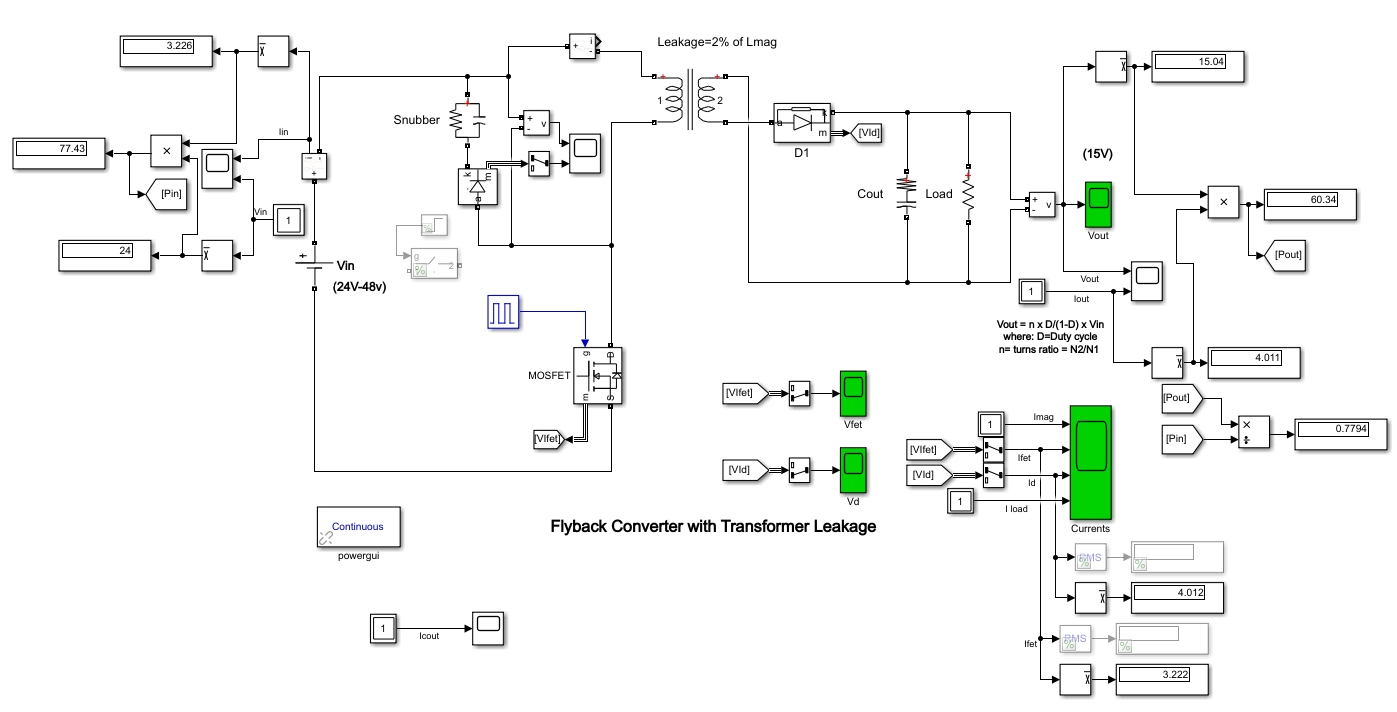
\includegraphics[width=1\textwidth]{figures/24.PNG}
\caption{Efficiency Measurement for 24 V Input Voltage}
\label{fig:eff_24}
\end{center}
\end{figure}

As seen from Figure \ref{fig:eff_24} , efficiency of the flyback converter is 0.779. It is close to the analytical calculations but lower than analytical calculations. At analytical calculations, RMS current and voltage values were calculated by using some approximations. That is why the simulation RMS current and voltage values are different from analytical calculations. So, the efficiency of the system is also measured different because of these differences.There should be additional 5.75 Watt core loss. After core loss is added, efficiency of simulation is given below;

\begin{align}
    \eta = \frac{P_{out}}{P{in}+P_{core}} = \frac{60.34}{77.43+5.75} = \frac{60.34}{83.18} = 0.725
\end{align}
Efficiency of the system is 0.725 when the input voltage is 24.

\subsubsection{Efficiency Analysis from Simulations $v_{in}$ = 36 V}

\begin{figure}[H]
\begin{center}
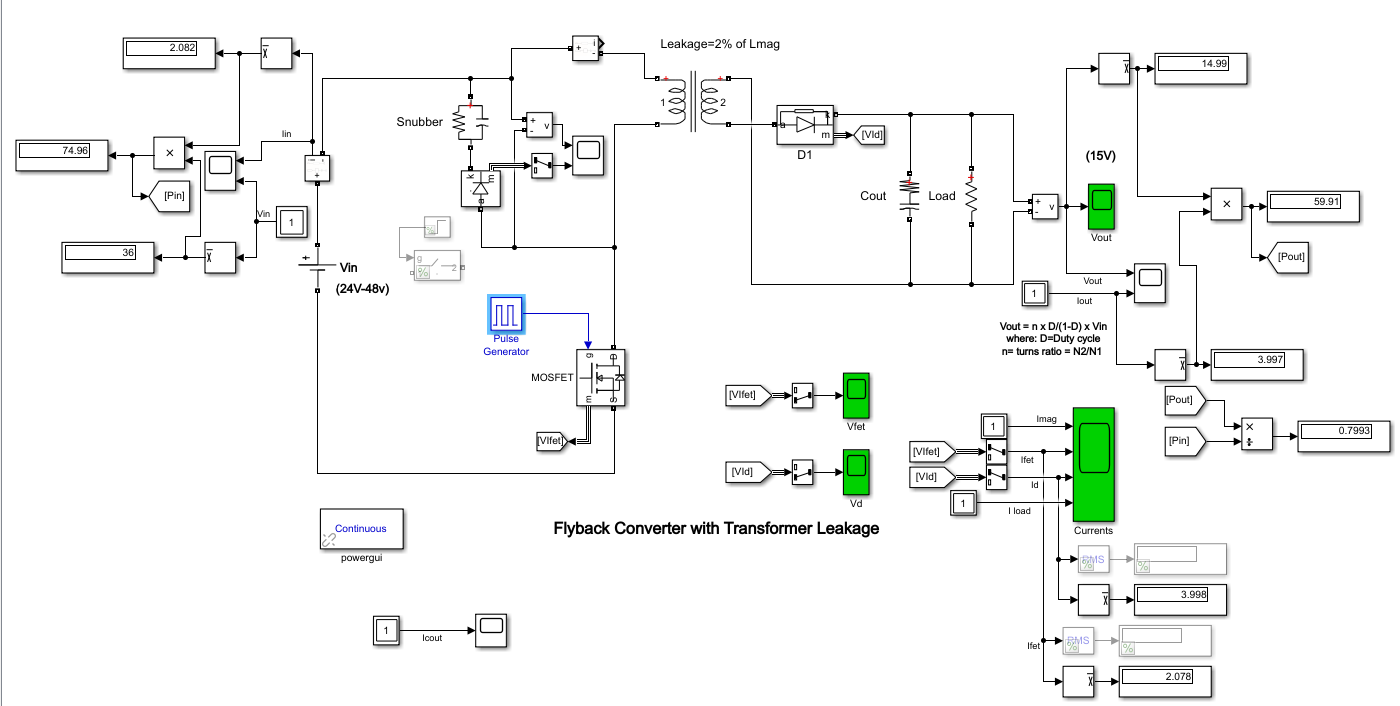
\includegraphics[width=1\textwidth]{figures/36.PNG}
\caption{Efficiency Measurement for 36 V Input Voltage}
\label{fig:eff_36}
\end{center}
\end{figure}

As seen from Figure \ref{fig:eff_36} , efficiency of the flyback converter is 0.799. Which is again so close to the analytical calculations but some differences are observed because of approximations by calculating RMS values.There should be additional 5.75 Watt core loss. After core loss is added, efficiency of simulation is given below;

\begin{align}
    \eta = \frac{P_{out}}{P{in}+P_{core}} = \frac{59.91}{74.96+5.75} = \frac{59.91}{80.71} = 0.742
\end{align}
Efficiency of the system is 0.742 when the input voltage is 36 V.

\subsubsection{Efficiency Analysis from Simulations $v_{in}$ = 48 V}

\begin{figure}[H]
\begin{center}
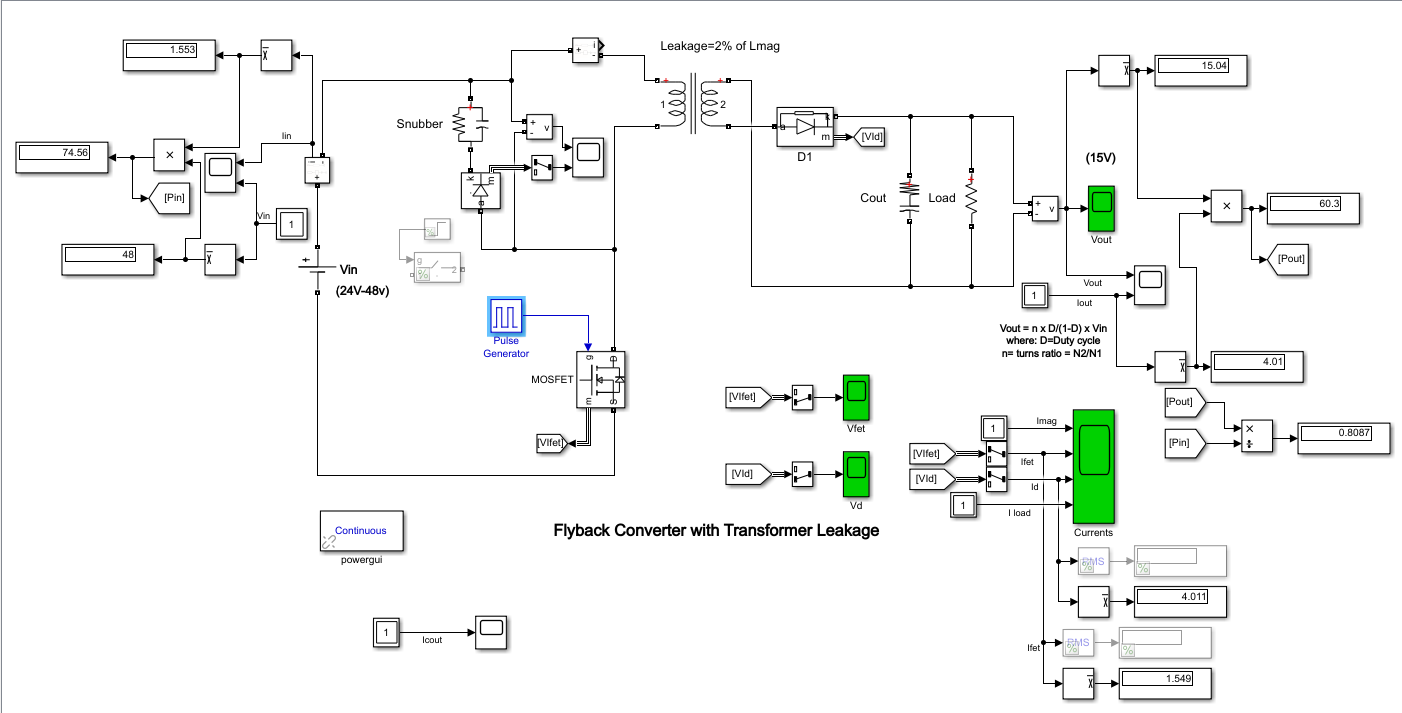
\includegraphics[width=1\textwidth]{figures/48.PNG}
\caption{Efficiency Measurement for 48 V Input Voltage}
\label{fig:eff_48}
\end{center}
\end{figure}

As seen from Figure \ref{fig:eff_48} , efficiency of the flyback converter is 0.808. There should be additional 5.75 Watt core loss. After core loss is added, efficiency of simulation is given below;

\begin{align}
    \eta = \frac{P_{out}}{P{in}+P_{core}} = \frac{60.3}{74.56+5.75} = \frac{60.3}{80.31} = 0.751
\end{align}
Efficiency of the system is 0.751 when the input voltage is 48 V.
As seen from all measurements, efficiency of system is good enough. Most of the losses are caused by MOSFET and diode inertial resistance. These losses can be reduced by using different MOSFET and diodes but chosen components are good enough and economical.


General efficiency analyse comparison is given below;

\begin{table}[H]
\centering
\caption{Efficiency Comparison Table for Analytical Calculations and Simulation Results}
\begin{tabular}{|l|l|l|l|l|}
\hline
Input Voltage & Analytical Efficiency & \begin{tabular}[c]{@{}l@{}}Simulation Efficiency \\ with Core Loss\end{tabular} & \begin{tabular}[c]{@{}l@{}}Analytical Efficiency\\  without Core Lose\end{tabular} & Simulation Efficiency \\ \hline
24 V          & \%74.3                & \%72.5                                                                          & \%79.2                                                                             & \%77.9                \\ \hline
36 V          & \%78.3                & \%74.2                                                                          & \%81                                                                               & \%79.9                \\ \hline
48 V          & \%79.5                & \%76                                                                            & \%83                                                                               & \%81                  \\ \hline
\end{tabular}
\end{table}

\newpage
\section{Thermal Analysis}

As seen from MOSFET and Diode loss calculation, there is required heat sink for MOSFET and Diode to protect components from higher temperature. Diode and MOSFET have typical working temperature. Temperature of these components should be between temperature limitations. Losses of the system is dissipated as heat. This heat can damage our components. There is required electric circuit equivalent of thermal design to do better thermal analysis. Required thermal resistance values can be found from data sheets of diode MOSFET and heat sinks. Electric circuit equivalent of thermal analysis is given Figure \ref{fig:wo-hs}.

\begin{figure}[H]
\begin{center}
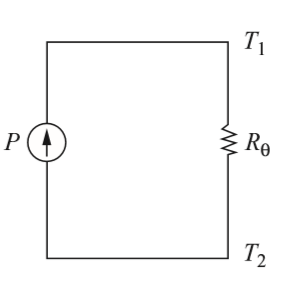
\includegraphics[width=0.4\textwidth]{figures/wo-hs.PNG}
\caption{An Electric Circuit Equivalent of Thermal Analysis without Heat Sink}
\label{fig:wo-hs}
\end{center}
\end{figure}

As seen from Figure \ref{fig:wo-hs}, $R_{\theta}$ is the sum of junction to case thermal resistance and case to ambient thermal resistance which are, $R_{th,j-c}$ and $R_{th,c-a}$. 
$$R_{\theta} = \frac{T_1 - T_2 }{P_{loss}}$$

Equivalent circuit of system is changed after heat sink addition. When there is lower thermal resistance, it means there is lower temperature increases. At Figure \ref{fig:w-hs}, equivalent circuit of thermal analysis with heat sink is given. 

\begin{figure}[H]
\begin{center}
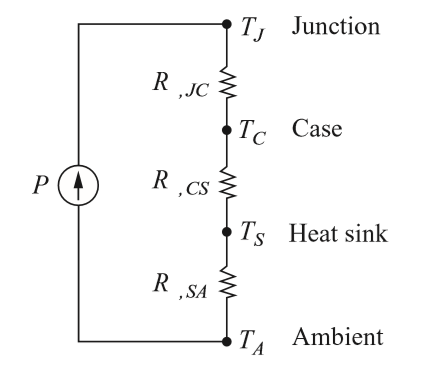
\includegraphics[width=0.5\textwidth]{figures/with hs.PNG}
\caption{An Electric Circuit Equivalent of Thermal Analysis with Heat Sink}
\label{fig:w-hs}
\end{center}
\end{figure}

$R_{,CS}$ and $R_{,SA}$ is  given by manufacturer of the heat sink. Sum of these two thermal resistance is important for thermal analysis and can be found from heat sink data sheet. Thermal design of the converter will be done according to these equivalent circuits.

\subsection{MOSFET Heat Sink Selection}

As seen from efficiency section, there is more power losses on the MOSFET when the input voltage is higher. So, thermal design of the system will be done according to minimum input voltage value. System should be designated for maximum power loss condition. Working temperature of the MOSFET is -55 to 150 \degree C . 125 \degree C is selected to have better thermal design. Maximum limitation of the system is reduced. There should be unexpected situations, that is why 125\degree C is better for limitation. Required parameters and measurements are given below for thermal analysis. Ambient temperature is taken as 25\degree C.

$$R_{thj-c}\ =\ 3.6\ \degree C / W$$
$$R_{thc-amb}\ =\ 62.5\ \degree C / W$$
$$P_{FET} = P_{CON}+P{SW} = 7.0225+0.11 = 7.1325\ W$$

Without heat sink, to reach 125\degree C, required power calculation is given below;

\begin{align}
    P_{Thermal} = \frac{T_1 - T_2}{R_\theta} = \frac{125-25}{62.5+3.6} = 1.513\ W \\
\end{align}

1.513 W is enough to damage our MOSFET. There is power loss more than 1.513 W which is 7.1325 W. To protect our MOSFET, there is required heat sink which will reduce to case to ambient thermal resistance. When this thermal resistance is reduced, there will be less temperature increases under same power loss. Required heat sink thermal resistance calculation is given below;

\begin{align}
    P_{loss} = 7.1325\ W \\
    P_{loss} = \frac{T_1 - T_2 }{R_{final}}\\
    R_{final} = \frac{100}{7.1325} = 14\ \degree C/W
    R_{heat sink} = R_{final} - R_{thj-c} = 14-3.6 = 10.4\ \degree C/W\\
\end{align}

According to calculations, thermal resistance of the heat sink should be lower than 10.4 \degree C/W. When the cost and thermal analysis is done, Assmann WSW Components, V5220L heat sink is chosen. Price of the heat sink is 0.8 \$. 
$$R_{heat sink} = 8.0\ \degree C/W $$

Thermal analysis after heat sink ;

\begin{align}
    P_{loss} = 7.1325 W = \frac{T_{final}-T_{amb}}{R_{final}}\\
    7.1325 W = \frac{T_{final}-25}{8+3.6} \\
    T_{final} = (7.1325 \times 11.6 ) + 25 = 107.8\ \degree C 
\end{align}

MOSFET temperature at maximum loss condition is 107. 8 \degree C . Which is lower than limitation temperature.

\subsection{Diode Heat Sink Selection}

As seen from efficiency calculations, diode power losses are similar for different input voltage due to constant output power. Diode current is like output current. Maximum power loss on diode is shown at 24 V input voltage but so close to other cases. Required parameters and measurements are given below for thermal analysis and design. Diode working temperatıre is between -65 to 175 \degree C. 150  \degree C is chosen as limitation for diode temperature to have better thermal design. 

$$R_{thj-c}\ =\ 2\ \degree C / W$$
$$R_{thc-amb}\ =\ 60\ \degree C / W$$
$$P_{diode}  = 5.33\ W$$

Without heat sink, to reach 150\degree C, required power calculation is given below;

\begin{align}
    P_{Thermal} = \frac{T_1 - T_2}{R_\theta} = \frac{150-25}{60+2} = 2.02\ W \\
\end{align}

2.02 W is enough to damage our diode. There is power loss more than 2.02 W which is 5.33 W. To protect our diode, there is required heat sink which will reduce to case to ambient thermal resistance. When this thermal resistance is reduced, there will be less temperature increases under same power loss. Required heat sink thermal resistance calculation is given below;

\begin{align}
    P_{loss} = 5.33\ W \\
    P_{loss} = \frac{T_1 - T_2 }{R_{final}}\\
    R_{final} = \frac{125}{5.33} = 23.45\ \degree C/W
    R_{heat sink} = R_{final} - R_{thj-c} = 23.4-2 = 21.4\ \degree C/W\\
\end{align}

According to calculations, thermal resistance of the heat sink should be lower than 21.4 \degree C/W. When the cost and thermal analysis is done, CUI Devices- HSS-B20-NP-01 heat sink is chosen for thermal design. Price of the heat sink is 0.2 \$. 
$$R_{heat sink} = 16.29\ \degree C/W $$

Thermal analysis after heat sink ;

\begin{align}
    P_{loss} = 5.33 W = \frac{T_{final}-T_{amb}}{R_{final}}\\
    5.33 W = \frac{T_{final}-25}{16.29+2} \\
    T_{final} = (5.33 \times 18.29 ) + 25 = 122.49\ \degree C 
\end{align}

Diode temperature at maximum loss condition is 122.49 \degree C . Which is lower than limitation temperature(150 \degree C).

\newpage
\section{Bonus: Closed Loop Control of the Flyback Converter}

In this section, we design a compensator for the closed loop control of the Flyback Converter circuit. The design steps are explained in detail in the following subsections. First of all, we start by deriving the small signal ac equivalent circuit model of the Flyback Converter circuit. Then, we obtain the open loop control to output transfer function of the Flyback Converter using the derived small signal ac equivalent circuit model. Finally, the compensator design steps are explained using the derived transfer function, and including the possible non-idealities of the circuit components. Then, the simulation results for the compensated Flyback Converter with the designed compensator are presented at the end of the section in order to see the closed loop performance of the circuit.

\subsection{AC Equivalent Circuit Modeling}

The basic circuit diagram of the Flyback Converter circuit is shown in Figure \ref{com:fly1}, below.

\begin{figure}[H]
\begin{center}
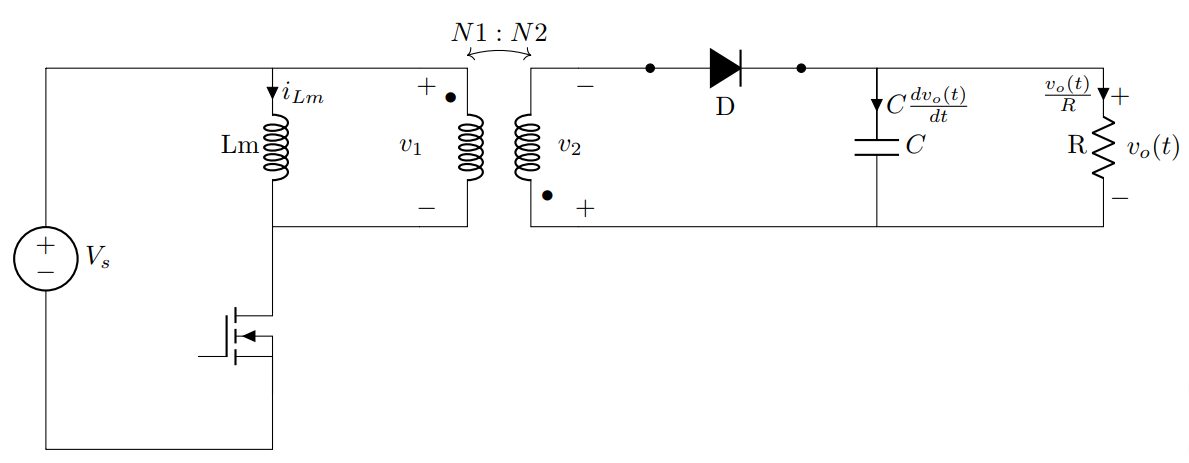
\includegraphics[width=1\textwidth]{Compensator/flyback1.png}
\caption{Flyback Converter Circuit}
\label{com:fly1}
\end{center}
\end{figure}

We start by determining the voltage and current waveforms of the inductor and capacitor.

The converter circuit becomes as shown in Figure \ref{com:fly_on} when the switch is closed for time period of 0 < t < D$T_s$.

\textbf{For 0 < t < D$T_s$:}

\begin{figure}[H]
\begin{center}
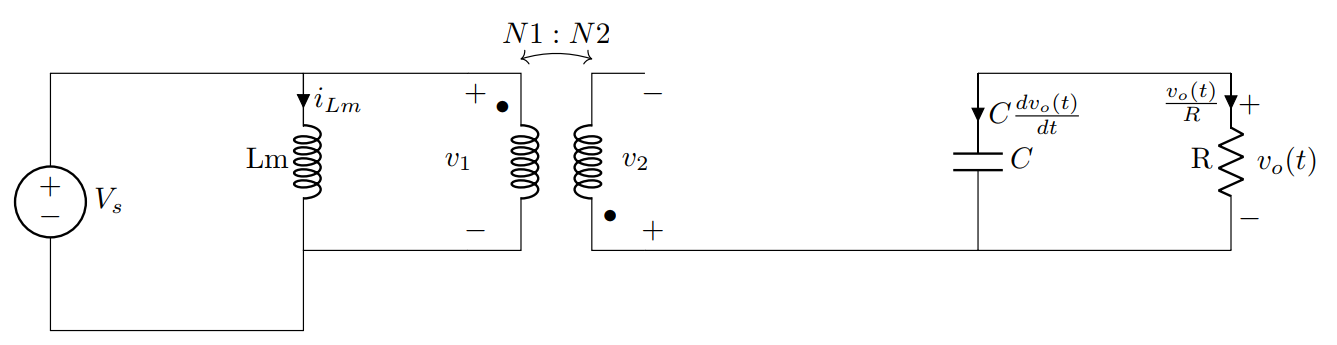
\includegraphics[width=1\textwidth]{Compensator/flyback_on.png}
\caption{Flyback Converter Circuit with the Switch Closed}
\label{com:fly_on}
\end{center}
\end{figure}

Then, the magnetizing inductor voltage equation of the transformer when the switch is closed can be written as follows:

\begin{align}
    v_L(t) = L_m\frac{di_{Lm}(t)}{dt} = v_s(t)
\end{align}

Similarly, the output capacitor current equation when the switch is closed can be written as follows:

\begin{align}
    i_c(t) = C\frac{dv_o(t)}{dt} = -\frac{v_o(t)}{R}
\end{align}

The relation between the input/source current and the magnetizing current is also written as follows when the switch is closed.

\begin{align}
    i_s(t) = i_{Lm}(t)
\end{align}

We can now make the small-ripple approximation. We replace the input voltage signal $v_s(t)$ and the output voltage signal $v_o(t)$ with their low frequency averaged values $\langle v_s(t) \rangle_{T_s}$ and $\langle v_o(t) \rangle_{T_s}$, respectively.

\begin{align}
    v_L(t) = L_m\frac{di_{Lm}(t)}{dt} \approx \langle v_s(t) \rangle_{T_s}
\end{align}

\begin{align}
    i_c(t) = C\frac{dv_o(t)}{dt} \approx -\frac{\langle v_o(t) \rangle_{T_s}}{R}
\end{align}

We can also write the small-ripple approximation of the source current equation by replacing the source current $i_s(t)$ and the magnetizing current $i_{Lm}(t)$ signals with their low frequency averaged values $\langle i_s(t) \rangle_{T_s}$ and $\langle i_{Lm}(t) \rangle_{T_s}$, respectively.

\begin{align}
    i_s(t) \approx \langle i_s(t) \rangle_{T_s} = \langle i_{Lm}(t) \rangle_{T_s}
\end{align}

The converter circuit becomes as shown in Figure \ref{com:fly_off} when the switch is open for time period of D$T_s$ < t < $T_s$.

\textbf{For D$T_s$ < t < $T_s$:}

\begin{figure}[H]
\begin{center}
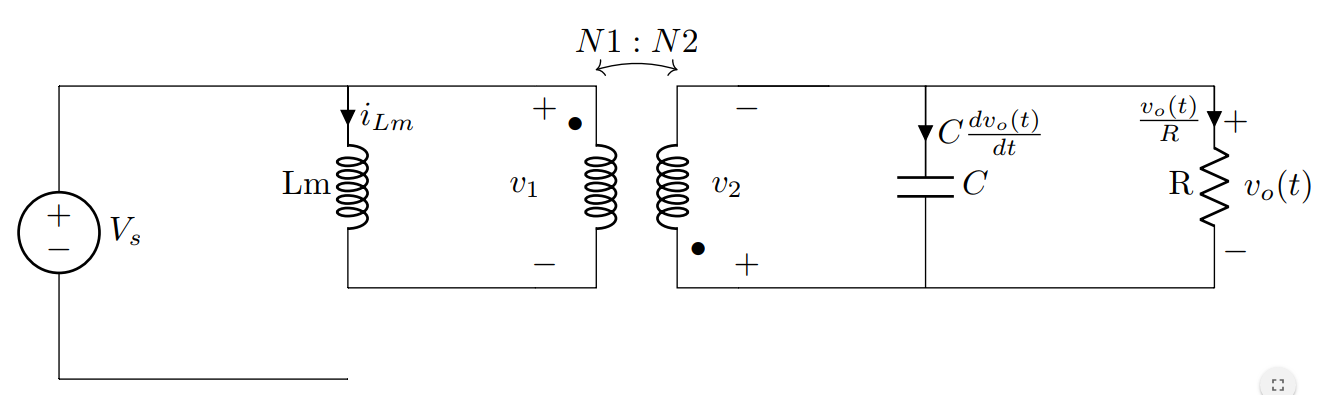
\includegraphics[width=1\textwidth]{Compensator/flyback_off.png}
\caption{Flyback Converter Circuit with the Switch Open}
\label{com:fly_off}
\end{center}
\end{figure}

Then, the magnetizing inductor voltage equation of the transformer when the switch is open can be written as follows:

\begin{align}
    v_L(t) = L_m\frac{di_{Lm}(t)}{dt} = -v_o(t)\frac{N_1}{N_2}
\end{align}

Similarly, the output capacitor current equation when the switch is open can be written as follows:

\begin{align}
    i_c(t) = C\frac{dv_o(t)}{dt} = i_{Lm}(t)\frac{N_1}{N_2} -\frac{v_o(t)}{R}
\end{align}

The input/source current equation is also written as follows when the switch is open. The source current is equal to zero during this time period since the switch is open.

\begin{align}
    i_s(t) = 0
\end{align}

Again, we make the small-ripple approximation. We replace the input voltage signal $v_s(t)$ and the output voltage signal $v_o(t)$ with their low frequency averaged values $\langle v_s(t) \rangle_{T_s}$ and $\langle v_o(t) \rangle_{T_s}$, respectively.

\begin{align}
    v_L(t) = L_m\frac{di_{Lm}(t)}{dt} \approx \langle v_o(t) \rangle_{T_s}\frac{N_1}{N_2}
\end{align}

\begin{align}
    i_c(t) = C\frac{dv_o(t)}{dt} \approx \langle i_{Lm}(t) \rangle_{T_s}\frac{N_1}{N_2} -\frac{\langle v_o(t) \rangle_{T_s}}{R}
\end{align}

We do not need to make the small-ripple approximation for the source current $i_s(t)$ since it is already equal to zero due to open switch during this time period.

\begin{align}
    i_s(t) \approx \langle i_s(t) \rangle_{T_s} = 0
\end{align}

The low frequency average of the inductor voltage is found as follows by using the inductor Volt-Second balance method.

\begin{align}
    \langle v_L(t) \rangle_{T_s} = \frac{1}{T_s}\int_{t}^{t+T_s} v_L(\tau)d\tau \approx d(t)\langle v_s(t) \rangle_{T_s} + d'(t)[-\langle v_o(t) \rangle_{T_s}\frac{N_1}{N_2}]
\end{align}

\begin{align}
    \langle v_L(t) \rangle_{T_s} = L_m\frac{\langle i_{Lm}(t) \rangle_{T_s}}{dt} \approx d(t)\langle v_s(t) \rangle_{T_s} + d'(t)[-\langle v_o(t) \rangle_{T_s}\frac{N_1}{N_2}]
    \label{eqn:ind}
\end{align}

where $d'(t) = 1 - d(t)$.

The low frequency average capacitor current is also found by using the Capacitor Charge Balance method as follows:

\begin{align}
    \langle i_c(t) \rangle_{T_s} = d(t)(-\frac{\langle v_o(t) \rangle_{T_s}}{R}) + d'(t)[\langle i_{Lm}(t) \rangle_{T_s}\frac{N_1}{N_2}-\frac{\langle v_o(t) \rangle_{T_s}}{R}]
\end{align}

\begin{align}
    \langle i_c(t) \rangle_{T_s} = C\frac{d\langle v_o(t) \rangle_{T_s}}{dt} = d(t)(-\frac{\langle v_o(t) \rangle_{T_s}}{R}) + d'(t)[\langle i_{Lm}(t) \rangle_{T_s}\frac{N_1}{N_2}-\frac{\langle v_o(t) \rangle_{T_s}}{R}]
\end{align}

We can simplify this equation as follows:

\begin{align}
    \langle i_c(t) \rangle_{T_s} = C\frac{d\langle v_o(t) \rangle_{T_s}}{dt} = -\frac{\langle v_o(t) \rangle_{T_s}}{R} + d'(t)\langle i_{Lm}(t) \rangle_{T_s}\frac{N_1}{N_2}
    \label{eqn:cap}
\end{align}

Finally, we can write the relation between the input/source current and the magnetizing current with the low frequency small-ripple approximation as follows:

\begin{align}
    \langle i_s(t) \rangle_{T_s} = d(t)\langle i_{Lm}(t) \rangle_{T_s}
    \label{eqn:scurr}
\end{align}

\textbf{Perturbation and Linearization}

These derived equations are non-linear since they involve the multiplication of time-varying quantities. This multiplication of time-varying signals create harmonics, and is a non-linear process. Hence, the next step is to perturb and linearize these equations in order to construct the converter small-signal ac equations.

Assume that we drive the converter at some steady state with $d(t) = D$ and $v_s(t) = V_s$ at a quiescent point. In other words, we assume that the converter source voltage $v_s(t)$ and duty cycle $d(t)$ can be expressed as quiescent values plus small ac variations, as follows:

\begin{align}
     \langle v_s(t) \rangle_{T_s} = V_s + \hat{v}_s(t)
\end{align}

\begin{align}
     \langle d(t) \rangle_{T_s} = D + \hat{d}(t)
\end{align}

In response to these inputs, and after all transients have decayed, the average converter magnetizing current, output voltage and source current waveforms can also be expressed as quiescent values plus small ac variations as follows:

\begin{align}
     \langle i_{Lm}(t) \rangle_{T_s} = I_{Lm} + \hat{i}_{Lm}(t)
\end{align}

\begin{align}
     \langle v_o(t) \rangle_{T_s} = V_o + \hat{v}_o(t)
\end{align}

\begin{align}
     \langle i_s(t) \rangle_{T_s} = I_s + \hat{i}_s(t)
\end{align}

It is also assumed that the ac variations are quite small in magnitude compared to the dc quiescent values.

\begin{align}
    |\hat{v}_s(t)| \ll |V_s|
\end{align}
\begin{align}
    |\hat{d}(t)| \ll |D|
\end{align}
\begin{align}
    |\hat{i}_{Lm}(t)| \ll |I_{Lm}|
\end{align}
\begin{align}
    |\hat{v}_o(t)| \ll |V_o|
\end{align}
\begin{align}
    |\hat{i}_s(t)| \ll |I_s|
\end{align}

Then, we can rewrite the large signal averaged equations in \eqref{eqn:ind}, \eqref{eqn:scurr} and \eqref{eqn:cap} as follows:

\begin{align}
    L_m\frac{d}{dt}(I_{Lm}+\hat{i}_{Lm}(t)) = (D+\hat{d}(t))(V_s+\hat{v}_s(t)) + (D'-\hat{d}(t))(-V_o-\hat{v}_o(t))\frac{N_1}{N_2}
\end{align}

\begin{align}
    C\frac{d}{dt}(V_o+\hat{v}_o(t)) = -\frac{(V_o+\hat{v}_o(t))}{R} + (D'-\hat{d}(t))(I_{Lm}+\hat{i}_{Lm}(t))\frac{N_1}{N_2}
\end{align}

\begin{align}
    I_s + \hat{i}_s(t) = (D+\hat{d}(t))(I_{Lm}+\hat{i}_{Lm}(t))
\end{align}

We can see that all three the inductor voltage, capacitor current and source current equations involve DC terms, first order ac terms (linear) and second order ac terms (non-linear). We can neglect the second order ac terms (non-linear ac terms) thanks to the small-signal assumption which states that the magnitude of the ac variations are quite small compared to the dc quiescent values. This implies that the second order ac terms (non-linear) are quite small in magnitude compared to the first order ac terms (linear) and the DC terms, and hence they can be neglected in the small signal analysis.

Also, by definition, the DC terms on the right-hand side of the above equations are equal to the DC terms on the left-hand side of the equation, or just zero. The equivalence of the DC terms on the right-hand side and the left hand-side of the above equations can be derived from the inductor Volt-Second and capacitor Charge-Balance principles at the steady state operation. 

The equivalence of the DC terms on the right and left hand sides of the above equations for the inductor voltage, capacitor current and source current are given below in equations \eqref{eqn:dc_ind}, \eqref{eqn:dc_cap} and \eqref{eqn:dc_sour}, respectively.

\begin{align}
    0 = DV_s - D'V_o\frac{N_1}{N_2}
    \label{eqn:dc_ind}
\end{align}

\begin{align}
    0 = -\frac{V_o}{R} + D'I_{Lm}\frac{N_1}{N_2}
    \label{eqn:dc_cap}
\end{align}

\begin{align}
    I_s = DI_{Lm}
    \label{eqn:dc_sour}
\end{align}

We obtain the steady state voltage transfer ratio of the ideal Flyback Converter circuit from equation \eqref{eqn:dc_ind} as follows:

\begin{align}
    \frac{V_o}{V_s} = \frac{D}{D'}\frac{N_2}{N_1}
\end{align}

We obtain the average magnetizing inductance current in steady-state operation from equation \eqref{eqn:dc_cap} as follows:

\begin{align}
    I_{Lm} = \frac{1}{D'}\frac{V_o}{R}\frac{N_2}{N_1}
\end{align}

These equations can also be obtained from the analysis of the Flyback Converter circuit under steady-state operation. The above system of equations can be solved to find the quiescent output voltage $V_o$, inductor current $I_{Lm}$ and source (input) current $I_g$ for the given quiescent values of the input voltage $V_s$ and the duty cycle D. Then, the obtained quiescent value results can be inserted into the small-signal ac equations for the linear ac terms, as will be expressed below.

Finally, we are left with the first order linear ac terms. Then, we can write the small signal equations for the inductor voltage, capacitor current and source current as follows by writing the equivalence of the first order linear ac terms on the both sides of the above nonlinear equations.

\begin{align}
    L_m\frac{d\hat{i}_{Lm}}{dt} = D\hat{v}_s(t) + (V_s+V_o\frac{N_1}{N_2})\hat{d}(t) - D'\hat{v}_o(t)\frac{N_1}{N_2}
    \label{eqn:ss_ind}
\end{align}

\begin{align}
    C\frac{d\hat{v}_o}{dt} = -\frac{\hat{v}_o(t)}{R} + D'\frac{N_1}{N_2}\hat{i}_{Lm}(t) - I_{Lm}\frac{N_1}{N_2}\hat{d}(t)
    \label{eqn:ss_cap}
\end{align}

\begin{align}
    \hat{i}_s(t) = D\hat{i}_{Lm}(t) + I_{Lm}\hat{d}(t)
    \label{eqn:ss_source}
\end{align}

After, obtaining the governing small-signal ac equations for the Flyback Converter circuit, we can now construct the corresponding equivalent circuits for the above equations.

The small-signal equivalent circuit for the inductor voltage equation given in \eqref{eqn:ss_ind} is shown in Figure \ref{com:fly_part1} below.

\begin{figure}[H]
\begin{center}
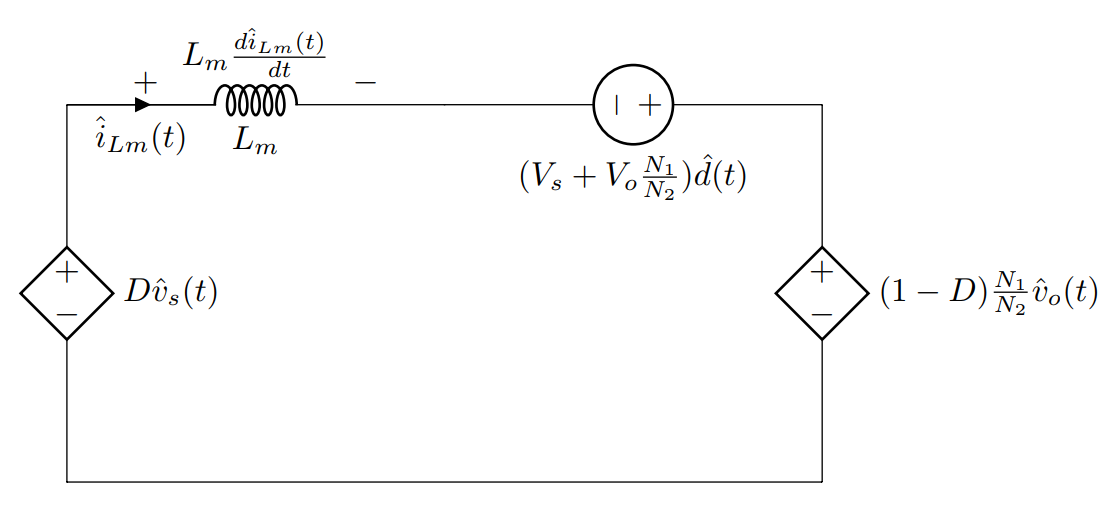
\includegraphics[width=1\textwidth]{Compensator/flyback_part1.png}
\caption{Small-Signal Equivalent Circuit for the Inductor Voltage Equation}
\label{com:fly_part1}
\end{center}
\end{figure}

The small-signal equivalent circuit for the capacitor current equation given in \eqref{eqn:ss_cap} is shown in Figure \ref{com:fly_part2} below.

\begin{figure}[H]
\begin{center}
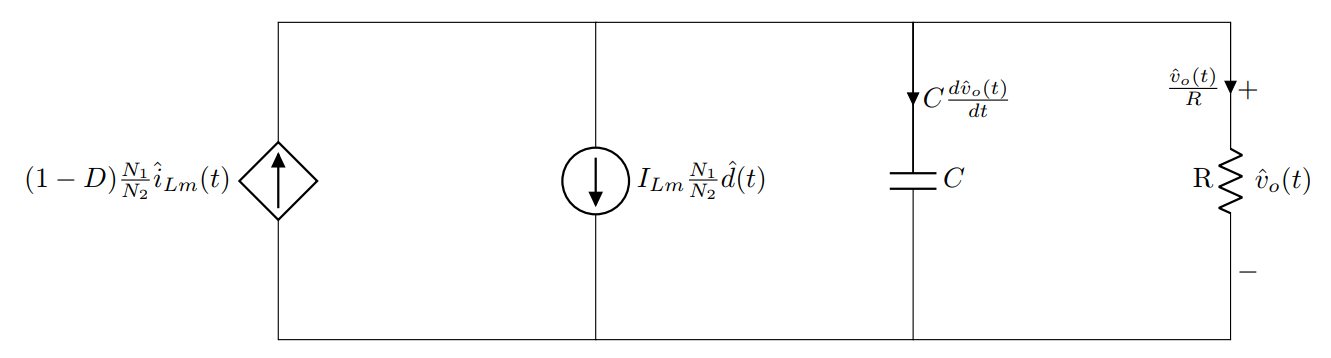
\includegraphics[width=1\textwidth]{Compensator/flyback_part2.png}
\caption{Small-Signal Equivalent Circuit for the Capacitor Current Equation}
\label{com:fly_part2}
\end{center}
\end{figure}

The small-signal equivalent circuit for the source current equation given in \eqref{eqn:ss_source} is shown in Figure \ref{com:fly_part3} below.

\begin{figure}[H]
\begin{center}
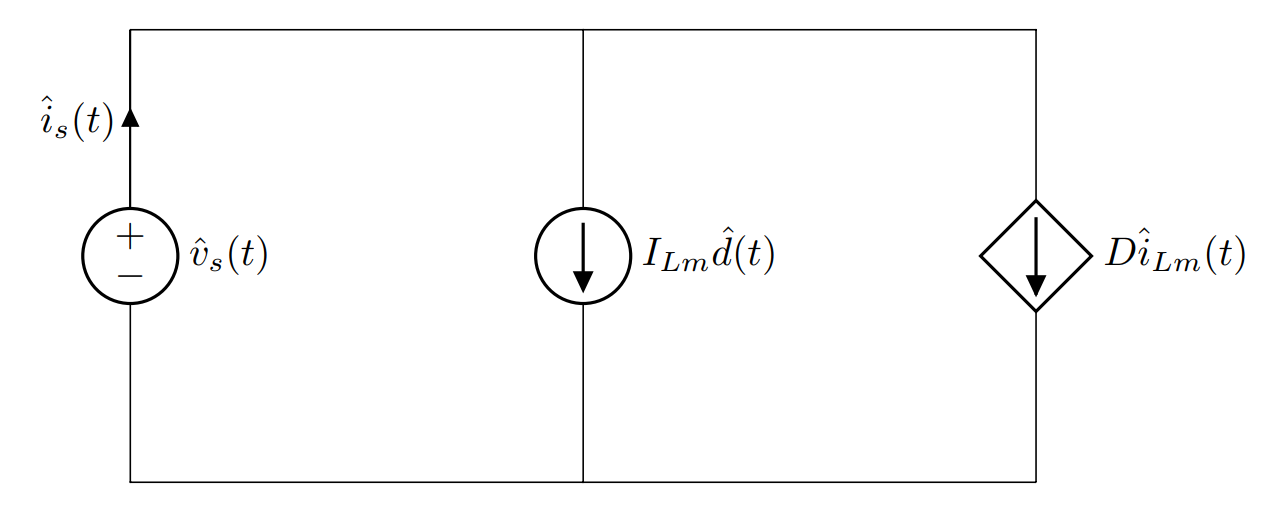
\includegraphics[width=1\textwidth]{Compensator/flyback_part3.png}
\caption{Small-Signal Equivalent Circuit for the Source Current Equation}
\label{com:fly_part3}
\end{center}
\end{figure}

Then small-signal ac circuits given in Fig \ref{com:fly_part1}, \ref{com:fly_part2} and \ref{com:fly_part3} can be combined into a single equivalent circuit by replacing the dependent voltage and current sources in these three circuits with ideal transformers with the relevant turns ratio. The combined equivalent small-signal ac circuit of the Flyback Converter is shown in Figure \ref{com:fly_combined}, below.

\begin{figure}[H]
\begin{center}
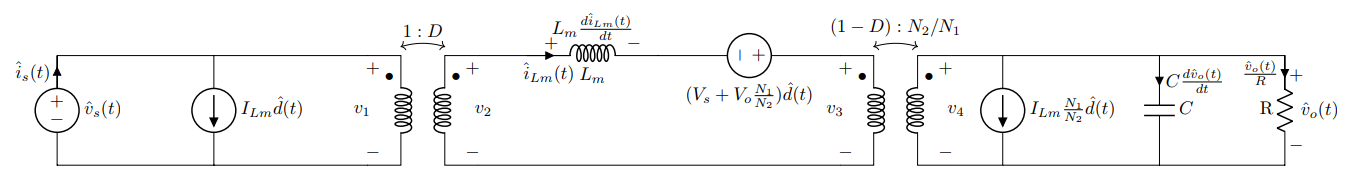
\includegraphics[width=1\textwidth]{Compensator/flyback_combined.png}
\caption{AC Small-Signal Equivalent Circuit of the Flyback Converter}
\label{com:fly_combined}
\end{center}
\end{figure}

This equivalent circuit can now be analyzed and solved by using the conventional linear circuit analysis techniques in order to obtain the necessary transfer functions.

\subsection{Transfer Function Derivation}

We analyze the derived small-signal ac equivalent circuit model of the Flyback Converter shown in Figure \ref{com:fly_combined} by using the conventional linear circuit analysis techniques in order to obtain the control to output transfer function of the Flyback Converter. The derived control to output transfer function then will be used in the compensator design stage in order to obtain the desired closed loop characteristics.

The control to output transfer function $G_{vd}(s)$ is found by setting the source (input) voltage variations $\hat{v}_s(s)$ to zero, and then solving the equivalent circuit model for the output voltage variations $\hat{v}_o(s)$ as a function of the control input variations $\hat{d}(s)$.

\begin{align}
   \left. G_{vd}(s) = \frac{\hat{v_o(s)}}{\hat{d}(s)}\right \vert_{\hat{v}_s(s) = 0}
\end{align}

As a result, we basically set the $\hat{v}_s(s)$ input voltage source to zero, and hence short circuit it. The resultant equivalent circuit is shown in Figure \ref{com:fly_tf1}, below.

\begin{figure}[H]
\begin{center}
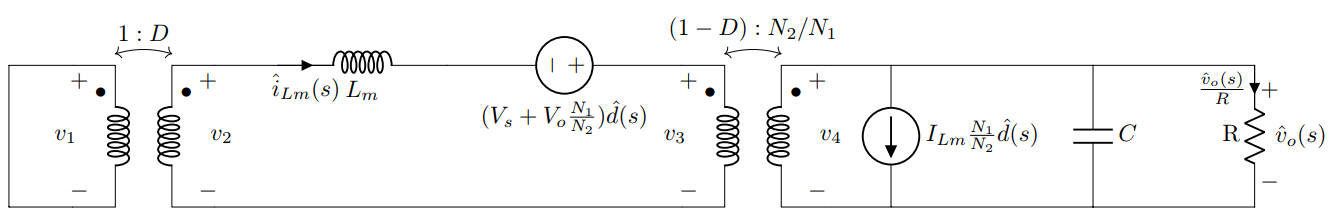
\includegraphics[width=1\textwidth]{Compensator/flyback_tf1.png}
\caption{Equivalent Circuit Model When $\hat{v}_s(s)$} Voltage Source is set to zero
\label{com:fly_tf1}
\end{center}
\end{figure}

Since the primary side of the first transformer is short circuited, its secondary side terminals are also short circuited. Then, we can simplify the above equivalent circuit as follows, as shown in Figure \ref{com:fly_tf1_1}, below.

\begin{figure}[H]
\begin{center}
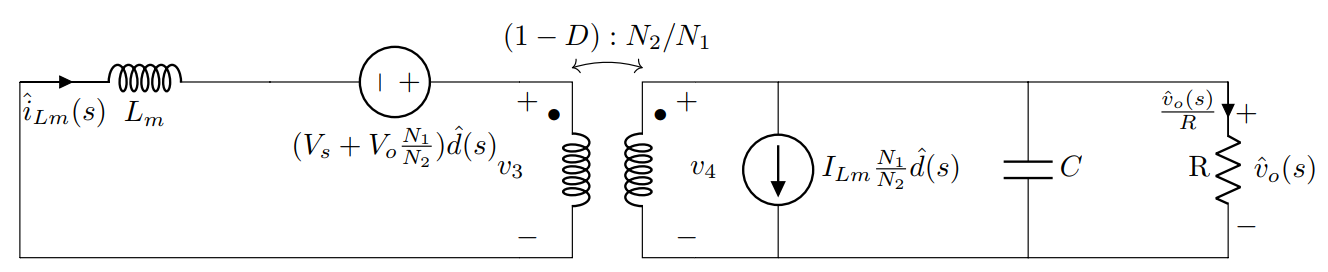
\includegraphics[width=1\textwidth]{Compensator/flyback_tf1_1.png}
\caption{Simplified Equivalent Circuit Model When $\hat{v}_s(s)$} Voltage Source is set to zero
\label{com:fly_tf1_1}
\end{center}
\end{figure}

This resultant equivalent circuit shown in Figure \ref{com:fly_tf1_1} two $\hat{d}$-dependent sources: one $\hat{d}$-dependent voltage source and one $\hat{d}$-dependent current source. Therefore, we need to use the principle of superposition in order to express the control to output transfer function. The control to output transfer function $G_{vd}(s)$ can be expressed as a superposition of terms arising from the independent effect of these two $\hat{d}$-dependent sources.

First of all, we set the $\hat{d}(s)$-dependent voltage source to zero, i.e. short circuited, and evaluate the effect of the $\hat{d}(s)$-dependent current source on the control to output transfer function.

The resultant equivalent circuit with the  $\hat{d}(s)$-dependent voltage source is set to zero is shown in Figure \ref{com:fly_tf2}, below.

\begin{figure}[H]
\begin{center}
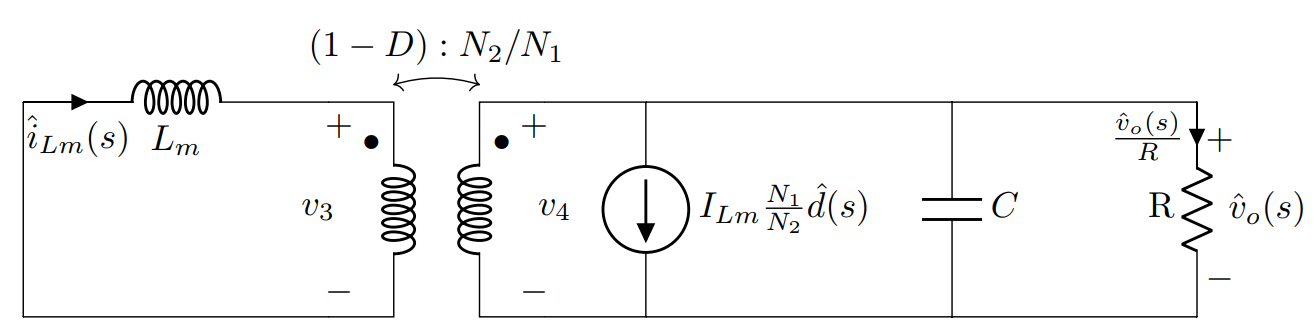
\includegraphics[width=1\textwidth]{Compensator/flyback_tf2.png}
\caption{Equivalent Circuit When $\hat{d}(s)$-dependent Voltage Source is set to zero}
\label{com:fly_tf2}
\end{center}
\end{figure}

The magnetizing inductor $L_m$ on the primary side of the transformer in Figure \ref{com:fly_tf2} can be pushed to the secondary side with the square of the turns ratio as shown in Figure \ref{com:fly_tf2_2}, below.

\begin{figure}[H]
\begin{center}
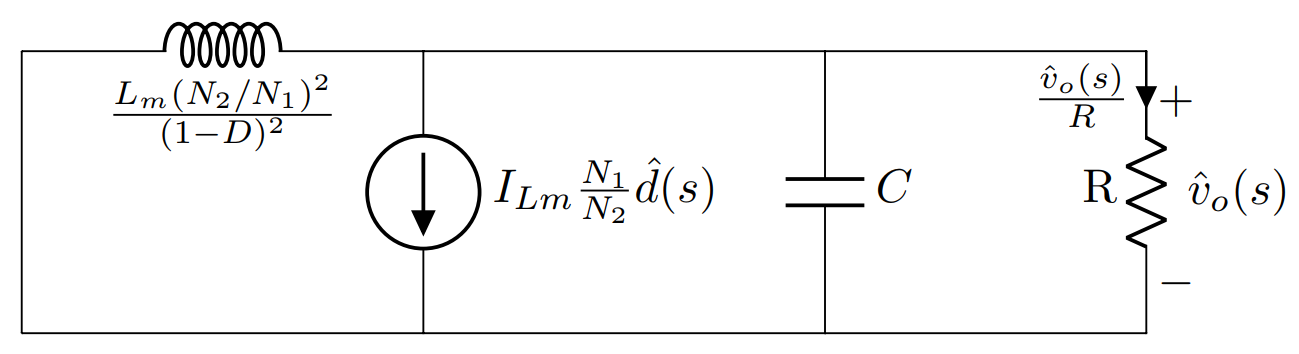
\includegraphics[width=1\textwidth]{Compensator/flyback_tf2_2.png}
\caption{Resultant Circuit When $\hat{d}(s)$-dependent Voltage Source is set to zero}
\label{com:fly_tf2_2}
\end{center}
\end{figure}

Then, we can solve this resultant circuit in order to obtain the first component of the control to output transfer ratio $\hat{v}_o(s)/\hat{d}(s)$ as follows.

We apply the KCL formulation to the resultant circuit.

From KCL:

\begin{align}
    \frac{\hat{v}_o(s)}{R} + \frac{\hat{v}_o(s)}{1/sC} + I_{Lm}\frac{N_1}{N_2}\hat{d}(s) + \frac{\hat{v}_o(s)}{s\frac{L_m(N_2/N_1)^2}{D'^2}} = 0
\end{align}

If we rearrange this equation, we obtain the following relation.

\begin{align}
    \hat{v}_o(s)\left[\frac{1}{R}+sC+\frac{D'^2}{sL_m(N_2/N_1)^2} \right] = -I_{Lm}\frac{N_1}{N_2}\hat{d}(s)
\end{align}

Finally, we obtain the first component of the control to output transfer function $G_{vd}(s)$ is obtained as follows.

\begin{align}
   \left. G_{vd1}(s) = \frac{\hat{v_o(s)}}{\hat{d}(s)}\right \vert_{\hat{v}_s(s) = 0} = \frac{-I_{Lm}(N_1/N_2)}{\frac{1}{R}+sC+\frac{D'^2}{sL_m(N_2/N_1)^2}}
\end{align}

\begin{align}
   \left. G_{vd1}(s) = \frac{\hat{v_o(s)}}{\hat{d}(s)}\right \vert_{\hat{v}_s(s) = 0} = -\frac{1}{D'^2}\frac{s[I_{Lm}L_m(N_2/N_1)]}{1+s\frac{L_m(N_2/N_1)^2}{RD'^2}+s^2\frac{L_mC(N_2/N_1)^2}{D'^2}}
\end{align}

Next, we set the $\hat{d}(s)$-dependent current source to zero, i.e. open circuited, and evaluate the effect of the $\hat{d}(s)$-dependent voltage source on the control to output transfer function.

The resultant equivalent circuit with the  $\hat{d}(s)$-dependent current source is set to zero, i.e. open circuited, is shown in Figure \ref{com:fly_tf3}, below.

\begin{figure}[H]
\begin{center}
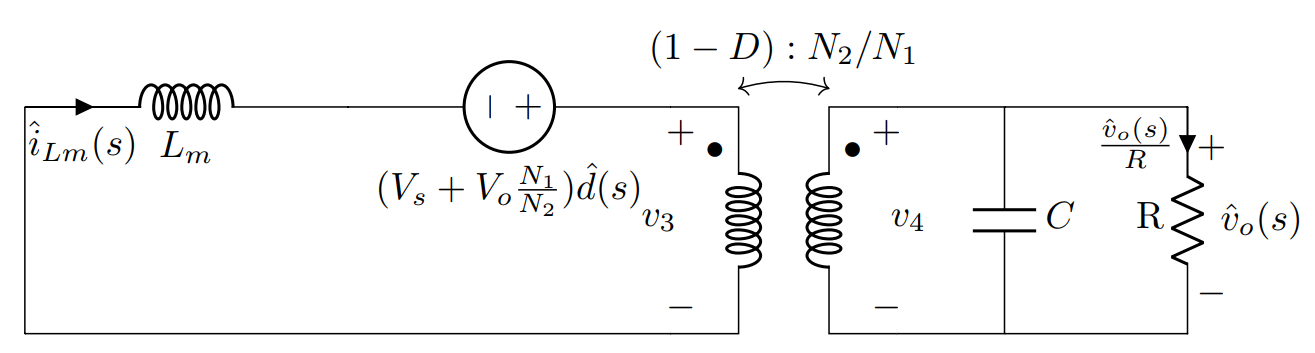
\includegraphics[width=1\textwidth]{Compensator/flyback_tf3.png}
\caption{Equivalent Circuit When $\hat{d}(s)$-dependent Current Source is set to zero}
\label{com:fly_tf3}
\end{center}
\end{figure}

In order to further simplify the resultant equivalent circuit for the transfer function analysis, the $\hat{d}(s)$-dependent voltage source and the magnetizing inductor $L_m$ on the primary side of the transformer in Figure \ref{com:fly_tf3} can be pushed to the secondary side of the transformer by using the turns ratio of the transformer as shown in Figure \ref{com:tf3}, below.

\begin{figure}[H]
\begin{center}
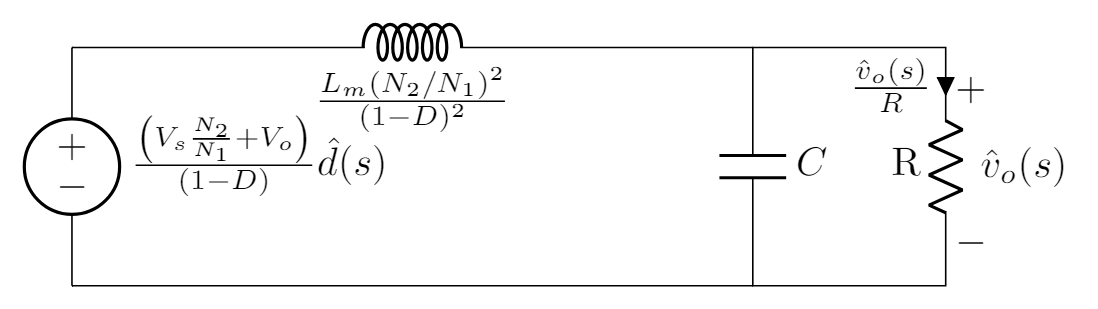
\includegraphics[width=1\textwidth]{Compensator/tf3.png}
\caption{Resultant Circuit When $\hat{d}(s)$-dependent Current Source is set to zero}
\label{com:tf3}
\end{center}
\end{figure}

Then, we can solve this resultant circuit in order to obtain the second component of the control to output transfer ratio $\hat{v}_o(s)/\hat{d}(s)$ as follows.

We apply the basic voltage division rule between the magnetizing inductor $L_m$ and the parallel output capacitor and load resistance.

\begin{align}
    \hat{v}_o(s) = \frac{\left(V_s\frac{N_2}{N_1}+V_o \right)}{D'}\hat{d}(s)\times\frac{R \parallel (1/sC)}{s\frac{L_m(N_2/N_1)^2}{D'^2} + \left(R \parallel (1/sC)\right)}
\end{align}

where

$$ R \parallel (1/sC) = \frac{R}{1+sRC} $$

Finally, we obtain the second component of the control to output transfer function $G_{vd}(s)$ is obtained as follows.

\begin{align}
   \left. G_{vd2}(s) = \frac{\hat{v_o(s)}}{\hat{d}(s)}\right \vert_{\hat{v}_s(s) = 0} = \left(V_s\frac{N_2}{N_1} + V_o \right)\frac{1}{D'}\frac{1}{R+s\frac{L_m(N_2/N_1)^2}{D'^2}+s^2\frac{RCL_m(N_2/N_1)^2}{D'^2}}
\end{align}

We also know from the steady-state analysis of the Flyback Converter circuit that its voltage transfer ratio is given as follows:

\begin{align}
    \frac{V_o}{V_s} = \frac{D}{1-D}\frac{N_2}{N_1}
\end{align}

Then, we can rewrite the $V_o$ in terms of $V_s$ as follows:

\begin{align}
    V_o = \frac{D}{1-D}\frac{N_2}{N_1}V_s
\end{align}

If we substitute this equality in the above equation, the following equivalence is obtained.

\begin{align}
    V_s\frac{N_2}{N_1}+V_o =  V_s\frac{N_2}{N_1} + \frac{D}{1-D}\frac{N_2}{N_1}V_s = \frac{V_s}{D'}\frac{N_2}{N_1}
\end{align}

We also divide both the numerator and the denominator of the above control to output transfer function by load resistance value R in order to put it in the most common form.

Then, the resultant second component of the control to output transfer function can be expressed as follows.

\begin{align}
   \left. G_{vd2}(s) = \frac{\hat{v_o(s)}}{\hat{d}(s)}\right \vert_{\hat{v}_s(s) = 0} = \left(\frac{V_s}{D'}\frac{N_2}{N_1}\right)\frac{1}{1 + s\frac{L_m(N_2/N_1)^2}{RD'^2} + s^2\frac{L_mC(N_2/N_1)^2}{D'^2}} 
\end{align}

Now, after obtaining the two components of the control to output transfer function $G_{vd}(s)$ separately, we can superpose them into the final expression for the control to output transfer function $G_{vd}(s)$ for the Flyback Converter by following the principle of superposition as follows:

\begin{align}
    G_{vd}(s) = G_{vd1}(s) + G_{vd2}(s)
\end{align}

Then, the control to output transfer function of the Flyback Converter is obtained as follows:

\begin{align}
   \left. G_{vd}(s) = \frac{\hat{v_o(s)}}{\hat{d}(s)}\right \vert_{\hat{v}_s(s) = 0} = \left[\frac{V_s}{D'}\frac{N_2}{N_1}-s\frac{I_{Lm}L_m}{D'^2}\frac{N_2}{N_1} \right]\frac{1}{1 + s\frac{L_m(N_2/N_1)^2}{RD'^2} + s^2\frac{L_mC(N_2/N_1)^2}{D'^2}}
\end{align}

We can rearrange it as follows:

\begin{align}
   \left. G_{vd}(s) = \frac{\hat{v_o(s)}}{\hat{d}(s)}\right \vert_{\hat{v}_s(s) = 0} = \left(\frac{1}{D'^2}\frac{N_2}{N_1} \right)\frac{V_s - sI_{Lm}L_m}{1 + s\frac{L_m(N_2/N_1)^2}{RD'^2} + s^2\frac{L_mC(N_2/N_1)^2}{D'^2}}
\end{align}

We can also rewrite the magnetizing inductance current $I_{Lm}$ as follows by starting from the steady-state expression for the magnetizing inductance current:

\begin{align}
    I_{Lm} = \frac{I_s}{D}
\end{align}

where the source (input) current $I_s$ can be found from the steady-state power relation as follows:

\begin{align}
    I_s = \frac{D}{1-D}\frac{N_2}{N_1}I_o =  \frac{D}{1-D}\frac{N_2}{N_1}\frac{V_o}{R}
\end{align}

We can also rewrite the output voltage $V_o$ in terms of the source (input) voltage $V_s$ as shown before.

$$ V_o = \frac{D}{1-D}\frac{N_2}{N_1}V_s $$

Then, the source (input) current $I_s$ is written as follows:

$$ I_s = \left(\frac{D}{1-D} \right)^2\left(\frac{N_2}{N_1} \right)^2\frac{V_s}{R} $$

Then, we can rewrite the magnetizing inductance current $I_{Lm}$ in terms of the source (input) voltage $V_s$ as follows by substituting the above source current equation into the magnetizing inductance current equation as shown below.

\begin{align}
    I_{Lm} =  \frac{D}{D'^2}\left(\frac{N_2}{N_1} \right)^2\frac{V_s}{R}
\end{align}

Finally, we can rearrange the control to output transfer function $G_{vd}(s)$ by substituting the above magnetizing inductance current $I_{Lm}$ relation into the computed control to output transfer function equation above.

\begin{align}
   \left. G_{vd}(s) = \frac{\hat{v_o(s)}}{\hat{d}(s)}\right \vert_{\hat{v}_s(s) = 0} = \left(\frac{V_s}{D'^2}\frac{N_2}{N_1} \right)\frac{1 - s\left[ \frac{D}{D'^2}\left(\frac{N_2}{N_1} \right)^2\frac{L_m}{R}\right]}{1 + s\frac{L_m(N_2/N_1)^2}{RD'^2} + s^2\frac{L_mC(N_2/N_1)^2}{D'^2}}
\end{align}

where $D' = 1-D$.

\begin{align}
   \left. G_{vd}(s) = \frac{\hat{v_o(s)}}{\hat{d}(s)}\right \vert_{\hat{v}_s(s) = 0} = \left(\frac{V_s}{(1-D)^2}\frac{N_2}{N_1} \right)\frac{1 - s\left[ \frac{D}{(1-D)^2}\left(\frac{N_2}{N_1} \right)^2\frac{L_m}{R}\right]}{1 + s\frac{L_m(N_2/N_1)^2}{R(1-D)^2} + s^2\frac{L_mC(N_2/N_1)^2}{(1-D)^2}}
\end{align}

\subsection{Compensator Design}

The control to output transfer function $G_{vd}(s)$ derived in the previous section is derived using the ideal Flyback Converter circuit. It is assumed that the output capacitor ESR and MOSFET on resistance are equal to zero. We used the ideal Flyback Converter circuit in the derivations of the small-signal ac equivalent circuit and the control to output transfer function of the converter topology in order to obtain the general form for the control to output transfer function. However, for the closed-loop control with the compensator design, we need to consider the non-idealities in the Flyback Converter circuit. Therefore, in this subsection, we will derive the control to output transfer function for the converter circuit including the non-idealities by using the derived control to output transfer function for the ideal Flyback Converter circuit in the previous part.

However, we will only include the output capacitor non-idealities, capacitor ESR, since it is specified in the project description that we may assume ideal switches for this stage. Therefore, the on resistance of the MOSFET switch is not included in the calculations of the control to output transfer function of the non-ideal Flyback Converter circuit. We will assume ideal switch characteristics with zero on resistance for this stage.

For that reason, we only need to include the non-idelities in the output capacitor. The output capacitor ESR must be taken into consideration.

We know from previous project works and EE464 lectures that the output capacitor ESR $R_c$ causes an addition of an extra zero in the control to output transfer function. The frequency of the additional zero due to output capacitor ESR is computed from the following relation.

\begin{align}
    \omega_{zESR} = \frac{1}{R_cC}
\end{align}

Then, the control to output transfer function $G_{vd}(s)$ for the non-ideal Flyback Converter circuit can be expressed in the following general form.

\begin{align}
   \left. G_{vd}(s) = \frac{\hat{v_o(s)}}{\hat{d}(s)}\right \vert_{\hat{v}_s(s) = 0} = G_{d0}\frac{\left(1+\frac{s}{\omega_{zERS}}\right)\left(1-\frac{s}{\omega_{zRHP}} \right)}{1+\frac{s}{\omega_0 Q}+\frac{s^2}{\omega_0^2}}
   \label{com:non_ideal_tf}
\end{align}

Where

\begin{align}
    G_{d0} = \frac{V_s}{D'^2}\left(\frac{N_2}{N_1} \right)
\end{align}

\begin{align}
    \omega_{zESR} = \frac{1}{R_cC}
\end{align}

\begin{align}
    \omega_{zRHP} = \frac{V_s}{I_{Lm}L_m} = \frac{D'^2}{D}\left(\frac{N_1}{N_2} \right)^2\frac{R}{L_m}
\end{align}

\begin{align}
    \omega_0 = \frac{D'}{\sqrt{L_mC}(N_2/N_1)}
\end{align}

\begin{align}
    Q = \frac{1}{\left[\frac{L_m(N_2/N_1)^2}{RD'^2} + R_cC \right]\omega_0}
\end{align}

As can be seen from equation \eqref{com:non_ideal_tf} above, the control to output transfer function includes two zeros and two poles. One of the zeros $\omega_{zESR}$ is due to the output capacitor ESR as mentioned before. This zero is on the LHP of the complex plane, and hence it is a stable zero. The other zero of the transfer function $\omega_{zRHP}$ is actually the most critical one because it is an unstable zero with positive real part. This zero is located on the RHP of the complex plane as its name suggests. Therefore, it has a positive real part, and hence an unstable zero. This RHP zero makes the control of the converter circuit very difficult. Furthermore, the control to output transfer function has double pole at the resonant frequency $\omega_0$ due to the LC filter.

After obtaining the expressions for the control to output transfer functions for the ideal and the non-ideal Flyback Converter circuit, we can compare and investigate their bode plots.

The following figures shows the comparison of the bode plots for the ideal and non-ideal Flyback Converter with their respective critical stability margins and peak gains.

\begin{figure}[H]
\begin{center}
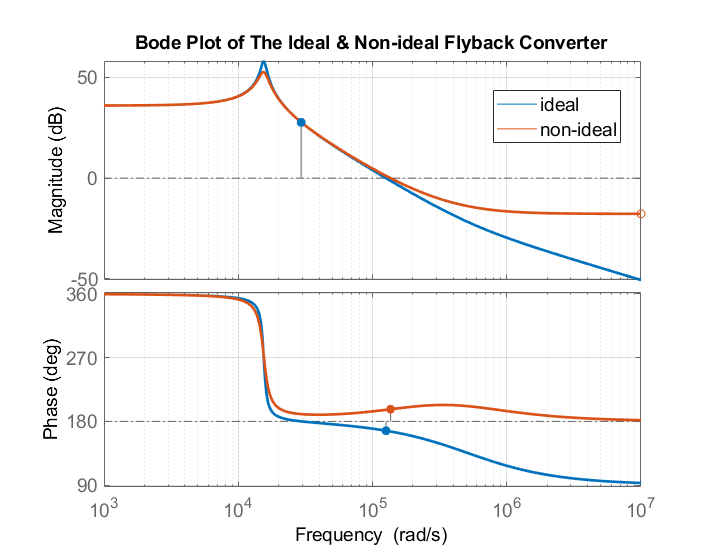
\includegraphics[width=0.8\textwidth]{bode_plots/bode2.png}
\caption{Bode Plots of the Ideal and Non-ideal Flyback Converter}
\label{com:bode2}
\end{center}
\end{figure}

\begin{figure}[H]
\begin{center}
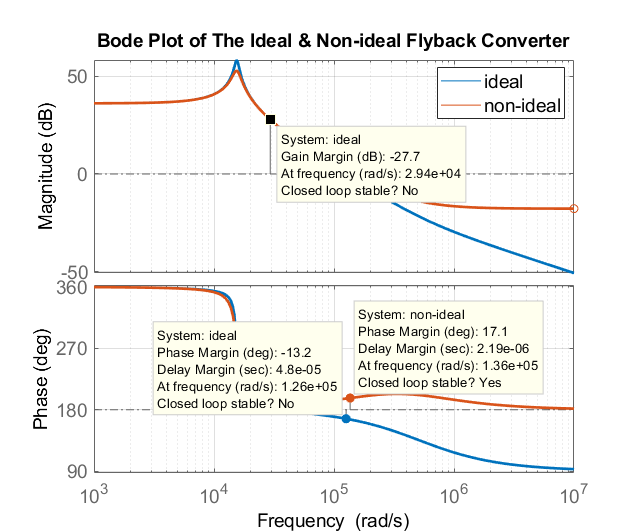
\includegraphics[width=0.8\textwidth]{bode_plots/gain_margin.png}
\caption{Stability Margins of the Ideal and Non-ideal Flyback Converter}
\label{com:bode3}
\end{center}
\end{figure}

It is observed from Figure \ref{com:bode3} that there is a huge deviation between the gain and phase plots of the ideal and the non-ideal Flyback Converter bode plots at high frequencies. This deviation occurs as a result of the additional zero in the non-ideal Flyback Converter transfer function due to the output capacitor ESR. The additional ESR zero lifts the phase and the gain curves of the non-ideal Flyback Converter bode plot up at high frequencies compared to the ideal case, and in a way provides phase boost.

It is shown in Figure \ref{com:bode3} that the ideal Flyback Converter has a phase margin of -13.2 degrees.

$$ \phi_m = -13.2\degree $$

This result shows that the uncompensated ideal Flyback Converter is unstable since its phase margin is negative ($ \phi_m = -13.2\degree < 0 $).

The ideal Flyback Converter has also a gain margin of -27.7 dB as shown in Figure \ref{com:bode3}.

$$ G_{dB} = -27.7 dB $$

Next, we look at the phase margin of the non-ideal Flyback Converter. It is observed from Figure \ref{com:bode3} that the non-ideal Flyback Converter has a phase margin of +17.1 degrees.

$$ \phi_m = 17.1\degree $$

Hence, we can see that the uncompensated non-ideal Flyback Converter is stable with a phase margin of 17.1 degrees since its phase margin is positive ($ \phi_m = 17.1\degree > 0 $).

As a result, it is concluded that the non-idealities in the converter circuit even causes stability change in the uncompensated open loop Flyback Converter circuit. This result is actually somehow expected since as explained before, the additional zero due to output capacitor ESR in the non-ideal Flyback Converter lifts up the phase plot and provides phase boost at high frequencies, which, in result, increases the phase margin.

The stability of the uncompensated non-ideal Flyback Converter circuit will facilitate the compensator design work since we will try to increase the phase margin of an already stable system. This will require less effort compared to the compensator design work for the ideal Flyback Converter circuit, in which case greater phase boost by the designed compensator is required due to the unstable open loop characteristics of the ideal Flyback Converter circuit.

\begin{figure}[H]
\begin{center}
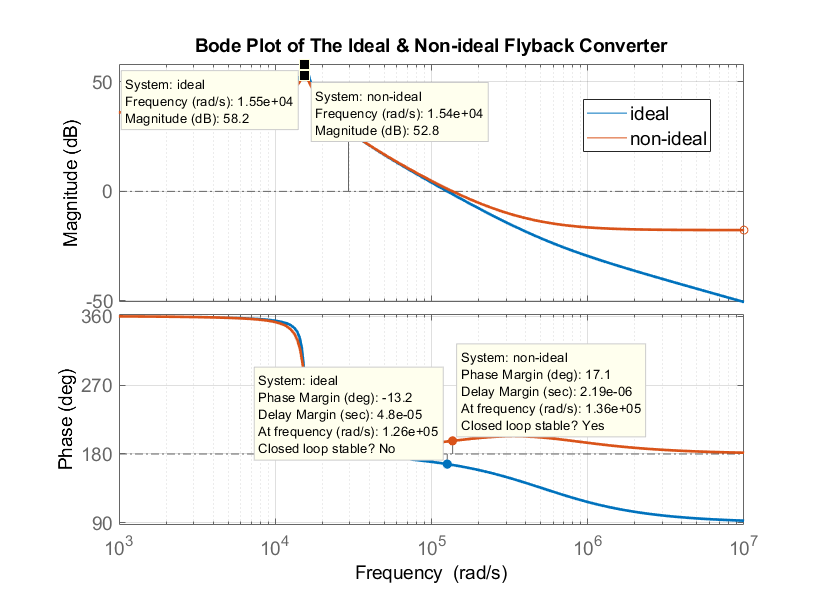
\includegraphics[width=0.8\textwidth]{bode_plots/bode4.png}
\caption{Peak Gains of the Ideal and Non-ideal Flyback Converter}
\label{com:bode4}
\end{center}
\end{figure}

In Figure \ref{com:bode4}, we observe the peak gains of the ideal and the non-ideal Flyback Converter circuits. It is shown that the ideal Flyback Converter circuit has a peak gain of 58.2 dB while the non-ideal Flyback Converter circuit has a peak gain of 52.8 dB.

The peak gain occurs at the resonant frequency $\omega_0$ due to the LC resonant. The resonant in the LC circuit might cause huge gain peaks in the magnitude plot. These peak gains are actually quite undesirable since they can cause undesirable faulty operation of the converter circuit. Therefore, it is desired to keep this peak gain in the converter magnitude plot as small as possible.

It is seen that the non-ideal Flyback Converter has smaller peak gain (52.8 dB) than the ideal Flyback Converter (58.2 dB), as given above. As a result, we might conclude that the non-ideal Flyback Converter has more desirable characteristics compared to the ideal Flyback Converter also in terms of peak gain performance.

\begin{figure}[H]
\begin{center}
\includegraphics[width=0.8\textwidth]{bode_plots/bode5.png}
\caption{Bode Plot of the Non-ideal Flyback Converter}
\label{com:bode5}
\end{center}
\end{figure}

\begin{figure}[H]
\begin{center}
\includegraphics[width=0.8\textwidth]{bode_plots/bode7.png}
\caption{Stability Margins and the Peak Gain of the Non-ideal Flyback Converter}
\label{com:bode7}
\end{center}
\end{figure}

Now, we need to compute the pole and zero frequencies of the non-ideal Flyback Converter with the selected component parameters in order to decide on the compensator type to be designed and calculate the circuit component parameters for the selected compensator type.

First of all, let us rewrite the non-ideal Flyback Converter circuit component parameters and input to output current, voltage and power specifications as follows:

\begin{table}[H]
    \centering
    \caption{Flyback Converter Circuit Component Parameters \& Specifications}
    \begin{tabular}{|c|c|c|c|c|c|}
    \hline
\textbf{Paremeter}   & \textbf{Value}          & \textbf{Parameter}      & \textbf{Value}          & \textbf{Parameter} & \textbf{Value}         \\ \hline
L_m & 28.67 \micro H & C & 220 \micro F & R_c & 20 m\ohm \\ \hline
$V_{out}$ & 15 V & $I_{out}$ & 4 A & $P_{out}$ & 60 W \\ \hline
$V_{in}$ & 48 V & $N_1$ & 10 turns & $N_2$ & 5 turns \\ \hline
R & 3.75 \ohm & $I_{in}$ & 1.25 A & - & - \\ \hline
    \end{tabular}
    \label{tab:spec_com}
\end{table}

Now, we can finally compute the pole and zero frequencies of the non-ideal Flyback Converter by substituting the circuit parameter values given in Table \ref{tab:spec_com} to the pole zero frequency equations given above.

The Table \ref{} below shows the computed pole and zero frequencies for the non-ideal Flyback Converter in rad/s.

\begin{table}[H]
    \centering
    \caption{Pole \& Zero Frequencies}
    \begin{tabular}{|c|c|}
    \hline
\textbf{Paremeter}   & \textbf{Value}        \\ \hline
$\omega_{zESR}$ & 2.2727\times 10^5\; rad/s   \\ \hline
$\omega_{zRHP}$ & 5.1515\times 10^5\; rad/s   \\ \hline
$\omega_{LC}$ &  1.5797\times 10^4\; rad/s   \\ \hline
    \end{tabular}
    \label{tab:freq_rad}
\end{table}

The corresponding pole and zero frequencies can be written in terms of hertz as follows:

\begin{table}[H]
    \centering
    \caption{Pole \& Zero Frequencies}
    \begin{tabular}{|c|c|}
    \hline
\textbf{Paremeter}   & \textbf{Value}        \\ \hline
$f_{zESR}$ & 36.172 kHz   \\ \hline
$f_{zRHP}$ & 81.988 kHz   \\ \hline
$f_{LC}$ & 2.4664 kHz   \\ \hline
    \end{tabular}
    \label{tab:freq_rad}
\end{table}

We also have a switching frequency $f_s$ of 45 kHz.

$$ f_s = 45\; kHz $$

In many application notes on compensator design for DC/DC converters, it is stated that the crossover frequency $f_0$ should be less than or equal to about one-tenth of the switching frequency $f_s$.

Therefore, the crossover frequency should satisfy the following condition.

$$ f_0 < f_s/10 $$

Then, for our project we need the crossover frequency to be less than 4.5 kHz.

$$ f_0 < 4.5\; kHz $$

As a result, we decided to select the crossover frequency of 4 kHz.

$$ f_0 = 4\; kHz $$

We decided to choose maximum achievable crossover frequency $f_0$ since the higher crossover frequency increases the system response speed and bandwidth of the system.

Now, we need to decide on a compensator type to used in the compensator design according to the computed pole \& zero frequencies, crossover frequency and the switching frequency.

The following table taken from an application note shows the general rule for selecting the appropriate compensator type for the given DC/DC converter design application depending on the location of the pole \& zero frequencies of the converter circuit, selected crossover frequency and the switching frequency.

\begin{figure}[H]
\begin{center}
\includegraphics[width=0.8\textwidth]{Compensator/comp_type.png}
\caption{The compensation type and location of pole \& zero, crossover and switching frequency}
\label{com:comp_type}
\end{center}
\end{figure}

In our project, we have the following relation between the  pole \& zero frequencies of the converter circuit, selected crossover frequency and the switching frequency.

\begin{align}
    f_{LC} < f_{0} < \frac{f_s}{2} < f_{zESR}
\end{align}

$$ 2.4664\; kHz < 4\; kHz < 22.5\; kHz < 36.172\; kHz $$

As a result, according to the given table, we need to design a Type III B (PID) compensator for the non-ideal Flyback Converter circuit in our project.

The circuit schematic of the Type III compensator is shown in Figure \ref{com:type3b}, below.

\begin{figure}[H]
\begin{center}
\includegraphics[width=0.8\textwidth]{Compensator/type3b.png}
\caption{Circuit Schematic of the Type III Compensator}
\label{com:type3b}
\end{center}
\end{figure}

For the parameter calculations of the Type III B compensator, whose circuit schematic is given in Figure \ref{com:type3b}, below, I followed the design guidelines provided in the application note of Infineon: Compensator Design Procedure for Buck Converter with Voltage-Mode Error-Amplifier.

The transfer function of the Type III compensator is given as follows:

\begin{align}
    H(s) = \frac{V_e}{V_{out}} = \frac{Z_c}{Z_f}
\end{align}

\begin{align}
    H(s) = \frac{(1+sR_{C1}C_{C1})[1+sC_{f3}(R_{f1}+R_{f3})]}{sR_{f1}(C_{C1}+C_{C2})\left[1 + sR_{C1}\left(\frac{C_{C1}C_{C2}}{C_{C1}+C_{C2}} \right) \right](1+sR_{f3}C_{f3})}
\end{align}

The pole which is generated by $C_{C2}$ and $R_{C1}$ is usually set at a much higher frequency as compared with the frequency of the zero generated by $C_{C1}$ and $R_{C1}$ . This means: $C_{C2} << C_{C1}$. Therefore, it can be approximated as:

\begin{align}
    H(s) \approx \frac{(1+sR_{C1}C_{C1})[1+sC_{f3}(R_{f1}+R_{f3})]}{sR_{f1}C_{C1}(1 + sR_{C1}C_{C2})(1+sR_{f3}C_{f3})}
\end{align}

Then, the pole and zero frequencies of the compensator is found as follows:

The Type III compensator has two zeros and three poles:

\begin{align}
    F_{z1} = \frac{1}{2\pi R_{C1}C_{C1}}
\end{align}

\begin{align}
    F_{z2} = \frac{1}{2\pi C_{f3}(R_{f1}+R_{f3})}
\end{align}

\begin{align}
    F_{p1} = 0
\end{align}

\begin{align}
    F_{p2} = \frac{1}{2\pi R_{f3}C_{f3}}
\end{align}

\begin{align}
    F_{p3} = \frac{1}{2\pi R_{C1}C_{C2}}
\end{align}

Now, we have to decide on the compensator pole and zero locations depending on the non-ideal Flyback Converter pole \& zero locations, crossover frequency and the switching frequency.

The design procedure for selecting the pole and zero locations of the compensator for the Type III B compensator is given as follows:

\begin{itemize}
    \item The first pole of the compensator is placed at the origin to form an integrator.
    \item The compensator zeros are placed around the power stage resonant frequency.
    \item The second pole of the compensator is placed coincident with the ESR zero frequency of the power stage.
    \item The third pole of the compensator is placed coincident with the RHP zero frequency of the power stage.
    \item If the frequency of the RHP zero or ESR zero is higher than half the switching frequency, the corresponding compensation pole is placed at half the switching frequency.
\end{itemize}

According to these design tips, the compensator zero frequencies are chosen as the power stage resonant frequency of the non-ideal Flyback Converter.

$$ F_{z1} = f_{LC} = 2.4664\;kHz $$

$$ F_{z2} = f_{LC} = 2.4664\;kHz $$

The second pole of the compensator is placed at the half of the switching frequency since the ESR zero frequency of the power stage of the non-ideal Flyback Converter is higher than the switching frequency.

$$ F_{p2} = \frac{f_s}{2} = 22.5\;kHz $$

The third pole of the compensator is placed coincident with the RHP zero frequency of the power stage of the non-ideal Flyback Converter.

$$ F_{p3} = f_{zRHP} = 81.988\;kHz $$

Now, after selecting the compensator pole and zero frequencies, we can determine the circuit parameter values (resistor and capacitor values) for the Type III compensator.

First of all, we need to select a capacitance value for the capacitor $C_{f3}$. A few nano farad values are appropriate. After a number of trials, we decided to choose 10 nF for the capacitor $C_{f3}$.

$$ C_{f3} = 10\; nF $$

After determining $C_{f3}$, we can calculate $R_{f3}$ from following relation.

\begin{align}
    R_{f3} = \frac{1}{2\pi C_{f3}F_{p2}}
\end{align}

It is computed as:

$$ R_{f3} = 194.1198\;\ohm $$

Next, we determine $R_{f1}$ from $R_{f3}$ and $C_{f3}$ as follows:

\begin{align}
    R_{f1} = \frac{1}{2\pi C_{f3}F_{z2}} - R_{f3}
\end{align}

It is computed as:

$$ R_{f1} = 6.2587\;k\ohm $$

Next, we determine $R_{f2}$ from the voltage division rule between $V_{ref}$ and $V_{out}$ as follows:

\begin{align}
    R_{f2} = \frac{V_{ref}}{(V_{out}-V_{ref})}R_{f1}
\end{align}

In our project design, we selected the reference voltage value $V_{ref}$ as 1.2V.

\begin{align}
    V_{ref} = 1.2\;V
\end{align}

Then, $R_{f2}$ is computed as:

$$ R_{f2} = 544.2335\;\ohm $$

Next, we compute $R_{C1}$. There are several formulas and methods for computing this resistance value given in the application notes. However, none of them worked out properly for our design. Therefore, we decided to implement it by hand. After several trials, we have seen that $R_{C1}$ resistance value of 1 k\ohm provides very satisfactory results in terms of phase margin and closed loop behavior as well as ensuring reasonable parameter values for the capacitors $C_{C1}$ and $C_{C2}$.

It is selected as:

$$ R_{C1} = 1\;k\ohm $$

Then, we can determine the capacitance values for the capacitors $C_{C1}$ and $C_{C2}$ by using the selected $ R_{C1}$ value according to the following relations.

\begin{align}
    C_{C1} = \frac{1}{2\pi R_{C1}F_{z1}}
\end{align}

\begin{align}
    C_{C2} = \frac{1}{2\pi R_{C1}F_{p3}}
\end{align}

Then, the capacitance $C_{C1}$ is computed as:

$$ C_{C1} = 64.528\;nF $$

The capacitance $C_{C2}$ is computed as:

$$ C_{C2} = 7.0736\;nF $$

Now, parameter calculation part is completed. However, we cannot use these values for the compensator circuit components since these values are not available as a commercial product. Therefore, we need to round up or down these parameter values to the closest available commercial product values.

After the rounding operation, the final values of the compensator circuit elements are obtained as given in the Table \ref{tab:comp_para}, below.

\begin{table}[H]
    \centering
    \caption{Rounded Compensator Circuit Parameter Values}
    \begin{tabular}{|c|c|c|c|}
    \hline
\textbf{Paremeter}   & \textbf{Value} 
& \textbf{Paremeter}   & \textbf{Value} \\ \hline
$R_{f1}$ & 6.2 k\ohm & $R_{f2}$ &  540 \ohm \\ \hline
$R_{f3}$ & 200 \ohm & $R_{C1}$ & 1 k\ohm \\ \hline
$C_{C1}$ & 65 nF & $C_{C2}$ & 7 nF \\ \hline
$C_{f3}$ & 10 nF & - & - \\ \hline
    \end{tabular}
    \label{tab:comp_para}
\end{table}

After attaining the compensator parameter values, we can construct the closed loop block diagram of the overall compensated Flyback Converter system as shown in Figure \ref{com:CL_block}, below.

\begin{figure}[H]
\begin{center}
\includegraphics[width=0.8\textwidth]{Compensator/CL_block_diagram.png}
\caption{Closed Loop Block Diagram of the Compensated Flyback Converter}
\label{com:CL_block}
\end{center}
\end{figure}

Here, the transfer function block $G_p(s)$ represents the power stage control to output transfer function of the non-ideal Flyback Converter. Then, the overall transfer function $G(s)$, as shown in the figure, is obtained by combining the transfer functions of the power stage $G_p(s)$ and the PWM Generator $\left(\frac{1}{V_{osc}} \right)$ as follows:

\begin{align}
    G(s) = G_p(s)\frac{1}{V_{osc}}
\end{align}

The PWM Generator has simply a gain of $1/V_{osc}$ where $V_{osc}$ is the peak to peak amplitude of the oscillator voltage (saw-tooth) which is used in the comparator circuit for the comparison with the reference signal in order to generate the necessary PWM signals with adjusted duty ratio to drive the MOSFET switch of the Flyback Converter.

In our project design, we selected the peak to peak amplitude of the oscillator voltage (saw-tooth) $V_{osc}$ as 1.8V in order to limit the maximum duty cycle of the switch to 66.67\%

As we know, the maximum duty ratio is limited by the peak amplitudes of the carrier (control) signal, which is the oscillator saw-tooth waveform, and the reference signal.

In our project, we have selected reference signal voltage level as 1.2V and peak to peak amplitude of the oscillator voltage (saw-tooth) as 1.8V. Then, the maximum achievable duty ratio is computed as follows:

\begin{align}
    D_{max} = \frac{V_{ref}}{V_{osc}} = \frac{1.2}{1.8} = 0.6667\;(or\; 66.67\%)
\end{align}

Then, the open loop gain of the constructed closed loop system is obtained as follows:

\begin{align}
    M(s) = \frac{1}{k}\times H(s)\times G_p(s)\frac{1}{V_{osc}} = \frac{1}{k}\times H(s)\times G(s)
\end{align}

where 1/k represents the gain of the resistor divider which is used in the feedback loop when  $V_{out} > V_{ref}$. For the configuration given in this design method, this term is cancelled out, and does not appear in the loop gain transfer function.

As a result, the open loop gain transfer function is rewritten as follows:

\begin{align}
    M(s) = H(s)\times G_p(s)\frac{1}{V_{osc}} = H(s)\times G(s)
\end{align}

Now, finally, we can construct the relevant bode plots for the designed compensator and the open loop system.

The following figure shows the bode plots of the power stage $G_p(s)$ and the combined transfer function $G(s)$ on the same figure.

\begin{figure}[H]
\begin{center}
\includegraphics[width=0.8\textwidth]{bode_plots/G_Gp_bode1.png}
\caption{Bode Plots of the Power Stage $G_p(s)$ and the Combined Transfer Function $G(s)$}
\label{com:G_Gp_bode1}
\end{center}
\end{figure}

The Figure \ref{com:G_Gp_bode2} shows the critical stability margins for the both transfer functions.

\begin{figure}[H]
\begin{center}
\includegraphics[width=0.8\textwidth]{bode_plots/G_Gp_bode2.png}
\caption{Stability Margins of the Power Stage $G_p(s)$ and the Combined Transfer Function $G(s)$}
\label{com:G_Gp_bode2}
\end{center}
\end{figure}

As can be seen from Figure \ref{com:G_Gp_bode1}, both transfer functions have the same phase plot. However, the magnitude plot of the combined transfer function $G(s)$ is shifted down with respect to the power stage transfer function $G_p(s)$. This, in result, causes the phase margin and the gain crossover frequency of the combined transfer function to decrease compared to the power stage transfer function. Hence, the combined transfer function has smaller bandwidth with smaller stablity margin. This result is actually expected since the PWM Generator gain $1/V_{osc}$ is smaller than one (1/1.8 = 0.55), which shifts the magnitude plot down. However, the proportional gain does not affect the phase plot. Hence, the phase plot are the same for both transfer functions. This results in decrease in the phase margin and the bandwidth.

The bode plot of the designed Type III B compensator circuit is shown in Figure \ref{com:comp_bode}, below.

\begin{figure}[H]
\begin{center}
\includegraphics[width=0.8\textwidth]{bode_plots/comp_bode.png}
\caption{Bode Plot of the Designed Type III B Compensator}
\label{com:comp_bode}
\end{center}
\end{figure}

The bode plot of the open loop compensated system is shown in Figure \ref{com:openloop_bode1}, below.

\begin{figure}[H]
\begin{center}
\includegraphics[width=0.8\textwidth]{bode_plots/OpenLoop_bode1.png}
\caption{Bode Plot of the Open Loop Compensated System}
\label{com:openloop_bode1}
\end{center}
\end{figure}

The critical stability margins of the open loop compensated system is shown in Figure \ref{com:openloop_bode2}, below.

\begin{figure}[H]
\begin{center}
\includegraphics[width=0.8\textwidth]{bode_plots/OpenLoop_bode2.png}
\caption{Stability Margins of the Open Loop Compensated System}
\label{com:openloop_bode2}
\end{center}
\end{figure}

It is seen from Figure \ref{com:openloop_bode2} that the open loop compensated system has a gain margin of 17 dB at 412 krad/s.

\begin{align}
    G_{dB} = 17\;dB \;(@\;\omega = 412\;krad/s)
\end{align}

It is also observed that the open loop compensated system has a phase margin of 44.4 degrees at 80.2 krad/s as shown in the figure.

\begin{align}
    \phi_{m} = 44.4\degree \;(@\;\omega = 80.2\;krad/s)
\end{align}

As a result, we can clearly observe that the closed loop system is stable, which is the desired outcome. The positive phase margin indicates that the closed loop system is stable. Our purpose for designing a compensator for the non-ideal Flyback Converter was to increase the stability of the system by increasing its phase margin, and operate it in the stable region with a reasonable phase margin and response speed. The phase margin of 44.4 degrees is a quite satisfactory value for the stable closed loop operation of the converter circuit with enough damping (limited overshoot \& oscillations). The phase margin of 44.4 degrees ensures that the system will be able to operate in the stable region, and preserve its stability for any kind of load changes and variations in the source (input) voltage or duty cycle.

The phase margin of the uncompensated non-ideal Flyback Converter was equal to 17.1 degrees. The phase margin of the compensated Flyback Converter system is increased to 44.4 degrees with the design of a Type III B compensator. As a result, the designed compensator provided a phase boost of around 27.3 degrees by boosting the phase margin of the non-ideal converter system from 17.1 degrees to 44.4 degrees.

The peak gain and the gain crossover frequency data points of the open loop compensated system is indicated on the bode plot in the following figure.

\begin{figure}[H]
\begin{center}
\includegraphics[width=0.8\textwidth]{bode_plots/OpenLoop_bode3.png}
\caption{Peak Gain \& Gain Crossover Frequency of the Open Loop Compensated System}
\label{com:openloop_bode3}
\end{center}
\end{figure}

Another important parameter for the closed loop performance of the designed converter system is the gain crossover frequency or the bandwidth of the open loop compensated system. The bandwidth or the gain crossover frequency of a system determines the response speed of the system to the reference signal or disturbance signal changes. The larger bandwidth or gain crossover frequency means that the system has a fast response with smaller settling time. In other words, the response speed of the system to the reference or disturbance signal changes increases with the increasing bandwidth or gain crossover frequency. Therefore, it is our desire to achieve a high enough bandwidth value as well as a high phase margin in order to ensure that the system has a good response speed.

The gain crossover frequency is defined as the frequency at which the magnitude plot of the open loop compensated system crosses the zero dB (0 dB) line, which corresponds to unity gain ($Gain = |G(s)H(s)| = 1$). In other words, the crossover frequency is the frequency at which the magnitude of the loop gain is unity.

It is observed from Figure \ref{com:openloop_bode3} that the open loop compensated system has a gain crossover frequency of around 80 krad/s.

\begin{align}
    \omega_G = 80\;krad/s
\end{align}

The gain crossover frequency of the open loop system G(s)H(s) is regarded approximately equal to the bandwidth of the system, which is measured from the unit gain crossing point in the magnitude bode plot of the complementary sensitivity transfer function.

\begin{align}
    \omega_G \approx \omega_B = 80\;krad/s
\end{align}

This result indicates that the closed loop system will have a reasonably fast response to the reference signal changes.

One final remark is on the peak gain in the magnitude plot of the open loop compensated system. As mentioned before, this peak gain in the non-ideal Flyback Converter magnitude plot occurs at the resonant frequency due to the LC resonant in the converter circuit. We also stated that this peak in the gain is quite undesirable for the proper circuit operation, and hence we want to minimize it as much as possible. 

The Figure \ref{com:openloop_bode3} shows that the peak gain in the LC resonant frequency is equal to 36.8 dB, which is not very high in comparison with the linearly decreasing curve around the resonant frequency. This result shows that we were able to repress the peak gain around the resonant frequency reasonably enough by keeping it as small as possible so that it cannot significantly affect the stable converter circuit operation.

\subsection{Simulations of the Closed Loop Control System}

In this subsection of the report, we will provide the simulation results of the designed closed loop system to variations in the output load and the source (input) voltage in order to investigate the response of the converter circuit to these changes, and see whether the closed loop system is able to achieve the required performance metrics that defined in the previous subsection. We will observe if the closed loop behaviour of the circuit complies with the measured performance and stability metrics in the previous part.

We will use the LTSpice simulation software to make our simulations.

\subsubsection{Load Change from Full Load to Half Load}

First of all, we will simulate the load change condition from full load to half load at the source (input) voltage of 48V.

The LTSpice circuit schematic of the compensated non-ideal Flyback Converter circuit is given in Figure \ref{com:schematic_FH} below for the load switch from full load to half load.

\begin{figure}[H]
\begin{center}
\includegraphics[width=1\textwidth]{comp_simulations/schematic_FH.png}
\caption{LTSpice Circuit Schematic of the Compensated Non-ideal Flyback Converter}
\label{com:schematic_FH}
\end{center}
\end{figure}

The circuit schematic is modified in order to simulate the load switching condition from full load to half load. Two parallel load resistances with the resistance value of the double of the full load resistance value (3.75 \ohm) are connected at the load side of the converter. One of the parallel resistances is activated or deactivated by using a MOSFET switch in series with the relevant resistance on the same branch. This semiconductor switch (M2 in the figure) is basically used to control the load change operation from the full load to half load condition.

In the full load operation, the output load resistance should be equal to the full load resistance, which is 3.75 \ohm. Therefore, the load side switch (M2 in the figure) must be kept on during this period. Then, the load resistance must be switched to 7.5 \ohm in order to switch the load to half load condition. For the half load condition, the load resistance should be doubled in order to reduce the load current. Therefore, the load side switch M2 must be turned off during the second half period of the simulation in order to keep the load resistance at 7.5 \ohm.

The gate signal that needs to be generated to drive the load side switch M2, therefore, is given as follows in Figure \ref{com:pulse_FH}.

\begin{figure}[H]
\begin{center}
\includegraphics[width=1\textwidth]{comp_simulations/pulse_FH.png}
\caption{Gate Driver Pulse Signal of the Load Side Switch M2}
\label{com:pulse_FH}
\end{center}
\end{figure}

As can be seen from Figure \ref{com:pulse_FH}, the load is switched from full load to half load at time t = 5 ms since the load side switch M2 is activated with a gate signal of 5V during the first 5 ms period of the simulation, and then the gate signal is switched to 0V for the second 5 ms period of the simulation meaning that the load side switch M2 is deactivated.

The output voltage waveform of the compensated non-ideal Flyback Converter for the load switch from full load to half load is shown in Figure \ref{com:Vout_FH}, below.

\begin{figure}[H]
\begin{center}
\includegraphics[width=1\textwidth]{comp_simulations/Vout_FH.png}
\caption{Output Voltage Waveform for Load Switch From Full Load to Half Load}
\label{com:Vout_FH}
\end{center}
\end{figure}

The output load current waveform of the compensated non-ideal Flyback Converter for the load switch from full load to half load is shown in Figure \ref{com:Iload_FH}, below.

\begin{figure}[H]
\begin{center}
\includegraphics[width=1\textwidth]{comp_simulations/Iload_FH.png}
\caption{Output Load Current Waveform for Load Switch From Full Load to Half Load}
\label{com:Iload_FH}
\end{center}
\end{figure}

The magnetizing inductor current waveform of the compensated non-ideal Flyback Converter for the load switch from full load to half load is shown in Figure \ref{com:ILm_FH}, below.

\begin{figure}[H]
\begin{center}
\includegraphics[width=1\textwidth]{comp_simulations/ILm_FH.png}
\caption{Magnetizing Inductor Current Waveform for Load Switch From Full Load to Half Load}
\label{com:ILm_FH}
\end{center}
\end{figure}

In order to observe the duty ratio change from full load to half load condition, we will investigate the output voltage waveform $V_{error}$ of the error amplifier in the compensator circuit.

The error amplifier output voltage waveform of the compensator circuit for the load switch from full load to half load is shown in Figure \ref{com:Verror_FH}, below.

\begin{figure}[H]
\begin{center}
\includegraphics[width=1\textwidth]{comp_simulations/Verror_FH.png}
\caption{Error Amplifier Output Voltage Waveform for Load Switch From Full Load to Half Load}
\label{com:Verror_FH}
\end{center}
\end{figure}

We can also look at the zoomed view of the PWM gate signal of the Flyback Converter switch M1 around the load switching time of 5 ms.

The PWM gate signal waveform of the Flyback Converter switch M1 for the load switch from full load to half load is shown in Figure \ref{com:dutycycle_FH}, below.

\begin{figure}[H]
\begin{center}
\includegraphics[width=1\textwidth]{comp_simulations/dutycycle_FH.png}
\caption{PWM Gate Signal Waveform of the Switch M1 for Load Switch From Full Load to Half Load}
\label{com:dutycycle_FH}
\end{center}
\end{figure}

The change in the output load current can be observed from Figure \ref{com:Iload_FH}. It is seen that the load current decreases from average of approximately 4A to average of approximately 2A with the load switching operation from full load to half load. This is the desired outcome since we wanted to simulate the load change operation from full load to half load. The full load current of the converter is equal to 4A. Therefore, we expect the load current to decrease to 2A in the half load operation as desired. The load current makes a jump from full load current of 4A to half load current of 2A.

It is seen from Figure \ref{com:Vout_FH} that the output voltage makes a small overshoot, and then decreases again back to its steady-state value of 15V. The output voltage is able to reach the steady-state condition again after the load change in approximately 1 ms.

The output voltage increases to approximately 15.32V during the transient period in the load change condition. Then, it decreases again to 15V steady-state value in approximately 1 ms. This result shows that we have a really small overshoot in the output voltage during the transient period in the load change condition.

When the load is switched from full load to half load, the load (output) current suddenly decreases, which causes the output voltage to increase momentarily. However, then the designed analog compensator circuit senses the rise in the output voltage, and reacts by reducing the duty cycle of the converter switch. The designed analog controller adjusts the duty ratio so that the average output voltage reaches to 15V again at steady-state condition. The decrease in the duty ratio can be observed from the error amplifier output voltage waveform given in Figure \ref{com:Verror_FH} and from the PWM Gate Signal waveform of the converter switch given in Figure \ref{com:dutycycle_FH}.

The change in the magnetizing inductor current $I_{Lm}$ during the load change operation can be observed from Figure \ref{com:ILm_FH}, as well. It is seen that the magnetizing inductor current decreases with the load change from full load to half load. This result is expected since with the load switch from full load to half load, the load current decreases, which in result causes the output power to decrease. The decreasing output power causes also the decrease in the input power. Hence, since the source (input) voltage is constant, the source (input) current decreases with decreasing input power. The decrease in the source (input) current also implies decrease in the magnetizing inductor current since two currents are directly related.

The designed analog compensator circuit reacts very fast, and regulates the output voltage such that it reaches its steady-state value in a short period of time. In the output voltage and current waveforms, it is observed that the system is able reach the steady-state after the load change condition with a settling time of approximately 1 ms. This remarkable response speed is achieved by keeping the gain crossover frequency (or the bandwidth) of the system reasonably large by respecting the limitations.

The magnitude of the overshoot in the output voltage during the load change operation is also quite small. We have observed that the output voltage increases to 15.32V at most, making a 0.32V jump from the steady-state value of 15V. This result is also expected since we have designed our compensator such that the open loop compensated system has a phase margin of 44.4 degrees. This phase margin of 44.4 degrees ensures the stable operation of the system under load changing conditions, and also able to provide enough damping. It is observed that the closed loop system has enough damping with small overshoot and nearly zero oscillations in the output voltage waveform.

In general, we observe that the system is able to preserve its stable operation after the load change from full load to half load thanks to its reasonably large phase margin (44.4 degrees). The system also seem to have a quite remarkable response speed reaching the steady-state condition again with zero steady-state error in a quite short period of time (1 ms) thanks to its large crossover frequency (or bandwidth) (80 krad/s).

\subsubsection{Load Change from Half Load to Full Load}

Next, we make the same simulations for the load chance condition from half load to full load at the source (input) voltage of 48V.

The LTSpice circuit schematic of the compensated non-ideal Flyback Converter circuit is given in Figure \ref{com:schematic_HF} below for the load switch from half load to full load.

\begin{figure}[H]
\begin{center}
\includegraphics[width=1\textwidth]{comp_simulations/schematic_HF.png}
\caption{LTSpice Circuit Schematic of the Compensated Non-ideal Flyback Converter}
\label{com:schematic_HF}
\end{center}
\end{figure}

In the half load operation, the output load resistance should be equal to the double of the full load resistance, which makes 7.5 \ohm. Therefore, the load side switch (M2 in the figure) must be kept off (deactivated) during this period. Then, the load resistance must be switched to the full load resistance of 3.75 \ohm in order to switch the load to full load condition. For the full load condition, the load resistance should be halved in order to increase the load current. Therefore, the load side switch M2 must be turned on (activated) during the second half period of the simulation in order to keep the load resistance at 3.75 \ohm.

The gate signal need to be generated to drive the load side switch M2, therefore, is given as follows in Figure \ref{com:pulse_HF}.

\begin{figure}[H]
\begin{center}
\includegraphics[width=1\textwidth]{comp_simulations/pulse_HF.png}
\caption{Gate Driver Pulse Signal of the Load Side Switch M2}
\label{com:pulse_HF}
\end{center}
\end{figure}

As can be seen from Figure \ref{com:pulse_HF}, the load is switched from half load to full load at time t = 5 ms since the load side switch M2 is deactivated with a gate signal of 0V during the first 5 ms period of the simulation, then the gate signal is switched to 5V for the second 5 ms period of the simulation meaning that the load side switch M2 is activated.

The output voltage waveform of the compensated non-ideal Flyback Converter for the load switch from half load to full load is shown in Figure \ref{com:Vout_HF}, below.

\begin{figure}[H]
\begin{center}
\includegraphics[width=1\textwidth]{comp_simulations/Vout_HF.png}
\caption{Output Voltage Waveform for Load Switch From Half Load to Full Load}
\label{com:Vout_HF}
\end{center}
\end{figure}

The output load current waveform of the compensated non-ideal Flyback Converter for the load switch from half load to full load is shown in Figure \ref{com:Iload_HF}, below.

\begin{figure}[H]
\begin{center}
\includegraphics[width=1\textwidth]{comp_simulations/Iload_HF.png}
\caption{Output Load Current Waveform for Load Switch From Full Load to Half Load}
\label{com:Iload_HF}
\end{center}
\end{figure}

The magnetizing inductor current waveform of the compensated non-ideal Flyback Converter for the load switch from half load to full load is shown in Figure \ref{com:ILm_HF}, below.

\begin{figure}[H]
\begin{center}
\includegraphics[width=1\textwidth]{comp_simulations/ILm_HF.png}
\caption{Magnetizing Inductor Current Waveform for Load Switch From Half Load to Full Load}
\label{com:ILm_HF}
\end{center}
\end{figure}

In order to observe the duty ratio change from full load to half load condition, we will investigate the output voltage waveform $V_{error}$ of the error amplifier in the compensator circuit.

The error amplifier output voltage waveform of the compensator circuit for the load switch from half load to full load is shown in Figure \ref{com:Verror_HF}, below.

\begin{figure}[H]
\begin{center}
\includegraphics[width=1\textwidth]{comp_simulations/Verror_HF.png}
\caption{Error Amplifier Output Voltage Waveform for Load Switch From Half Load to Full Load}
\label{com:Verror_HF}
\end{center}
\end{figure}

We can also look at the zoomed view of the PWM gate signal of the Flyback Converter switch M1 around the load switching time of 5 ms.

The PWM gate signal waveform of the Flyback Converter switch M1 for the load switch from half load to full load is shown in Figure \ref{com:dutycycle_HF}, below.

\begin{figure}[H]
\begin{center}
\includegraphics[width=1\textwidth]{comp_simulations/dutycycle_HF.png}
\caption{PWM Gate Signal Waveform of the Switch M1 for Load Switch From Half Load to Full Load}
\label{com:dutycycle_HF}
\end{center}
\end{figure}

The change in the output load current can be observed from Figure \ref{com:Iload_HF}. It is seen that the load current increases from average of approximately 2A to average of approximately 4A with the load switching operation from half load to full load. This is the desired outcome since we wanted to simulate the load change operation from half load to full load. The full load current of the converter is equal to 4A. Therefore, we expect the load current to be equal to 2A in the half load operation as desired. The load current makes a jump from half load current of 2A to full load current of 4A.

It is seen from Figure \ref{com:Vout_HF} that the output voltage makes a small undershoot, and then increases again back to its steady-state value of 15V. The output voltage is able to reach the steady-state condition again after the load change in approximately 0.6 ms.

The output voltage decreases to approximately 14.56V during the transient period in the load change condition. Then, it increases again back to 15V steady-state value in approximately 0.6 ms. This result shows that we have a really small undershoot in the output voltage during the transient period in the load change condition.

When the load is switched from half load to full load, the load (output) current suddenly increases, which causes the output voltage to decrease momentarily. However, then the designed analog compensator circuit senses the decrease in the output voltage, and reacts by increasing the duty cycle of the converter switch. The designed analog controller adjusts the duty ratio so that the average output voltage reaches to 15V again at steady-state condition. The increase in the duty ratio can be observed from the error amplifier output voltage waveform given in Figure \ref{com:Verror_HF} and from the PWM Gate Signal waveform of the converter switch given in Figure \ref{com:dutycycle_HF}.

The change in the magnetizing inductor current $I_{Lm}$ during the load change operation can be observed from Figure \ref{com:ILm_HF}, as well. It is seen that the magnetizing inductor current increases with the load change from half load to full load. This result is expected since with the load switch from half load to full load, the load current increases, which in result causes the output power to increase. The increasing output power causes also the increase in the input power. Hence, since the source (input) voltage is constant, the source (input) current increases with the increasing input power. The increase in the source (input) current also implies increase in the magnetizing inductor current since two currents are directly related.

The designed analog compensator circuit reacts very fast, and regulates the output voltage such that it reaches its steady-state value in a short period of time. In the output voltage and current waveforms, it is observed that the system is able reach the steady-state after the load change condition with a settling time of approximately 0.6 ms. This remarkable response speed is achieved by keeping the gain crossover frequency (or the bandwidth) of the system reasonably large by respecting the limitations.

The magnitude of the undershoot in the output voltage during the load change operation is also quite small. We have observed that the output voltage decreases to 14.56V at most, making a 0.44V jump from the steady-state value of 15V. This result is also expected since we have designed our compensator such that the open loop compensated system has a phase margin of 44.4 degrees. This phase margin of 44.4 degrees ensures the stable operation of the system under load changing conditions, and also able to provide enough damping. It is observed that the closed loop system has enough damping with small overshoot and nearly zero oscillations in the output voltage waveform.

In general, we observe that the system is able to preserve its stable operation after the load change from half load to full load thanks to its reasonably large phase margin (44.4 degrees). The system also seem to have a quite remarkable response speed reaching the steady-state condition again with zero steady-state error in a quite short period of time (0.6 ms) thanks to its large crossover frequency (or bandwidth) (80 krad/s).

\subsubsection{Step Change in the Source (Input) Voltage}

In this subsection, we will simulate the response of the compensated non-ideal Flyback Converter circuit to the step changes in the source (input) voltage under full load conditions.

\textbf{Transition from 48V to 24V}

First of all, we will investigate the step change in the source (input) voltage from 48V to 24V.

The LTSpice circuit schematic of the compensated non-ideal Flyback Converter circuit is given in Figure \ref{com:schematic_48to24} below for the step change in the source (input) voltage from 48V to 24V.

\begin{figure}[H]
\begin{center}
\includegraphics[width=1\textwidth]{comp_simulations/schematic_48to24.png}
\caption{LTSpice Circuit Schematic of the Compensated Non-ideal Flyback Converter}
\label{com:schematic_48to24}
\end{center}
\end{figure}

The corresponding step change in the source (input) voltage from 48V to 24V is shown in Figure \ref{com:Vin_48to24}, below.

\begin{figure}[H]
\begin{center}
\includegraphics[width=1\textwidth]{comp_simulations/Vin_48to24.png}
\caption{Step Change in the Source (Input) Voltage Waveform from 48V to 24V}
\label{com:Vin_48to24}
\end{center}
\end{figure}

The output voltage waveform of the compensated non-ideal Flyback Converter for the step change in the source (input) voltage from 48V to 24V is shown in Figure \ref{com:Vout_48to24}, below.

\begin{figure}[H]
\begin{center}
\includegraphics[width=1\textwidth]{comp_simulations/Vout_48to24.png}
\caption{Output Voltage Waveform for the Step Source Voltage Change from 48V to 24V}
\label{com:Vout_48to24}
\end{center}
\end{figure}

The output load current waveform of the compensated non-ideal Flyback Converter for the step change in the source (input) voltage from 48V to 24V is shown in Figure \ref{com:Iload_48to24}, below.

\begin{figure}[H]
\begin{center}
\includegraphics[width=1\textwidth]{comp_simulations/Iload_48to24.png}
\caption{Output Load Current Waveform for the Step Source Voltage Change from 48V to 24V}
\label{com:Iload_48to24}
\end{center}
\end{figure}

The magnetizing inductor current waveform of the compensated non-ideal Flyback Converter for the step change in the source (input) voltage from 48V to 24V is shown in Figure \ref{com:ILm_48to24}, below.

\begin{figure}[H]
\begin{center}
\includegraphics[width=1\textwidth]{comp_simulations/ILm_48to24.png}
\caption{Magnetizing Inductor Current Waveform for the Step Source Voltage Change from 48V to 24V}
\label{com:ILm_48to24}
\end{center}
\end{figure}

In order to observe the duty ratio change for the step source voltage change from 48V to 24V, we will investigate the output voltage waveform $V_{error}$ of the error amplifier in the compensator circuit.

The error amplifier output voltage waveform of the compensator circuit the step change in the source (input) voltage from 48V to 24V is shown in Figure \ref{com:Verror_48to24}, below.

\begin{figure}[H]
\begin{center}
\includegraphics[width=1\textwidth]{comp_simulations/Verror_48to24.png}
\caption{Error Amplifier Output Voltage Waveform for Step Source Voltage Change}
\label{com:Verror_48to24}
\end{center}
\end{figure}

We can also look at the zoomed view of the PWM gate signal of the Flyback Converter switch M1 around the load switching time of 5 ms.

The PWM gate signal waveform of the Flyback Converter switch M1 the step change in the source (input) voltage from 48V to 24V is shown in Figure \ref{com:dutycycle_48to24}, below.

\begin{figure}[H]
\begin{center}
\includegraphics[width=1\textwidth]{comp_simulations/dutycycle2_48to24.png}
\caption{PWM Gate Signal Waveform of the Switch M1 for Step Source Voltage Change}
\label{com:dutycycle_48to24}
\end{center}
\end{figure}

It is observed the source voltage waveform in Figure \ref{com:Vin_48to24} that the source (input) voltage is switched from 48V to 24V at simulation time of 5 ms. In the first 5 ms half period the simulation, the source voltage is kept at 48V. Then, in the second 5 ms half period of the simulation it is switched to 24V. 

When the source (input) voltage is switched from 48V to 24V, the output voltage decreases momentarily to 13.8V. This sudden decrease in the output voltage is expected according to the following voltage transfer ratio of the Flyback Converter circuit.

$$ \frac{V_o}{V_{s}} = \frac{D}{1-D}\frac{N_2}{N_1} $$

$$ V_o = \frac{D}{1-D}\frac{N_2}{N_1}\times V_s $$

As a result, as the source voltage is suddenly decreased from 48V to 24V, the compensator circuit cannot immediately react, and adjust the duty ratio. Therefore, the duty ratio cannot be immediately adjusted, and stays the same for a very short period of time. Therefore, the output voltage decreases due to the sudden decrease in the source voltage $V_s$. However, then, the designed compensator senses the sudden decrease in the output voltage and reacts by increasing the duty ratio of the converter switch. The designed analog controller adjusts the duty ratio in order to increase the output voltage to its steady-state value of 15V again. This increase in the duty ratio can be observed from the error amplifier output voltage waveform shown in Figure \ref{com:Verror_48to24} and from the PWM Gate Signal waveform of the converter switch shown in Figure \ref{com:dutycycle_48to24}.

We also observe some small spike in the output voltage waveform at the moment of the source (input) voltage step change. The voltage spike in the output voltage reaches to approximately 17.2V, which is not a quite big problem. This spike in the output voltage occurs since we have a huge step change in the source voltage from 48V to 24V. In normal conditions, we actually would not apply such a large step change in the source voltage. Therefore, we normally do not expect voltage or current spike issues during the small step change conditions in the source voltage. However, we wanted to test our compensated Flyback Converter circuit on the extreme cases of the project voltage boundaries. Therefore, the given condition of the step source voltage change from 48V to 24V represents the worst case or the boundary case operation of this converter circuit. We wanted to show that our closed loop compensated converter circuit is able to operate properly without distracting its stability and steady-state behaviour even in the extreme boundaries of the project limitations.

When the output voltage reaches steady-state again after the step change in the source voltage from 48V to 24V, it is observed to oscillate around 15V with a maximum peak to peak ripple of 0.8V as can be observed from Figure \ref{com:Vout_48to24}. We observed that our designed compensator circuit changes its waveform characteristics in the steady-state operation with the source voltage of 24V compared to its operation with the source voltage of 48V. We think that this small change in the steady-state waveform characteristics is due to the fact that we have designed our compensator circuit according to the operation of the Flyback Converter with the source voltage of 48V. We made our compensator design taking the source voltage of 48V as a reference since we thought that if it is able to function properly and able to give the desired outcomes at source voltage of 48V, then it would also operate properly and give the desired outcomes for the operation with the source voltage of 24V. However, as it turns out, we were slightly mistaken or our design has some small defect that we could not figure out. Despite all, the closed loop converter circuit is still able to regulate the output voltage around 15V successfully, which is, we believe, the desired outcome.

The output load current also exhibits similar characteristics to the output voltage waveform as can be seen from Figure \ref{com:Iload_48to24}. It is observed that the load current is regulated around 4A, which is the full load current of the converter circuit. The sudden decrease in the output voltage with the step change in the source voltage also causes sudden decrease in the load current since the load resistance is kept constant during the operation. Then, it increases back to its steady-state value of 4A with the increasing duty ratio and the output voltage. Furthermore, we observe the same spike at the moment of the step change in the load current as well similar to the output voltage. The load current makes a spike with a peak magnitude of 4.6A. This spike also occurs momentarily at the step change time. However, its peak magnitude is not dangerously high for the proper operation of the converter. Our converter circuit is able to tolerate the load currents of 4.6A magnitude. Again, since we do not expect to apply such large step changes in the source voltage, we do not expect any problem with the current or voltage spike in the output voltage or current. As mentioned above, we just wanted to make sure that our closed loop compensated converter circuit is able to operate in extreme operating conditions of the project.

The output voltage and load current are observed to reach their steady-state value after the step change in the source voltage in approximately 1 ms.

Similar observations to the load current characteristics can also be made for the magnetizing inductor current shown in Figure \ref{com:ILm_48to24}.

In general, we observe that the system is able to preserve its stable operation after the step change in the source voltage from 48V to 24V (despite some small change in the voltage and current waveform characteristics) thanks to its reasonably large phase margin (44.4 degrees). The system also seem to have a quite remarkable response speed reaching the steady-state condition again with zero steady-state error in a quite short period of time (1 ms) thanks to its large crossover frequency (or bandwidth) (80 krad/s).

\textbf{Transition from 24V to 48V}

Next, we will investigate the step change in the source (input) voltage from 24V to 48V.

The LTSpice circuit schematic of the compensated non-ideal Flyback Converter circuit is given in Figure \ref{com:schematic_24to48} below for the step change in the source (input) voltage from 24V to 48V.

\begin{figure}[H]
\begin{center}
\includegraphics[width=1\textwidth]{comp_simulations/schematic_24to48.png}
\caption{LTSpice Circuit Schematic of the Compensated Non-ideal Flyback Converter}
\label{com:schematic_24to48}
\end{center}
\end{figure}

The corresponding step change in the source (input) voltage from 24V to 48V is shown in Figure \ref{com:Vin_24to48}, below.

\begin{figure}[H]
\begin{center}
\includegraphics[width=1\textwidth]{comp_simulations/Vin_24to48.png}
\caption{Step Change in the Source (Input) Voltage Waveform from 24V to 48V}
\label{com:Vin_24to48}
\end{center}
\end{figure}

The output voltage waveform of the compensated non-ideal Flyback Converter for the step change in the source (input) voltage from 24V to 48V is shown in Figure \ref{com:Vout_24to48}, below.

\begin{figure}[H]
\begin{center}
\includegraphics[width=1\textwidth]{comp_simulations/Vout_24to48.png}
\caption{Output Voltage Waveform for the Step Source Voltage Change from 24V to 48V}
\label{com:Vout_24to48}
\end{center}
\end{figure}

The output load current waveform of the compensated non-ideal Flyback Converter for the step change in the source (input) voltage from 24V to 48V is shown in Figure \ref{com:Iload_24to48}, below.

\begin{figure}[H]
\begin{center}
\includegraphics[width=1\textwidth]{comp_simulations/Iload_24to48.png}
\caption{Output Load Current Waveform for the Step Source Voltage Change from 24V to 48V}
\label{com:Iload_24to48}
\end{center}
\end{figure}

The magnetizing inductor current waveform of the compensated non-ideal Flyback Converter for the step change in the source (input) voltage from 24V to 48V is shown in Figure \ref{com:ILm_24to48}, below.

\begin{figure}[H]
\begin{center}
\includegraphics[width=1\textwidth]{comp_simulations/ILm_24to48.png}
\caption{Magnetizing Inductor Current Waveform for the Step Source Voltage Change from 24V to 48V}
\label{com:ILm_24to48}
\end{center}
\end{figure}

In order to observe the duty ratio change for the step source voltage change from 24V to 48V, we will investigate the output voltage waveform $V_{error}$ of the error amplifier in the compensator circuit.

The error amplifier output voltage waveform of the compensator circuit the step change in the source (input) voltage from 24V to 48V is shown in Figure \ref{com:Verror_24to48}, below.

\begin{figure}[H]
\begin{center}
\includegraphics[width=1\textwidth]{comp_simulations/Verror_24to48.png}
\caption{Error Amplifier Output Voltage Waveform for Step Source Voltage Change}
\label{com:Verror_24to48}
\end{center}
\end{figure}

We can also look at the zoomed view of the PWM gate signal of the Flyback Converter switch M1 around the load switching time of 5 ms.

The PWM gate signal waveform of the Flyback Converter switch M1 the step change in the source (input) voltage from 24V to 48V is shown in Figure \ref{com:dutycycle_24to48}, below.

\begin{figure}[H]
\begin{center}
\includegraphics[width=1\textwidth]{comp_simulations/dutycycle_24to48.png}
\caption{PWM Gate Signal Waveform of the Switch M1 for Step Source Voltage Change}
\label{com:dutycycle_24to48}
\end{center}
\end{figure}

It is observed the source voltage waveform in Figure \ref{com:Vin_24to48} that the source (input) voltage is switched from 24V to 48V at simulation time of 5 ms. In the first 5 ms half period the simulation, the source voltage is kept at 24V. Then, in the second 5 ms half period of the simulation it is switched to 48V.

When the source (input) voltage is switched from 24V to 48V, the output voltage decreases momentarily to 16.2V. This sudden increase in the output voltage is expected according to the following steady-state voltage transfer ratio of the Flyback Converter circuit.

$$ V_o = \frac{D}{1-D}\frac{N_2}{N_1}\times V_s $$

As a result, as the source voltage is suddenly increased from 24V to 48V, the compensator circuit cannot immediately react, and adjust the duty ratio. Therefore, the duty ratio cannot be immediately adjusted, and stays the same for a very short period of time. Therefore, the output voltage increases due to the sudden increase in the source voltage $V_s$. However, then, the designed compensator senses the sudden increase in the output voltage and reacts by decreasing the duty ratio of the converter switch. The designed analog controller adjusts the duty ratio in order to decrease the output voltage to its steady-state value of 15V again. This decrease in the duty ratio can be observed from the error amplifier output voltage waveform shown in Figure \ref{com:Verror_24to48} and from the PWM Gate Signal waveform of the converter switch shown in Figure \ref{com:dutycycle_24to48}.

We also observe some small negative spike in the output voltage waveform at the moment of the source (input) voltage step change. This voltage spike in the output voltage reaches to approximately 12.9V, which is not a quite big problem. This spike in the output voltage occurs since we have a huge step change in the source voltage from 24V to 48V. In normal conditions, we actually would not apply such a large step change in the source voltage. Therefore, we normally do not expect voltage or current spike issues during the small step change conditions in the source voltage. However, we wanted to test our compensated Flyback Converter circuit on the extreme cases of the project voltage boundaries. Therefore, the given condition of the step source voltage change from 24V to 48V represents the worst case or the boundary case operation of this converter circuit. We wanted to show that our closed loop compensated converter circuit is able to operate properly without distracting its stability and steady-state behaviour even in the extreme boundaries of the project limitations.

In the steady-state operation at source voltage of 24V, the output voltage is observed to oscillate around 15V with a maximum peak to peak ripple of 0.8V as can be observed from Figure \ref{com:Vout_24to48} as explained in the previous part. Despite all, the closed loop converter circuit is still able to regulate the output voltage around 15V successfully, which is, we believe, the desired outcome.

The output load current also exhibits similar characteristics to the output voltage waveform as can be seen from Figure \ref{com:Iload_24to48}. It is observed that the load current is regulated around 4A, which is the full load current of the converter circuit. The sudden increase in the output voltage with the step change in the source voltage also causes sudden increase in the load current since the load resistance is kept constant during the operation. Then, it decreases back to its steady-state value of 4A with the decreasing duty ratio and output voltage. Furthermore, we observe the same negative spike at the moment of the step change in the load current as well similar to the output voltage. The load current makes a negative spike with a peak magnitude of 3.4A. This negative spike also occurs momentarily at the step change time. However, its peak magnitude is not dangerously low for the proper operation of the converter. Our converter circuit is able to tolerate the load currents as low as 3.4A magnitude. Again, since we do not expect to apply such large step changes in the source voltage, we do not expect any problem with the negative current or voltage spike in the output voltage or current. As mentioned above, we just wanted to make sure that our closed loop compensated converter circuit is able to operate in extreme operating conditions of the project.

The output voltage and load current are observed to reach their steady-state value after the step change in the source voltage in approximately 0.8 ms.

Similar observations to the load current characteristics can also be made for the magnetizing inductor current shown in Figure \ref{com:ILm_24to48}.

In general, we observe that the system is able to preserve its stable operation after the step change in the source voltage from 24V to 48V (despite some small change in the voltage and current waveform characteristics) thanks to its reasonably large phase margin (44.4 degrees). The system also seem to have a quite remarkable response speed reaching the steady-state condition again with zero steady-state error in a quite short period of time (0.8 ms) thanks to its large crossover frequency (or bandwidth) (80 krad/s).
\section{PCB Design \& BOM}
\subsection{PCB Design}
The main goals of the PCB design is to create a robust, safe and user-friendly environment for the designed circuit. PCBs can be easily manufactured in bulk, therefore, they cost much less than traditional circuit building techniques. They enable the designers to make connections on multiple layers which means that they can implement fairly complex circuits on small cards which allows them to design more compact products, as size of a circuit can be critical in many applications. Furthermore, power/volume ratio which is known as Power Density is an important factor in determining the quality of the design of a power electronics circuit. 
\\There are several factors to be taken into consideration while designing a PCB such as clearances, cooling, compactness, isolation, signal and power paths. Since our circuit is a power conversion circuit, some measures must be taken to accommodate the requirements for proper operation. Switching components with significant losses are chosen as through-hole and are placed so that they can be equipped with heat sinks. Since the primary and the secondary sides of the circuit is isolated with a transformer in power path, signal path must also be isolated with an optocoupler. The isolation boundary is marked with a straight line.
\\ The PCB for our circuit is designed in KiCad environment. The schematic for the our circuit that is to be implemented on a PCB is given in Figure \ref{fig:layout}.
\begin{figure}[H]
\begin{center}
\includegraphics[width=1\textwidth]{figures/layout.jpg}
\caption{Flyback Converter Schematic}
\label{fig:layout}
\end{center}
\end{figure}
Both top and bottom layers are utilized to have a compact design. The maximum current in the circuit is 4A which is observed at the output. 4A current requires 0.24mm trace width, but to be safe, power paths consists of 1mm traces. For signal paths, 1mm and 0.5mm traces are used, depending on the density of traces in the area. To be able to connect the load and input, connections for banana plugs are placed with clear markings, as in Figure \ref{fig:bananaplug}.

\begin{figure}[H]
\begin{center}
\includegraphics[width=0.8\textwidth]{figures/bananaplug.jpg}
\caption{Banana Plug and Socket(right) PCB connection (left) }
\label{fig:bananaplug}
\end{center}
\end{figure}

Not to be drastically affected by stray inductances, all the paths are optimized to be the shortest possible. This is very critical on feedback paths and MOSFET gate connections, where very sharp responses is of utmost importance. Using the guidelines given in UCC28740 datasheet, the design around the controller is carried out with extreme care as in Figure  \ref{fig:controllerdesign}.

\begin{figure}[H]
\begin{center}
\includegraphics[width=0.8\textwidth]{figures/controllerdesign.jpg}
\caption{PCB Design Around Controller IC}
\label{fig:controllerdesign}
\end{center}
\end{figure}

2D view of the PCB is given below in Figure \ref{fig:pcb2D}. Red lines show the traces on top layer and green lines are the connections on bottom layer. The areas outlined with dashed lines are ground planes, separate for primary and secondary sides.

\begin{figure}[H]
\begin{center}
\includegraphics[width=0.8\textwidth]{figures/pcb2d.jpg}
\caption{2D View of Designed PCB}
\label{fig:pcb2D}
\end{center}
\end{figure}

Lastly, by assigning realistic footprints to each component, we have obtained the 3D view of the PCB, given in Figure \ref{fig:pcb3D}. The heat sink on the MOSFET is chosen arbitrarily, and the heat sink on the secondary diode is not shown, but necessary space is provided.

\begin{figure}[H]
\begin{minipage}{1\textwidth} 
\centering
\includegraphics[width=0.8\textwidth]{figures/pcb3dtop.jpg}
\caption{Top View}
\end{minipage}    
\begin{minipage}{1\textwidth} 
\centering
\includegraphics[width=0.8\textwidth]{figures/pcb3dbot.jpg}
\caption{Bottom View}
\end{minipage}    
\begin{minipage}{1\textwidth} 
\centering
\includegraphics[width=0.8\textwidth]{figures/pcb3diso.jpg}
\caption{Isometric View}
\end{minipage}    
\caption{3D View of Designed PCB}
\label{fig:pcb3D}
\end{figure}

\subsection{Bill of Materials (BOM)}
The BOM for all the components is given in the table below. Also, we have obtained a quota from PCBWay. For 1000 boards, the PCB cost is \$ 994. Also, they asked \$387 for shipping which is estimated to arrive in 2 weeks. As a result, the total is \$1.38 for each PCB.
\begin{figure}[H]
\begin{center}
\includegraphics[width=0.8\textwidth]{figures/pcbprice.jpg}
\caption{PCB Pricing}
\label{fig:pcbprice}
\end{center}
\end{figure}
\begin{table}[H]
\resizebox{\textwidth}{!}{
\begin{tabular}{|r|l|l|l|l|l|}
\hline
Id                     & Designator                          & Supplier and ref                  & Quantity & Unit Price & Total Price \\ \hline
1                      & C1,CFB1,Cz1,Cvdd1,Css431,Ccs1,Cext1 & TDK C1608C0G1V103J080AC           & 6        & 0.04       & 0.24        \\ \hline
2                      & Transistor Heatsink                 & Assmann WSW Components, V5220L    & 1        & 0.8        & 0.8         \\ \hline
3                      & Diode Heatsink                      & CUI Devices, HSS-B20-NP-01        & 1        & 0.2        & 0.2         \\ \hline
4                      & D5                                  & ON Semi, MBR10100G                & 1        & 0.85       & 0.85        \\ \hline
5                      & RVS1,RLC1,RFB3,RFB4,RCS1            & Yageo,	RC0402FR                   & 5        & 0.001      & 0.005       \\ \hline
6                      & TL431LP                             & Texas Instruments                 & 1        & 0.124      & 0.124       \\ \hline
7                      & Cout1                               & Panasonic,EEE1HA211P              & 1        & 0.62       & 0.62        \\ \hline
8                      & Dclamp1                             & Vishay, MSP3V3                    & 1        & 0.08       & 0.08        \\ \hline
9                      & D1                                  & ON Semi, BAT54HT1G                & 1        & 0.041      & 0.041       \\ \hline
10                     & J1,J2 (Banana\_Jack\_2Pin)          & Cinch Connectivity                & 4        & 0.6        & 2.4         \\ \hline
11                     & Rvdd1,RTL1,Ropt1,RFB2,RFB1,RVS2     & Yageo, RC0603JR                   & 6        & 0.002      & 0.012       \\ \hline
12                     & D3                                  & Vishay, B120-E3                   & 1        & 0.08       & 0.08        \\ \hline
13                     & U2                                  & Texas Instruments, UCC28740DR     & 1        & 0.46       & 0.46        \\ \hline
14                     & Transformer Core                    & Magnetics, 00K2510E090            & 1        & 4.17       & 4.17        \\ \hline
15                     & Transformer Bobbin                  & Ferroxcube, CSH-EP13-1S-10P-T     & 1        & 0.25       & 0.25        \\ \hline
16                     & U1                                  & Isocom, SFH617A-2X                & 1        & 0.59       & 0.59        \\ \hline
17                     & M1                                  & STMicroelectronics,  STP17NK40ZFP & 1        & 3.3        & 3.3         \\ \hline
18                     & PCB                                 & PCBWay                            & 1        & 1.38        & 1.38         \\ \hline
\multicolumn{1}{|l|}{} &                                     &                                   &          &            & 15.602      \\ \hline
\end{tabular}}
\caption{Bill of Materials}
\end{table}

Material cost for or Flyback Converter is estimated to be \$15.6.

\newpage
\section{Conclusion}
\par In this report, our goal of designing a DC-DC converter as the Hardware Project of EE464 course is evaluated in detail. First, a topology for this task -Flyback Converter in our case- is chosen. Then, the main design choices and their theoretical background for Flyback Converter are discussed. After calculations, the findings are supported and verified with computer simulations. According to the obtained data, real components are chosen as a step to realize the circuit. 
\section{Acknowledgement}
At the end of EE464- Static Power Conversion II course, we feel that we have learned a lot about Power Electronics. Especially this project helped us solidify our knowledge as it covers a broad range of topics such as Compensator Design, Transient Analysis of Converter Circuits -both analytically and experimentally- PCB Design and Magnetic Design in addition to Steady State Analysis of Converter Circuits. We want to express our gratitude to Prof. Keysan for guiding us for two semesters through some extensive material and also supporting us to be prepared for our life after graduation. Also, we want to thank the course assistants for their support.
\section{References}
 $[1]$ Hart, D. W. (2011). Power electronics. New York: McGraw-Hill\\
 $[2]$ Erickson, R. W. (2020). Fundamentals of Power Electronics. Boston: SPRINGER NATURE\\
 $[3]$ Hurley, W.G. , Wölfle, W.H. (2013). Transformers and Inductors for Power Electronics. Noida:John Wiley & Sons Ltd. \\
 $[4]$ UCC28740 datasheet. (n.d.). Retrieved June 24, 2020, from https://www.ti.com/document-viewer/UCC28740/datasheet/features-slusb417558\\
 $[5]$ Seri Lee. (2015) How to Select Heat Sink from https://www.mouser.com/catalog/specsheets/ AavidHowtoSelectaHeatSink.pdf\\

\end{document}